%%%%%%%%%%%%%%%%%%%%%%%%%%%%%%%%%%%%%%%%%
% Masters/Doctoral Thesis 
% LaTeX Template
% Version 2.5 (27/8/17)
%
% This template was downloaded from:
% http://www.LaTeXTemplates.com
%
% Version 2.x major modifications by:
% Vel (vel@latextemplates.com)
%
% This template is based on a template by:
% Steve Gunn (http://users.ecs.soton.ac.uk/srg/softwaretools/document/templates/)
% Sunil Patel (http://www.sunilpatel.co.uk/thesis-template/)
%
% Template license:
% CC BY-NC-SA 3.0 (http://creativecommons.org/licenses/by-nc-sa/3.0/)
%
%%%%%%%%%%%%%%%%%%%%%%%%%%%%%%%%%%%%%%%%%

%----------------------------------------------------------------------------------------
%	PACKAGES AND OTHER DOCUMENT CONFIGURATIONS
%----------------------------------------------------------------------------------------

\documentclass[
11pt, % The default document font size, options: 10pt, 11pt, 12pt
%oneside, % Two side (alternating margins) for binding by default, uncomment to switch to one side
english, % ngerman for German
singlespacing, % Single line spacing, alternatives: onehalfspacing or doublespacing
%draft, % Uncomment to enable draft mode (no pictures, no links, overfull hboxes indicated)
%nolistspacing, % If the document is onehalfspacing or doublespacing, uncomment this to set spacing in lists to single
%liststotoc, % Uncomment to add the list of figures/tables/etc to the table of contents
%toctotoc, % Uncomment to add the main table of contents to the table of contents
%parskip, % Uncomment to add space between paragraphs
%nohyperref, % Uncomment to not load the hyperref package
headsepline, % Uncomment to get a line under the header
%chapterinoneline, % Uncomment to place the chapter title next to the number on one line
%consistentlayout, % Uncomment to change the layout of the declaration, abstract and acknowledgements pages to match the default layout
]{MastersDoctoralThesis} % The class file specifying the document structure

\usepackage{morewrites} % Allows more simultaneous file handles - added by Seba

\usepackage[utf8]{inputenc} % Required for inputting international characters
\usepackage[T1]{fontenc} % Output font encoding for international characters

\usepackage{mathpazo} % Use the Palatino font by default

%\usepackage[backend=bibtex,style=authoryear,natbib=true]{biblatex} % Use the bibtex backend with the authoryear citation style (which resembles APA) - SEBA: made note

%\addbibresource{example.bib} % The filename of the bibliography  - SEBA: made note

\usepackage[autostyle=true]{csquotes} % Required to generate language-dependent quotes in the bibliography



% Added by me from Paper_1_2ndrev:

\usepackage{natbib}
\usepackage{amssymb}
\bibliographystyle{elsarticle-harv}
\usepackage{multirow}
\usepackage{multicol,caption}
\newenvironment{Figure}
{\par\medskip\noindent\minipage{\linewidth}}
{\endminipage\par\medskip}
\usepackage{array}
\newcolumntype{L}[1]{>{\raggedright\let\newline\\\arraybackslash\hspace{0pt}}m{#1}}
\newcolumntype{C}[1]{>{\centering\let\newline\\\arraybackslash\hspace{0pt}}m{#1}}
\newcolumntype{R}[1]{>{\raggedleft\let\newline\\\arraybackslash\hspace{0pt}}m{#1}}
\usepackage{indentfirst}
\usepackage{graphicx}
\usepackage{subcaption} 
\usepackage[export]{adjustbox}

\usepackage[final]{changes} % draft for track changes version, final for no track version.
\definechangesauthor[name={Sebastian}, color=blue]{SE}

% table formatting:
\usepackage{booktabs}  % For better table formatting
\usepackage{array}
\usepackage{longtable}

\usepackage{lscape} %to insert horizontal pages
\usepackage{rotating} %to rotate elements (like tables)
\usepackage{siunitx}
\sisetup{round-mode=places, round-precision=2} %
\usepackage[most]{tcolorbox} % Text boxes
%\usepackage[left=3cm,top=2.5cm,right=2cm,bottom=2.5cm]{geometry} - Seba: made note
\usepackage{textcomp}
\usepackage{gensymb} %for using \mathbf{}
\usepackage{amsbsy} % for boldsymbol{}
\usepackage{booktabs} 
%\usepackage{lineno} - Seba: made note
\usepackage{tabularx} 
\renewcommand*\footnoterule{} 
\usepackage{reledmac}
%\usepackage{setspace} - Seba: made note
\usepackage{etoolbox}
\usepackage{soul}
\arrangementX[A]{twocol}
\colalignX{\justifying}
\makeatletter
\bhooknoteX[A]{\setstretch {\setspace@singlespace}}
\bhookgroupX[A]{\setstretch {\setspace@singlespace}}
\makeatother
\let\footnote\footnoteA
\makeatletter
\newcommand\footnoteref[1]{\protected@xdef\@thefnmark{\ref{#1}}\@footnotemark}
\makeatother

\usepackage{hyperref}

%----------------------------------------------------------------------------------------
%	MARGIN SETTINGS
%----------------------------------------------------------------------------------------

\geometry{
	paper=a4paper, % Change to letterpaper for US letter
	inner=2.5cm, % Inner margin
	outer=3.8cm, % Outer margin
	bindingoffset=.5cm, % Binding offset
	top=1.5cm, % Top margin
	bottom=1.5cm, % Bottom margin
	%showframe, % Uncomment to show how the type block is set on the page
}

%----------------------------------------------------------------------------------------
%	THESIS INFORMATION
%----------------------------------------------------------------------------------------

\thesistitle{Ecological trade-offs of water saving irrigation strategies in rice paddy fields - The Ebro Delta case study} % Your thesis title, this is used in the title and abstract, print it elsewhere with \ttitle
\supervisor{Dra. Maite \textsc{Martínez Eixarch}
Dr. Néstor \textsc{Pérez Méndez}} % Your supervisor's name, this is used in the title page, print it elsewhere with \supname
\examiner{} % Your examiner's name, this is not currently used anywhere in the template, print it elsewhere with \examname
%\degree{Doctor of Philosophy} % Your degree name, this is used in the title page and abstract, print it elsewhere with \degreename  - Seba: noted out
\author{Sebastián \textsc{Echeverría Progulakis}} % Your name, this is used in the title page and abstract, print it elsewhere with \authorname
\addresses{} % Your address, this is not currently used anywhere in the template, print it elsewhere with \addressname

\subject{Biological Sciences} % Your subject area, this is not currently used anywhere in the template, print it elsewhere with \subjectname
\keywords{} % Keywords for your thesis, this is not currently used anywhere in the template, print it elsewhere with \keywordnames
\university{\href{http://www.university.com}{Universitat de Girona}} % Your university's name and URL, this is used in the title page and abstract, print it elsewhere with \univname
\department{\href{http://department.university.com}{Programa de Doctorat en Medi Ambient}} % Your department's name and URL, this is used in the title page and abstract, print it elsewhere with \deptname
\group{\href{http://researchgroup.university.com}{Escola de Doctorat}} % Your research group's name and URL, this is used in the title page, print it elsewhere with \groupname
\faculty{\href{http://faculty.university.com}{Faculty Name}} % Your faculty's name and URL, this is used in the title page and abstract, print it elsewhere with \facname

\AtBeginDocument{
\hypersetup{pdftitle=\ttitle} % Set the PDF's title to your title
\hypersetup{pdfauthor=\authorname} % Set the PDF's author to your name
\hypersetup{pdfkeywords=\keywordnames} % Set the PDF's keywords to your keywords
}

\begin{document}

\frontmatter % Use roman page numbering style (i, ii, iii, iv...) for the pre-content pages

\pagestyle{plain} % Default to the plain heading style until the thesis style is called for the body content

%----------------------------------------------------------------------------------------
%	TITLE PAGE
%----------------------------------------------------------------------------------------

\begin{titlepage}
\begin{center}

\vspace*{.06\textheight}
{\scshape\LARGE \univname\par}\vspace{1.5cm} % University name
\textsc{\Large Doctoral Thesis}\\[0.5cm] % Thesis type

\HRule \\[0.4cm] % Horizontal line
{\huge \bfseries \ttitle\par}\vspace{0.4cm} % Thesis title
\HRule \\[1.5cm] % Horizontal line
 
\begin{minipage}[t]{0.4\textwidth}
\begin{flushleft} \large
\emph{Author:}\\
\href{http://www.johnsmith.com}{\authorname} % Author name - remove the \href bracket to remove the link
\end{flushleft}
\end{minipage}
\begin{minipage}[t]{0.4\textwidth}
\begin{flushright} \large
\emph{Supervisor:} \\
\href{http://www.jamessmith.com}{\supname} % Supervisor name - remove the \href bracket to remove the link  
\end{flushright}
\end{minipage}\\[3cm]
 
\vfill

\large \textit{A thesis submitted in fulfillment of the requirements\\ for the degree of Doctor of Philosophy}\\[0.3cm] % University requirement text
\textit{in the}\\[0.4cm]
\groupname\\\deptname\\[2cm] % Research group name and department name
 
\vfill

{\large \today}\\[4cm] % Date
%\includegraphics{Logo} % University/department logo - uncomment to place it
 
\vfill
\end{center}
\end{titlepage}

%----------------------------------------------------------------------------------------
%	DECLARATION PAGE
%----------------------------------------------------------------------------------------

\begin{declaration}
\addchaptertocentry{\authorshipname} % Add the declaration to the table of contents
\noindent I, \authorname, declare that this thesis titled, \enquote{\ttitle} and the work presented in it are my own. I confirm that:

\begin{itemize} 
\item This work was done wholly or mainly while in candidature for a research degree at this University.
\item Where any part of this thesis has previously been submitted for a degree or any other qualification at this University or any other institution, this has been clearly stated.
\item Where I have consulted the published work of others, this is always clearly attributed.
\item Where I have quoted from the work of others, the source is always given. With the exception of such quotations, this thesis is entirely my own work.
\item I have acknowledged all main sources of help.
\item Where the thesis is based on work done by myself jointly with others, I have made clear exactly what was done by others and what I have contributed myself.\\
\end{itemize}
 
\noindent Signed:\\
\rule[0.5em]{25em}{0.5pt} % This prints a line for the signature
 
\noindent Date:\\
\rule[0.5em]{25em}{0.5pt} % This prints a line to write the date
\end{declaration}

\cleardoublepage

%----------------------------------------------------------------------------------------
%	QUOTATION PAGE
%----------------------------------------------------------------------------------------

\vspace*{0.2\textheight}

\noindent\enquote{\itshape Something}\bigbreak

\hfill Someone

%----------------------------------------------------------------------------------------
%	ABSTRACT PAGE
%----------------------------------------------------------------------------------------

\begin{abstract}
\addchaptertocentry{\abstractname} % Add the abstract to the table of contents
The Thesis Abstract is written here (and usually kept to just this page). The page is kept centered vertically so can expand into the blank space above the title too\ldots
\end{abstract}

%----------------------------------------------------------------------------------------
%	ACKNOWLEDGEMENTS
%----------------------------------------------------------------------------------------

\begin{acknowledgements}
\addchaptertocentry{\acknowledgementname} % Add the acknowledgements to the table of contents
The acknowledgments and the people to thank go here, don't forget to include your project advisor\ldots
\end{acknowledgements}

%----------------------------------------------------------------------------------------
%	LIST OF CONTENTS/FIGURES/TABLES PAGES
%----------------------------------------------------------------------------------------

\tableofcontents % Prints the main table of contents

\listoffigures % Prints the list of figures

\listoftables % Prints the list of tables

%----------------------------------------------------------------------------------------
%	ABBREVIATIONS
%----------------------------------------------------------------------------------------

\begin{abbreviations}{ll} % Include a list of abbreviations (a table of two columns)

\textbf{CON} & \textbf{Con}tinuous flooding\\
\textbf{MSD} & \textbf{M}id-\textbf{s}eason \textbf{d}rainage\\
\textbf{AWD} & \textbf{A}lternate \textbf{w}etting and \textbf{d}rying\\
\textbf{POC} & \textbf{P}articulate \textbf{o}rganic and \textbf{c}arbon\\
\textbf{CH$_{4}$} & Methane\\
\textbf{N$_{2}$O} & Nitrous oxide\\
\textbf{CO$_{2}$} & Carbon dioxide\\
\textbf{SDGs} & \textbf{S}ustainable \textbf{D}evelopment \textbf{G}oals\\

\end{abbreviations}

%----------------------------------------------------------------------------------------
%	PHYSICAL CONSTANTS/OTHER DEFINITIONS
%----------------------------------------------------------------------------------------
%
%\begin{constants}{lr@{${}={}$}l} % The list of physical constants is a three column table
%
%% The \SI{}{} command is provided by the siunitx package, see its documentation for instructions on how to use it
%
%Speed of Light & $c_{0}$ & \SI{2.99792458e8}{\meter\per\second} (exact)\\
%%Constant Name & $Symbol$ & $Constant Value$ with units\\
%
%\end{constants} - Seba: commented out
%----------------------------------------------------------------------------------------
%	SYMBOLS
%----------------------------------------------------------------------------------------

%\begin{symbols}{lll} % Include a list of Symbols (a three column table)
%
%$a$ & distance & \si{\meter} \\
%$P$ & power & \si{\watt} (\si{\joule\per\second}) \\
%%Symbol & Name & Unit \\
%
%\addlinespace % Gap to separate the Roman symbols from the Greek
%
%$\omega$ & angular frequency & \si{\radian} \\
%
%\end{symbols} - Seba: commented out

%----------------------------------------------------------------------------------------
%	DEDICATION
%----------------------------------------------------------------------------------------

\dedicatory{For/Dedicated to/To my\ldots} 

%----------------------------------------------------------------------------------------
%	THESIS CONTENT - INTRODUCTION
%----------------------------------------------------------------------------------------

\mainmatter % Begin numeric (1,2,3...) page numbering

\pagestyle{thesis} % Return the page headers back to the "thesis" style


%----------------------------------------------------------------------------------------
%	THESIS CONTENT - CHAPTERS
%----------------------------------------------------------------------------------------

%\mainmatter % Begin numeric (1,2,3...) page numbering - Seba: Commented out

%\pagestyle{thesis} % Return the page headers back to the "thesis" style - Seba: Commented out

% Include the chapters of the thesis as separate files from the Chapters folder
% Uncomment the lines as you write the chapters

\chapter*{\Huge Introduction}
\thispagestyle{thesis} % Force the thesis page style
\markboth{\MakeMarkcase{Introduction}}{\MakeMarkcase{Introduction}} % Set headers
\addcontentsline{toc}{chapter}{Introduction} % Add to Table of Contents

\section*{Agriculture and global change}

% Par. 1: Agriculture and climate change
Interactions between changes in Earth's biogeophysical systems and the effects of human activities are referred to as \textit{global change} \citep{national2001global}. From a climate perspective, food production is both a contributor to such changes, as agriculture is a main driver of anthropogenic greenhouse gas (GHG) emissions \citep{lenka2015, chataut2023}, and an activity prone to its effects, as millions of people have already been exposed to acute food insecurity as a consequence of increasing weather and climate extreme events \citep{fao2022b}. Methane (CH$_{4}$) and nitrous oxide (N$_{2}$O) are the most important GHG, after carbon dioxide (CO$_{2}$), with global warming potentials (GWP) of 27 and 273 higher than CO$_{2}$, respectively \citep{IPCC2021}. Agriculture is the largest source of CH$_{4}$ and its high fertilizer inputs have lead to a steep increase in N$_{2}$O emissions \citep{IPCC2007}. Farming practices, transportation of food products and consumption habits are major agricultural-related determinants of climate change \citep{balogh2020}.\\ % carbon sequestration

% Par. 2: Narrow focus on Global Change - Agriculture and biodiversity.
Even though the critical importance of achieving the agreed 1.5 \degree C limit to global temperature increases regarding pre-industrial levels \citep{agreement2015paris}, focusing solely on global warming narrows the broader analysis of anthropogenic global change, as it is just one of its components \citep{vitousek1994}. Agriculture is implicated in further global effects through extensive land-use changes and variations in ecosystem functioning \citep{tomich2011}. Worldwide, agricultural areas are transitioning towards management intensification and agroecosystem simplification, resulting in soil erosion, reduced organic matter and decreased plant and faunal biodiversity \citep{zimmerer2010}. Intensification, through increasing specialization in production processes, leads to changes in community structure of crop associated biota, such as birds \citep{donald2006further, jeliazkov2016}, fish, amphibians \citep{gopel2020}, macroinvertebrates \citep{perez2023enhanced}, and soil invertebrates and microorganisms \citep{matson1997}. The relation between biodiversity and functioning of agricultural systems has long been recognized \citep{Swift1996-qx}. Besides agriculture contribution to climate change through GHG emissions, multiple key ecosystem functions such as nutrient cycling, biological pest control, water and soil conservation are regulated by the level of functional biodiversity \citep{nicholls1998}. Ultimately, lower crop yields can result form decreased biodiversity due to agriculture intensification and habitat loss \citep{richards2001}.\\   % check Zimmerer; Tomich; Newbold; Matson; Crassman; Dudley

% Par. 3: Projections. Scenarios. Increase of population and CC perspectives linked to it. Importance of biodiversity in agriculture (agrobiodiversity) and its link with ES. How practices might affect biod and ES.  Importance of developing mitigation/adaptation practices (e.g. SDGs, CSA, NBS)


According to the latest \cite{UN2024} projections, the world's population is expected to continue growing up to a peak of 10.3 billion in the mid-2080s, up from 8.2 billion in 2024. As a consequence, food demand is also expected to increase, challenging current agricultural systems and leading to further land-use changes and management intensification \citep{rogelj2018scenarios}. Under this scenario, the most severe global risks perceived for the next ten years are failure to mitigate and adapt to climate change, natural disasters and extreme weather events, and biodiversity loss and ecosystem collapse \citep{worldeconomicforum.2023}. Facing such challenges has driven towards the establishment, promotion, and monitoring of the United Nation's Sustainable Development Goals (SDGs, \cite{un2015transforming}). Frameworks aligned with these goals are, among others, those of Climate-Smart Agriculture (CSA, \cite{fao2011climate}) and Nature-based Solutions (NbS, \cite{noauthor_2020-su}). Even though these include guidelines for practices to achieve a more sustainable production encouraging climate change mitigation and adaptation, enhancing biodiversity and ecosystem functioning, their implementation may lead to undesired trade-offs in between these objectives \citep{seddon2019, smith2022, tripathi2022}. Conflicting outcomes must be avoided through proper assessments of agriculture and ecosystem management and planning, considering joint courses of action for climate change mitigation and biodiversity conservation \citep{rusch2022}.\\ %SDGs
 
%\section*{Wetlands and their ecological role}
\section*{Rice paddies: semi-natural wetlands and source of staple food}
% Par. 1: Rice importance I: (i) Food; (ii) Climate change

Within the current and projected global change scenarios, special care should be put in the assessment of agricultural practices regarding the production of crops that are related to both climate change and biodiversity, while playing important roles in global food security. Rice (\textit{Oryza sativa}) has the third largest area harvested worldwide (over 168.3 million hectares), behind wheat and corn \citep{fao2023a}, and is the most important staple food for over half of the world's population \citep{seck2012crops}. Additionally, 

% name SDGs, CSA and NbS related to rice.
% Rice expansion, replacing previous wetlands.
% Types of rice cultivation per region. Upland, tropical, pemperate continuous flooding.


\section*{Broader role of worldwide rice paddies}
% Par. 1: Rice importance II: (iii) Biodiversity; (iv) System functionality.



\section*{Water-saving irrigation strategies}
% Par. 1: Water saving irrigation practices.
% History.
% Benefits (identified trade-offs?).
% Current implementation (maybe a map here).

\section*{Objectives and structure}
% Par. 1: Objectives and structure



\section*{Study system: The Ebro Delta}
% Par. 6: Study system



\chapter{Water-saving irrigation can mitigate climate change but entails negative side effects on biodiversity in rice paddy fields}
\markboth{\MakeMarkcase{Chapter 1. Water-saving irrigation can mitigate climate change but entails \\ negative side effects on biodiversity in rice paddy field}}{}
\label{Chapter1}

\begin{center}
\textbf{
Sebastián Echeverría-Progulakis\textsuperscript{1},
Maite Martínez-Eixarch\textsuperscript{1},
Dani Boix\textsuperscript{3}
Raul Llevat\textsuperscript{2}
Lluís Jornet\textsuperscript{1}
Joan Noguerol Arias\textsuperscript{4}
Mar Catala-Forner\textsuperscript{2}
Néstor Pérez-Méndez\textsuperscript{1}
}
\end{center}

\vspace{1ex}

\begin{center}
\textsuperscript{1} IRTA, Marine and Continental Waters Program, La Ràpita, 43540, Catalonia, Spain \\
\textsuperscript{2} IRTA, Sustainable Field Crops Program, Amposta, 43870, Catalonia, Spain  \\
\textsuperscript{3} University of Girona, GRECO, Institute of Aquatic Ecology, Girona, 17003, Catalonia, Spain\\
\textsuperscript{4} IRTA, Sustainability in Biosystems Program, Caldes de Montbui, 08140, Catalonia, Spain
\end{center}
%
%\author[inst1,inst2, ]{Sebastián Echeverría-Progulakis}
%
%\affiliation[inst1]{organization={IRTA, Marine and Continental Waters Program},%Department and Organization
%            city={La Ràpita},
%            postcode={43540}, 
%            state={Catalonia},
%            country={Spain}}
%
%\author[inst1,b]{Maite Martínez-Eixarch}
%\author[inst3,b]{Dani Boix}
%\author[inst2,b]{Raul Llevat}
%\author[inst1,b]{Lluís Jornet}
%\author[inst4,b]{Joan Noguerol Arias}
%\author[inst2,b]{Mar Catala-Forner}
%\author[inst2, ]{Néstor Pérez-Méndez}
%
%\affiliation[inst2]{organization={IRTA, Sustainable Field Crops Program},%Department and Organization 
%            city={Amposta},
%            postcode={43870}, 
%            state={Catalonia},
%            country={Spain}}
%
%\affiliation[inst3]{organization={University of Girona, GRECO, Institute of Aquatic Ecology},%Department and Organization 
%            city={Girona},
%            postcode={17003}, 
%            state={Catalonia},
%            country={Spain}}
%            
%\affiliation[inst4]{organization={IRTA, Sustainability in Biosystems Program},%Department and Organization 
%            city={Caldes de Montbui},
%            postcode={08140}, 
%            state={Catalonia},
%            country={Spain}}
%
%\affiliation[ ]{organization=Corresponding authors:  sebastian.echeverria@irta.cat and nestor.perez@irta.cat}
%
%\affiliation[b]{organization=Contributing authors: maite.martinezeixarch@irta.cat, dani.boix@udg.edu, raul.llevat@irta.cat, lluis.jornet@irta.cat, joan.noguerol@irta.cat and mar.catala@irta.cat}

%\doublespacing - Seba: noted out
%\begin{abstract} - Seba: noted out
\section*{Abstract}
Tackling climate change while enhancing biodiversity without compromising production is a main goal in agricultural management. In rice farming, water-saving irrigation techniques alternative to permanent flooding have been globally adopted to face more severe and frequent droughts and have proven effective in reducing greenhouse gas emissions. Yet potential trade-offs with other global concerning issues such as biodiversity conservation are often overlooked. Here we used a field-scale experiment to compare the effects of water management strategies representing a water use gradient \added[id=SE]{(continuous flooding as the lowest intensity water use management; mid-season drainage (MSD) as medium intensity; and alternate wetting and drying (AWD) as the highest intensity management)} on i) greenhouse gas emissions, ii) the abundance and diversity of freshwater biological communities, and iii) crop yield. \added[id=SE]{While a positive climate change mitigation effect was observed under water-saving practices (92.5\% and 67.3\% methane emission decreases for AWD and MSD, respectively, when compared to continuous flooding), these resulted negative for biodiversity conservation. Even though AWD decreased species richness only at the richness peak, a strong negative effect was observed on the abundance of aquatic organisms (decapods, coleopterans, heteropterans, odonates and amphibians).} \deleted[id=SE]{Methane cumulative emissions decreased 92.5\% under the highest intensity irrigation strategy (alternate wetting and drying, AWD) and 67.3\% with medium intensity management (mid-season drainage, MSD), when compared to continuous flooding. The abundance of aquatic organisms was negatively related to the intensity of tested irrigation strategies, with AWD resulting in the strongest negative impact on decapods, coleopterans, heteropterans, odonates and amphibians. Species richness was 53.0\% and 55.0\% lower for MSD and AWD practices, respectively, in contrast to continuous flooding at the moment of highest richness within the season.} Grain yield decreased 12.9\% with AWD management as opposed to continuous flooding but did not vary under MSD. Even though wider adoption of water-saving strategies might help achieving climate mitigation goals while maintaining yields, negative effects on biodiversity should be addressed to preserve highly diverse communities of aquatic organisms and the broad range of ecosystem services they provide. These results point towards marked trade-offs among different agri-environmental issues, therefore, we advocate for more integrative solutions that account for potential side effects when designing alternative water management plans.\\

%\end{abstract} - Seba: noted out

%\begin{keyword}

\noindent\textbf{Keywords:} Biodiversity conservation; greenhouse gas emissions; paddy rice; water management  %- Seba, included: \noindent\textbf{Keywords:} and replaced all \sep for ;

%\end{keyword} - Seba: noted out

%\end{frontmatter} - Seba: noted out

%\linenumbers - Seba: noted out. This command was used to add line numbers to paper MS.

%\doublespacing - Seba: noted out

\section{Introduction}
\label{sec:intro}

Climate change mitigation and adaptation failure, as well as biodiversity loss and ecosystem collapse, are perceived among the most severe global risks over the next decade \citep{worldeconomicforum.2023}. Furthermore, extreme events attributed to climate change, such as the alternation of severe drought periods and heavy rains, are expected to continue negatively impacting food security due to their adverse effects on agricultural production and yield \citep{fao2022}. The latest Intergovernmental Panel on Climate Change (IPCC) report highlights the interdependence of climate, ecosystems and biodiversity, and food security \citep{IPCC2023}. Despite these interrelations made clear, strategies addressing global change are often disconnected and tend to follow independent courses of action, either focusing on climate change mitigation, biodiversity conservation or sustainable development policies, failing to identify potential outcome conflicts or synergistic measures \citep{arneth2020, rusch2022}. Even though integrative approaches like degraded ecosystem restoration \citep{strassburg2020, temperton2019} and the protection of wetlands and non-forest carbon-rich environments \citep{smith2022} achieve to address multiple challenges simultaneously, some strategies within the recently developed frameworks of Nature-Based Solutions (NBS, \cite{seddon2019}) and Climate-Smart Agriculture (CSA, \cite{tripathi2022}) might result in conflicting outcomes if not well implemented. Among climate change mitigation measures that have been proven to hinder ecosystem biodiversity are large area afforestation \citep{veldman2015} and bioenergy crops \citep{hof2018}, large-scale harvest of logging residues in managed forest landscapes \citep{felton2016} and agriculture intensification through an increased use of agrochemicals and synthetic fertilizers \citep{cohen2021}. Additionally, carelessly designed climate mitigation policies exclusively aiming at achieving the Paris Agreement goal of keeping global warming below 2\degree C, could have negative impacts on food security, foiling the achievement of the UN Sustainable Development Goals (SDG) 2 and 15 of “zero-hunger" and “halt biodiversity loss" by 2030 \citep{fujimori2019}.\\

Agrifood systems, and livelihoods depending on them, face the challenge of sustainably providing sufficient, accessible, affordable, safe and nutritious food under current and projected climate change and biodiversity loss processes \citep{fao2022b}. Rice (\textit{Oryza sativa L.}) is a critical staple food for over 3 billion people and its production has recently reached all-time highs \citep{fao2022a, fao2023}. Rice wetlands are widely recognised for their role on greenhouse gases emissions \citep{mitsch2013, mitsch2018} and as biodiversity hotspots \citep{katayama2019}. Rice production is responsible for the largest agriculture related emissions, particularly regarding methane (CH$_{4}$) \citep{schaefer2016, wang2023} due to the anaerobic decomposition of organic matter under flooded soil conditions \citep{burke1990}. Rice paddy fields are also habitat to a broad range of aquatic organisms, including vertebrates and macroinvertebrates, which are susceptible to changes in irrigation managements that modify water permanence periods \citep{lupi2013}. These organisms play a key role in the provision of different ecosystem services in aquatic systems, such as nutrient cycling, pest control and material translocation, which ultimately improves crop yields \citep{nicholls1998, wallace1996, prather2013}. Therefore, to safeguard biodiversity and crop yield while minimizing the contribution of rice agroecosystems to climate change, mitigation strategies should consider potential trade-offs among these agri-environmental issues.\\

Drought events affecting agricultural production are expected to duplicate their frequency at a global scale during the upcoming century in relation to the 1955-2014 period, driven by higher temperatures and precipitation deficits \citep{feng2023}. Water-saving irrigation methods have been developed as alternatives to conventional continuous flooding, adapting rice production to lower water availability and aiming to reduce unproductive water outflows \citep{tuong2003}. These strategies are mainly based on reducing flooding periods by draining fields at different intensities and frequencies across the growing season \citep{kumar2019alternate}. Allowing aerobic conditions into soils decreases CH$_{4}$ emissions, on one hand, due to methanogenic archaea being strictly anaerobic organisms and, on the other, due to stimulated methanotrophy \citep{sass1992, knowles1993}. The mitigation effect of water-saving irrigation strategies in paddy fields have on decreasing CH$_{4}$ emissions, has been largely identified and described \citep{yan2005, fertitta-roberts2019}. On the contrary, the effects of such strategies on the biodiversity of these agro-ecosystems is less known, as policy makers and social awareness tend to focus mainly in issues concerning climate change mitigation \citep{rusch2022}. Most species inhabiting wetland ecosystems are adapted to temporary drying-out, but some are unable to survive droughts or larger drainage periods \citep{biggs1994, williams1996, williams2000}. Previous studies have already identified contrasting outcomes of rice agriculture policies on climate change mitigation and biodiversity conservation \citep{perez-mendez2022}, suggesting a need for management assessments that consider potential collateral effects on these agri-ecosystems \citep{perez-mendez2022}. Although few previous studies have identified potential negative impacts of water shortening in aquatic organisms \citep{mogi1993, lupi2013, watanabe2013, herring2021}, there is still an important knowledge gap regarding the effect of different water saving strategies on wider groups of organisms and how these effects contrast with those on climate change mitigation and rice yield.\\

Even though large adoption of water-saving practices has been observed across Asia \citep{lampayan2015}, their implementation has been scarce in western rice producing countries, mainly due to farmers' concerns regarding potential negative effects on yields \citep{carrijo2017}. Nevertheless, recent observations have proven a shift towards more frequent and intense droughts in central and western Europe and central North America \citep{masson2021ipcc}, while models project that these trends will persist into the future \citep{berg2018}. Assessing the implementation of water-saving adaptation practices in these regions becomes, therefore, crucial to achieve a more resilient rice production. As evidence pointing towards non-significant yield decreases due to improved water-saving strategies mounts up \citep{linquist2015, martinez-eixarch2021, monaco2021}, their implementation assessment should not only consider agronomic goals but also environmental concerns. The present study aims to quantify the effect of different water-saving irrigation practices on greenhouse gas emission rates, rice-associated aquatic biodiversity and yield to identify and assess synergies and/or trade-offs among these agri-environmental issues. Specifically, we performed a field-scale experiment within the Ebro Delta rice production region (North-East Spain) to analyze the impact of three different irrigation strategies, representing a marked water use gradient (conventional flooding \textgreater\ mid-season drainage \textgreater\ alternate wetting and drying) on i) CH$_{4}$ emissions, diversity and abundance of freshwater fauna (fish, amphibians, decapoda, coleoptera, hemiptera and odonata) and iii) rice yield. The tested hypothesis was that strategies with higher impact reducing water inputs entail contrasting agri-environmental outcomes, having a positive impact from climate change mitigation and adaptation perspectives but affecting negatively the abundance and diversity of aquatic species, when compared to continuously flooded fields. This analysis aims to contribute to the decision making process regarding water management in rice production areas, considering the importance of optimizing water resources, but also that of implementing sustainable ecosystem practices able to optimize potential positive and mitigate possible negative outcomes.

\section{Materials and methods}
\label{sec:meth}

\subsection{Study area}
\label{sec:meth_Site}

A field experiment was conducted through the 2022 rice growing season (May to September) within IRTA Ebro Experimental Station facilities in Amposta, Ebro Delta, Spain (40\degree 42' 30.2" N, 0\degree 37' 56.5" E). The region has a Mediterranean climate with mean annual air temperature of 16.5\degree C, hot summers (mean temperature in July: 25\degree C) and mild winters (mean temperature in December: 9\degree C). Mean annual precipitation is around 550 mm, being October the wettest month (75 mm) and July the driest one (20 mm). Soil texture at the study site is silty clay (49.3\% clay; 49.8\% silt; 6.9\% sand). The experimental station is located at 100 m distance from the Ebro riverbank and 20 km from the river's mouth. The Ebro Delta is one of the largest coastal wetlands in the Mediterranean, with a total area of 320 km$^{2}$ and a coastline of approximately 50 km \citep{rodriguez-santalla2021}. Rice production is the main economic activity in the region, representing 63.0\% of the total area \citep{genua-olmedo2016}. Sites surrounding the study area are rice paddy fields managed under a continuous flooding irrigation system throughout the growing season (May to October), which is the conventional practice in the Ebro Delta region. Rice straw incorporation is the common practice across the region, leading to flooded fields after harvest to assist straw decomposition. From November to December fields are either flooded or left to drain, depending on each farmer's management approach and water availability. After the rice growing season, fields are left fallow through the winter period. Due to its large variety of ecosystems and wildlife abundance, the Ebro Delta is considered a biodiversity hotspot, leading to its protection as a Ramsar site, named as biosphere reserve by UNESCO, enlisted within the Natura 2000 protected sites of the European Union, and recognized as the second most important bird area in Spain \citep{day2006, romagosa2013sustainability, genua-olmedo2016}. 

\subsection{Experimental layout}
\label{sec:meth_Exp}

\begin{figure} [ht]
\captionsetup{justification=justified}
	\centering 
	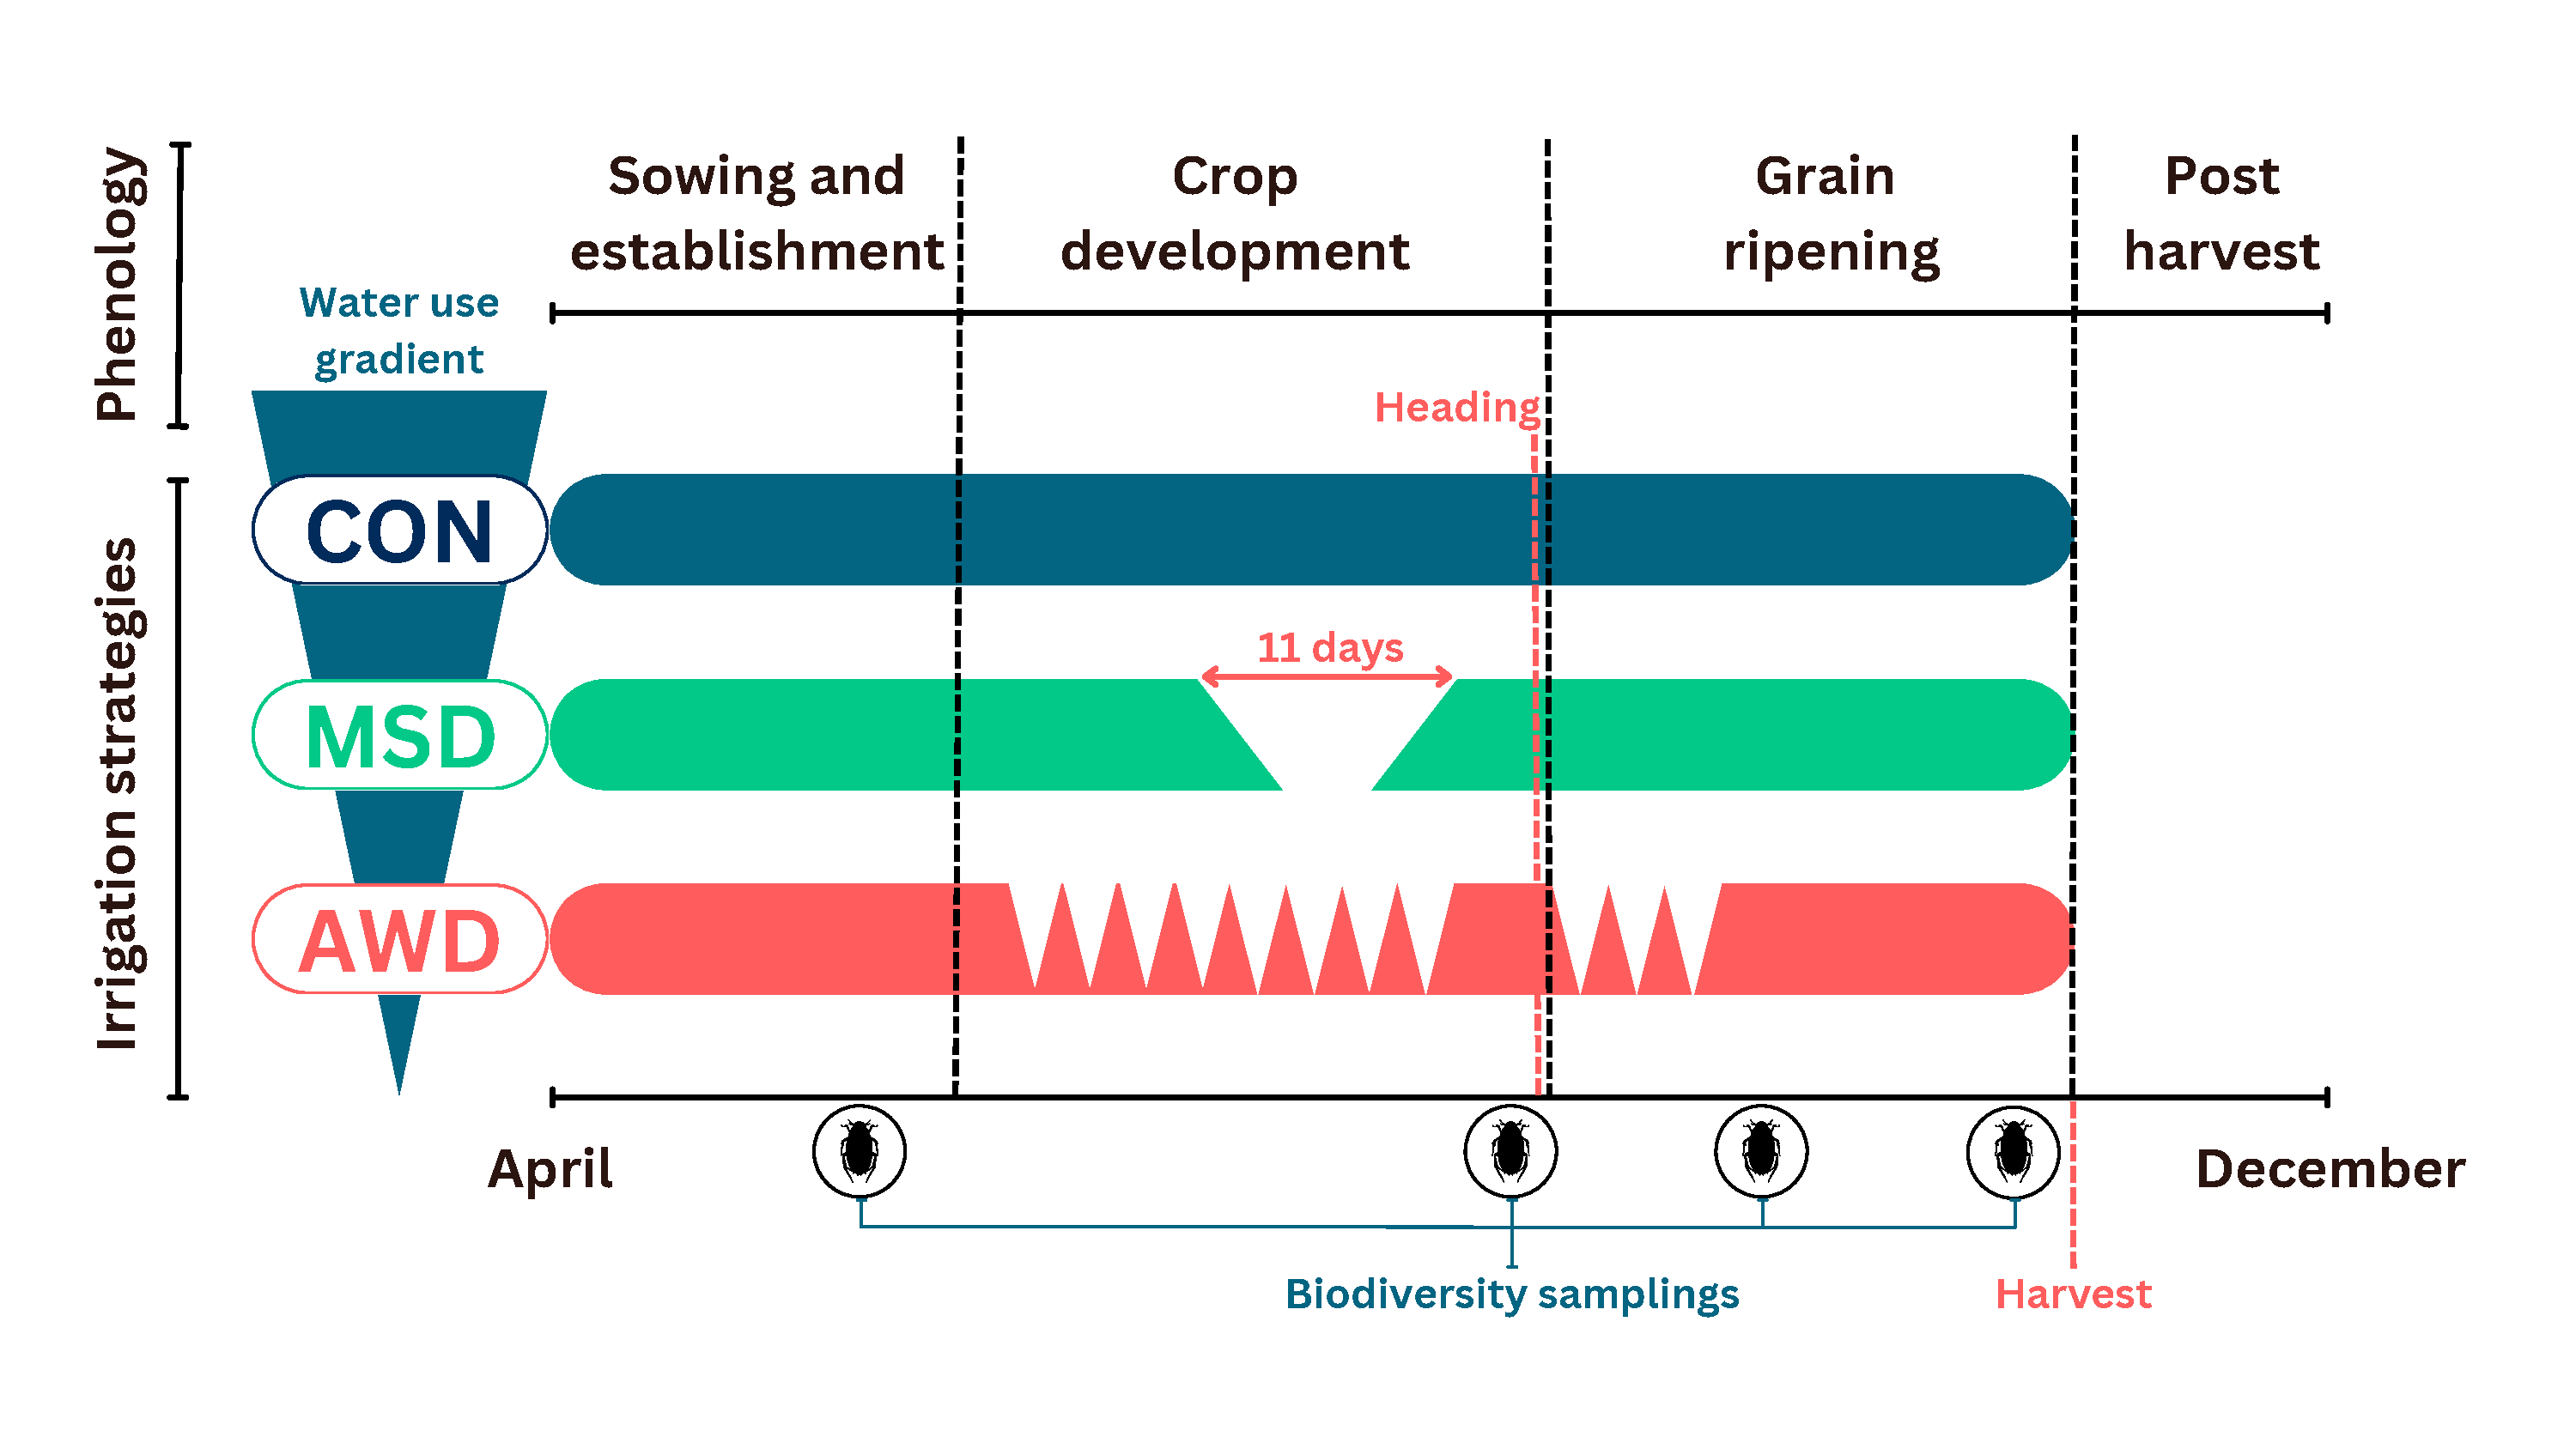
\includegraphics[scale=0.3, center]{Figures/Chapter_1/CERESTRES_Treatments.pdf}
	\captionof{figure}[Treats]{Water-saving irrigation strategies across the water use gradient. Horizontal bars represent reference water layer levels for each strategy through rice phenological stages. Biodiversity sampling dates are also represented across the season. Besides these, weekly greenhouse gas emissions and fortnightly aquatic vertebrate (fish and amphibians) and crayfish abundance samplings were carried out and are not represented in this figure. Abbreviations for assessed irrigation strategies stand for: CON = continuous flooding; MSD = mid-season drainage; and AWD = alternate wetting and drying.}   
	\label{Exp.des}
\end{figure}
%\vspace{0.5cm}\\

Three irrigation practices were tested in a complete randomized block design with five blocks. Each block consisted of three 10 $\times$ 11 m plots, each individually managed under one of the irrigation strategies (Figure \ref{Exp.lay}). Treatments corresponded to tested water-saving irrigation strategies (Figure \ref{Exp.des}): (i) conventional continuous flooding, where plots remained flooded from sowing (May) until two weeks before harvest (September); (ii) mid-season drainage (MSD), draining once, for a 11 days period (from June 30$^{th}$ to July 11$^{th}$, 2022), approximately 20 days before heading; and (iii) alternate wetting and drying (AWD), maintaining fields flooded until 4$^{th}$ leaf stage and from heading to the end of flowering, and under a flooding-drainage cycle through all other periods within the growing season (Table \ref{field_mgmt}). Such flooded periods within the AWD strategy are necessary to avoid physiological stress during emergence, early seedling  and flowering, which are the most sensitive drought-sensitive phenological stages \citep{singh2017developing, yang2019different}. Individual plot management was achieved thanks to independent water inflow and outflow at each plot (Figure \ref{Exp.lay}). Water level was controlled through the installment, and constant monitoring, of piezometers in MSD and AWD plots. AWD is the most widely adopted water-saving irrigation strategy, with reported improved water use efficiency of 18.0-63.0\%, depending on the saturated volumetric water threshold considered for re-flooding, usually termed as AWD severity \citep{linquist2015}. The technique has been improved to minimize yield impacts through the establishment of water table depth thresholds bellow soil surface (usually 15 cm) to trigger field flooding \citep{carrijo2017}, this practice is referred to as Safe-AWD or Mild-AWD. Besides intermittent flooding, MSD was evaluated as a second alternative practice with the objective of establishing a treatment intensity and water use gradient. Treatment intensity is defined by the frequency of dry periods through the growing season. This gradient presents its highest intensity with AWD management (low water use), medium intensity with MSD (medium water use) and lowest intensity with continuous flooding irrigation (high water use). All three treatments followed local conventional practices regarding fertilization, pest and disease control, and straw incorporation. All plots were seeded with JSendra, commercial round rice variety across Spain, and the most prevalent in the Ebro Delta.\\

\begin{table*} [htbp]
    \centering
    \footnotesize  
        \caption{Crop treatments and irrigation management schedule.}
    \begin{tabular}{l l}
\cline{1-2}
{Date} & {Management} \\
\cline{1-2}
%\rule{0pt}{3ex} % inserts space
{10-May-22} & {Fertilization (granulated controlled-release; NPK=33-9-6; 190 kg ha$^{-1}$)} \\
{13-May-22} & {Flooding (all plots)} \\
{17-May-22} & {Sowing (var. JSendra; 500 seeds m$^{-2}$)} \\
{31-May-22} & {Herbicide treatment (Clincher)} \\
{13-Jun-22} & {Start drain-flood cycles in  AWD plots} \\
{30-Jun-22} & {MSD plots drained} \\
{30-Jun-22} & {Herbicide treatment (Logan + Kaos)} \\
{11-Jul-22} & {MSD plots re-flooded} \\
{31-Jul-22} & {Fungicide treatment (Trifloxystrobin)} \\
{11-Aug-22} & {End of drain-flood cycles in  AWD plots} \\
{15-Sep-22} & {Final drain (all plots)} \\
{29-Sep-22} & {Harvest} \\
\cline{1-2}
    \end{tabular}
    \label{field_mgmt}
\end{table*} 


\subsection{Greenhouse gas flux measurement}
\label{sec:meth_GHG}

Gases were sampled through the non-steady state gas chambers method adapted from \cite{martinez-eixarch2018} on a weekly basis from mid-May to late-September 2022. Due to time restrains, samplings were done in three of the total five blocks (i.e., considering three plots per irrigation strategy). Chambers made of polyvinylchloride (PVC) squared frames and covered by transparent plastic were equipped with two ports, sealed with rubber septa, for the insertion of a thermometer and of sampling syringes. The chamber dimensions (129 cm$^{2}$ basal area and 72 cm height) allowed  their installation including several rice plants inside throughout the plant growth, as they were taller than plant height at harvest. Removable foam was set at the base of chambers to allow buoyancy through flooded periods, it was removed when fields were dry. This foam prevented gas exchange between the chamber headspace and the exterior, whereas wet towels were used with this purpose when foam was removed. Chambers were installed and removed for every sampling at the same location within plots. During gas samplings, four gas samples (30 ml) were extracted from each chamber every 10 minutes over a 30-minute period and then transferred over-pressured to pre-evacuated 12 ml vials. Samplings where done consistently from 10:00 to 15:00 to minimize variation derived from daily temperature variability. For every sampling date, soil (electrical conductivity, temperature, redox potential and pH, all measured at 10 cm-depth.) and water (temperature, salinity, oxygen concentration, oxygen saturation and pH) physicochemical parameters were assessed using an automated YSI Professional Plus (Pro Plus) Multiparameter Instrument (Brannum Lane, USA), a Hanna Instruments HI 98190 pH/ORP pH-meter and a Fieldscout direct soil E.C. meter (Spectrum Technologies, 2019). Rice cover (\%) was also recorded during each sampling. CH$_{4}$, CO$_{2}$ and N$_{2}$O concentrations were determined simultaneously using a GC 7820A Agilent (USA) system equipped with a single channel and 2 valves of ten-port gas sampling with back-flush to vent, and 6-port to change between the FID and micro-ECD detectors, using 2 packed columns Hayesep-Q 80-100 mesh 2 m x $1/8''$ x 2.0 mm Ultimetal Agilent (USA), according to \cite{arias2025determination}. The chromatograph calibration was done using CH$_{4}$ standards in nitrogen provided by Carburos Metalicos S.A. (Spain). Temperature variations within headspace of chambers were used to correct gas concentrations according to the ideal gas law. CH$_{4}$ emission rates were calculated as the slope of the linear regression between gas concentration and sampling time. Regressions were considered significant and their slopes accepted as emission rates if they were positive and \textit{R}$^2$ $>$ 0.70, whereas rates below this threshold were considered non-significant linear trends, due to being lower than the method's detection limit or products of ebullition induced by chamber installation, and were given the value of zero \citep{schultz2023}. Besides complete models considering all four measurements per sampling, four alternative models were also assessed, each removing one measurement step-wise and leaving only three remaining measurements. When model requirements were met by the alternative models but not by complete models, the alternative model with higher \textit{R}$^2$ was selected to calculate emissions (calculation example in Figure \ref{mod_exp}). This way, all calculated emission rates considered at least three measurements, the slopes corresponded to those of the best fitting linear models and any potentially altered measurements, due to possible chamber installation issues, were removed from calculations. Seasonal mean cumulative C-CH$_{4}$ emissions (kg ha$^{-1}$) were calculated for each individual plot considering constant rate in between samplings. \\

\subsection{Biodiversity assessment}
\label{sec:meth_BIO}

\replaced[id=SE]{Fish, amphibians and red swamp crayfish}{Aquatic vertebrate (\textit{Carassius carassius}, \textit{Pseudorasbora parva} and \textit{Misgurnus anguillicaudatus} fish species, and \textit{Pelophylax perezi} tadpoles) and red swamp crayfish (\textit{Procambarus clarkii})} communities \added[id=SE]{(Table \ref{AbuMacroFauna})} were characterized sampling individuals fortnightly through the rice growing season installing two cylindrical static nets per flooded plot, identifying to the species level and counting trapped individuals after 24 hours. \added[id=SE]{These samplings were implemented with the objective of capturing the effects irrigation strategies might have on abundance throughout the season, and were later used to compare the resulting cumulative abundance in between strategies across the complete assessed period. }Benthic macroinvertebrate (i.e., different insect groups and juvenile red swamp crayfish) sample collection was carried out separately to fish, amphibians and adult red swamp crayfish using a dip net (250 $\mu$m). Sampled water volume was kept homogeneous by making four net collections across a 30 $\times$ 30 cm plastic frame for each sub-sample. The net was submerged at 1 cm below soil level to collect individuals from the water layer as well as those living just above the soil-water interface. This process was repeated four times per plot and then all collected sub-samples were combined in one recipient, resulting in one final sample per plot. Samples were then washed and stored in 70$\%$ ethyl alcohol for later processing. Macroinvertebrate sample collection was repeated four times through the growing season (June 10$^{th}$, July 15$^{th}$ and August 2$^{nd}$ and 31$^{st}$, 2022) to assess potential changes in community structure and dynamics associated to the irrigation strategies. Sample processing consisted in washing each recipient's content through a 500 $\mu$m mesh sieve and individualizing aquatic organisms (i.e., excluding plant material and terrestrial macroinvertebrates that might have fallen into the traps). Collected organisms were then identified up until the highest possible taxonomic resolution by an experienced taxonomist. Individuals that could only be identified up to a certain level (i.e., order, family or genus), were afterwards assigned to higher levels according to the weighted proportion of individuals in these higher levels.

\subsection{Crop yield}
\label{sec:meth_Yield}

All experimental plots were drained before harvesting to allow machinery entrance. Mechanical harvest was carried out and final yield (kg ha$^{-1}$) was registered per plot to assess potential impacts of water-saving irrigation strategies over production. Yield was calculated as wet weight, immediately after the harvest.  

\subsection{Data analysis}
\label{sec:meth_Stat}

The effect of water-saving strategies on CH$_{4}$ emission rates was analyzed through the application of a generalized linear mixed-modelling (GLMM) approach (model structures are summarized in Table \ref{mod_str}). The CH$_{4}$ emission rate was defined as the dependent variable within models, while the interactions between water-saving strategies and sampling dates were considered as fixed effects (\textit{n} = 213 observations). This interaction was assessed to account for potential temporal variation in the effects of these water regimes on CH$_{4}$ emissions. Soil and water physicochemical parameters were included as covariates within the model after correlation (through Spearman's rank, Figure \ref{Corr_plot}, and Pearson correlation coefficient, Figure \ref{Dendro}) and collinearity (through variance inflation factor, VIF) assessments. Covariates with Pearson's correlation coefficient over 0.75 or VIF over 5 were not included in models. Random effects were accounted for in the model using repetitions (i.e., five replicated blocks) as grouping factor. Gaussian distribution and \textit{identity} link function were applied in the model.\\

The impact of water-saving irrigation strategies on macroinvertebrate communities was evaluated from the perspectives of abundance and diversity. Accumulated abundance (number of total sampled individuals) through the entire rice growing season was assessed for all experimental plots using a subset of the complete biodiversity sampling results. In this, only larvae from water beetles (Coleoptera), water bugs (Hemiptera), dragonflies and damselflies (Odonata) were considered. These three groups were selected in order to work with a single functional group, as they represent the majority of top aquatic predators \citep{lawler2001}. Furthermore, they presented the highest number of species and could be identified to higher taxonomic levels. All individuals in adult stadiums were excluded to avoid potential mobility in between plots, thus focusing the analysis on less mobile individuals more representative of effects on biodiversity due to their higher susceptibility to drainage. Besides these three macroinvertebrate groups, abundance analysis was extended considering decapoda (red swamp crayfish), fish and amphibians (\textit{Pelophylax perezi} tadpoles). Individuals were grouped among orders as maximum taxonomic level to simplify analysis. This first analysis complements posterior diversity analyses, allowing the assessment of any potential effect of irrigation treatments on the amount of individuals per taxonomic level, independent of communities' diversity.  Effects on accumulated abundance of individuals were assessed through a GLM considering abundance as dependent variable and the interaction between irrigation strategy and taxonomic identity as fixed effects (Table \ref{mod_str}). No additional covariates were considered.\\ 

Effects on the diversity of these communities were analyzed considering only macroinvertebrates from the same taxonomic subset as for the abundance analysis. Decapoda, fish and amphibians were excluded due to being composed only by one (i.e., decapoda and amphibians) or very few species (i.e., fish) and, therefore, not representing potential diversity variations. Species richness (\textit{q$_{0}$}) and Shannon diversity (the exponential of  Shannon index, or \textit{q$_{1}$}) for each experimental plot were estimated using the iNext R package (Hill numbers; \cite{chao2014a, hsieh2016}). Both estimations characterize biodiversity profiles within rice fields, species richness indicates the total number of observed species and Shannon diversity can be interpreted as the effective number of common or typical species in the community \citep{chao2014}. Data analysis was done using GLMMs considering biodiversity indexes (\textit{q$_{0}$} and \textit{q$_{1}$}) as each model's dependent variable, the interaction between irrigation strategies and the square of sampling dates as fixed effects, and blocks to account for random effects. A quadratic relation was identified between both biodiversity indexes and sampling date, therefore, the square of sampling (sampling 1 to 4) was included in the model. Soil and water physicochemical parameters were included as covariates after checking for correlation and collinearity, under the same criteria as for CH$_{4}$ emission analysis. For Shannon diversity, a strong interaction was observed between conductivity and water strategies (Figure \ref{vars_Treat}), so it was removed from the model as an explanatory variable to avoid artifacts and isolate the treatments' effect. All abundance and biodiversity models used Gaussian distribution and \textit{identity} link function. Crop yield variations among the assessed strategies were analyzed fitting a linear model considering yield and irrigation treatment as dependent and independent variables, respectively.\\

Data management, visualization and analysis was carried out using R software (R-4.2.2). GLMMs were fit using the \textit{glmmTMB} package \citep{brooks2017}. All models were analyzed through residual diagnostics and R$^{2}$, collinearity and singularity analyses using the \textit{DHARMa} \citep{hartig2018dharma} and \textit{performance} \citep{ludecke2021} R packages, respectively. Analyses of variance (ANOVA) were carried out for all models to identify significant effects. For all cases where different effects were contrasted for factor levels, the \textit{emmeans} package was used \citep{lenth2017}.  

\section{Results}
\label{sec:results}

\subsection{Climate change mitigation} 

Irrigation strategies had a significant effect on C-CH$_{4}$ emission rates ($\chi^2$=59.3, \textit{p}=$<$0.001; Figure \ref{CH4_acc}; results for all ANOVA tests are summarized in Table \ref{mod_res}). Lower rates were identified for both non-continuous irrigation treatments, MSD (\textit{t}=-6.7, \textit{p}=$<$0.001, results for all estimated marginal means paired comparisons are summarized in Table \ref{mod_pairs}) and AWD (\textit{t}=-6.5, \textit{p}=$<$0.001), when compared to conventionally flooded plots. There is high variation among rates from different irrigation managements across the season, evidenced by the significant interaction between irrigation strategies and sampling dates ($\chi^2$=64.8, \textit{p}=$<$0.001). No soil or water physicochemical parameter showed significant effects on emission rates. Considering the overall seasonal emission rate mean, MSD and AWD strategies achieved 69.0\% and 94.0\% decrease in CH$_{4}$ emission rates, respectively, when compared to continuous flooding strategy (continuous flooding = 2.2 $\pm$ 0.3 mg m$^{-2}$ h$^{-1}$; MSD = 0.7 $\pm$ 0.1 mg m$^{-2}$ h$^{-1}$; AWD = 0.1 $\pm$ 0.003 mg m$^{-2}$ h$^{-1}$). Mean cumulative C-CH$_{4}$ emissions for the whole growing season were 64.2 kg ha$^{-1}$, 21.0 kg ha$^{-1}$ and 4.8 kg ha$^{-1}$ for plots managed under continuous flooding, MSD and AWD strategies, respectively. Emissions from non-continuous flooding plots were reduced in 67.3\% with MSD strategy and in 92.5\% with AWD management, when comparing to continuous flooding plots.\\ 

\begin{figure} [ht]
\captionsetup{justification=justified}
	\centering 
	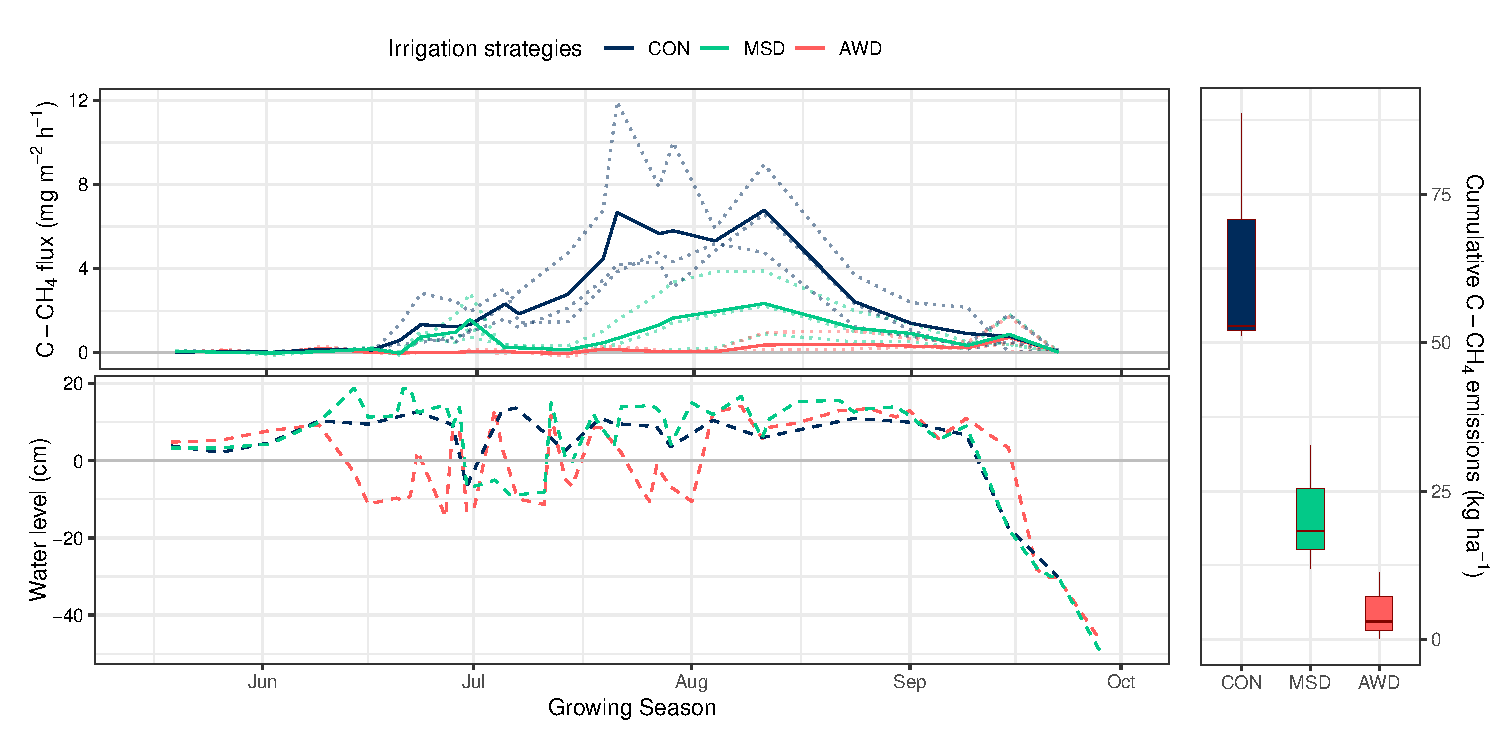
\includegraphics[scale=0.65, center]{Figures/Chapter_1/CH4_flux_water_acc.pdf}
	\captionof{figure}[CH4]{Methane (C-CH$_{4}$) emission rates (top-left panel, in mg m$^{-2}$ h$^{-1}$) and water level (bottom-left panel, in cm) across the rice growing season for the three water-saving irrigation strategies. Discontinuous lines in the top-left panel are mean emissions per plot, continuous lines are treatment means. Right panel shows cumulative C-CH$_{4}$ emissions in kg ha$^{-1}$ for the  rice growing season. Abbreviations for assessed irrigation strategies stand for: CON = continuous flooding; MSD = mid-season drainage; and AWD = alternate wetting and drying.}  
	\label{CH4_acc}
\end{figure}
%\vspace{0.5cm}

\subsection{Biodiversity conservation} 

 Significant differences were identified among irrigation strategies regarding accumulated abundance of vertebrate and macroinvertebrate individuals across the growing season ($\chi^2$=53.2, \textit{p}=$<$0.001), yet a significant statistical interaction between irrigation strategies and taxonomic groups was observed ($\chi^2$=46.2, \textit{p}=$<$0.001). An overall decrease in abundance was observed for AWD plots when compared to continuously flooded plots for most of the assessed taxonomic groups, except for coleoptera and fish (Figures \ref{Abu} and \ref{Abu_date}; and Tables \ref{AbuColOdoHet} and \ref{AbuMacroFauna}). The most extreme effect was observed for amphibians, where abundance tended towards zero values within AWD plots, hindering variance analysis among the three strategies. When re-modelling for a data subset consisting only of amphibian individuals and excluding AWD plots, no difference was identified between MSD and continuous flooding ($\chi^2$=0.3, \textit{p}=0.586). For most groups of aquatic organisms, intermediate abundance levels were achieved by MSD managed plots when compared to continuous flooding and AWD strategies (Figure \ref{Abu}).\\

\begin{figure} [ht]
\captionsetup{justification=justified}
	\centering 
	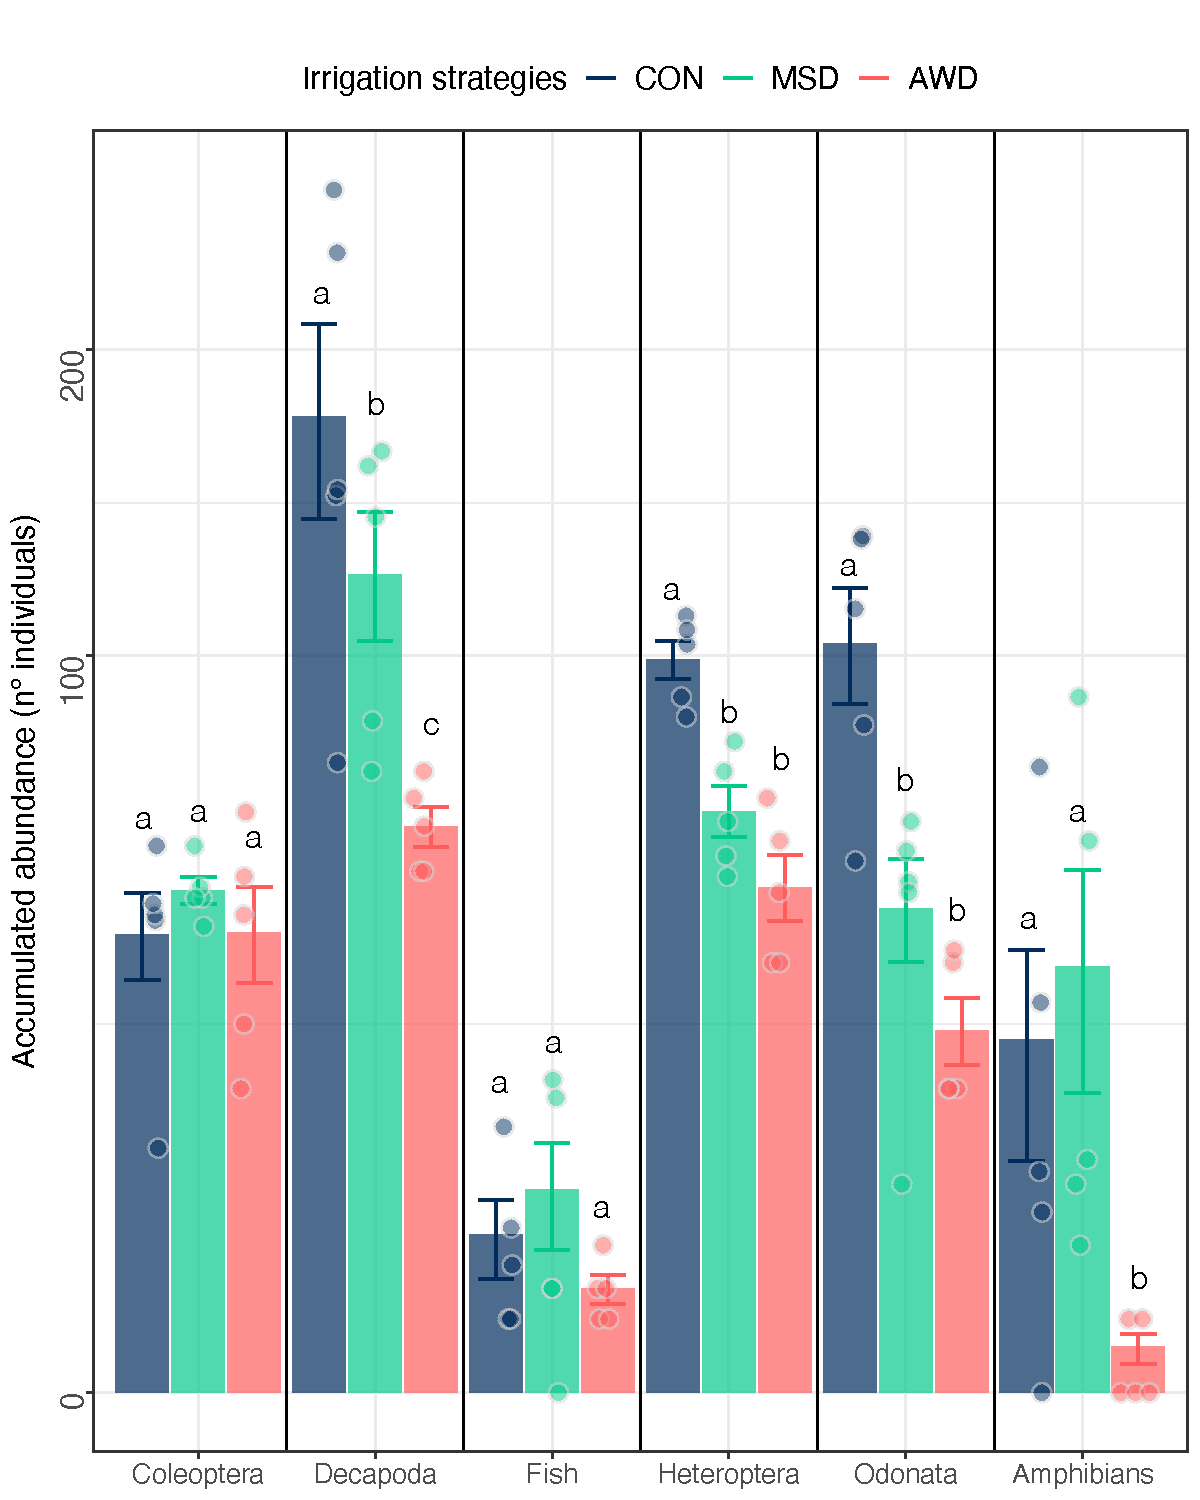
\includegraphics[scale=0.4, center]{Figures/Chapter_1/Abu.div_2022_avg_plots.9.pdf}
	\captionof{figure}[Abundance]{Accumulated abundance (number of individuals) of sampled macroinvertebrates, amphibians and fish for the three water-saving strategies across the rice growing season. Each bar shows the averaged abundance for all samplings and plots according to each strategy, points are abundance results per plot for each sampling and error bars indicate standard errors. Letters above bars show significant statistical differences among irrigation strategies. Abbreviations for assessed irrigation strategies stand for: CON = continuous flooding; MSD = mid-season drainage; and AWD = alternate wetting and drying.}   
	\label{Abu}
\end{figure}
%\vspace{0.5cm}

 Irrigation strategies did not have an overall effect on species richness of aquatic macroinvertebrates ($\chi^2$=3.6, \textit{p}=0.167; Figure \ref{Div_q0}a), but significant effects were observed for the interaction between strategies and the squared sampling dates ($\chi^2$=6.3, \textit{p}=0.043). Covariates with significant effect were the squared sampling dates ($\chi^2$=10.0, \textit{p}=0.002), sampling dates ($\chi^2$=6.6, \textit{p}=0.010), soil electrical conductivity (EC, in $\mu$S $cm^{-1}$; $\chi^2$=6.5, \textit{p}=0.010) and oxygen concentration in the water layer ($O_{2}\%$; $\chi^2$=5.4, \textit{p}=0.020). To further analyze the effect of sampling dates, the effect of irrigation strategies was studied for each independent sampling date, fitting individual GLMMs per each sampling date. A significant effect of irrigation strategy over species richness was identified for the second sampling date ($\chi^2$=71.6, \textit{p}=$<$0.001), but no such effect was evident for all other sampling dates (Figure \ref{Div_q0}b). Within this second sampling, both MSD (\textit{t}=7.1, \textit{p}=$<$0.001) and AWD (\textit{t}=7.8, \textit{p}=$<$0.001) strategies decreased species richness significantly compared to continuous flooding. During this second sampling, MSD and AWD strategies reduced average species richness by 53.0\% and 55.0\%, respectively, versus conventional flooding (continuous flooding = 9.8 $\pm$ 0.7; MSD = 4.6 $\pm$ 0.8; AWD = 4.4 $\pm$ 0.05). Soil pH showed a significant effect ($\chi^2$=11.1, \textit{p}=$<$0.001) on species richness for sampling 2.\\
 
 \begin{figure} [ht]
\captionsetup{justification=justified}
	\centering 
	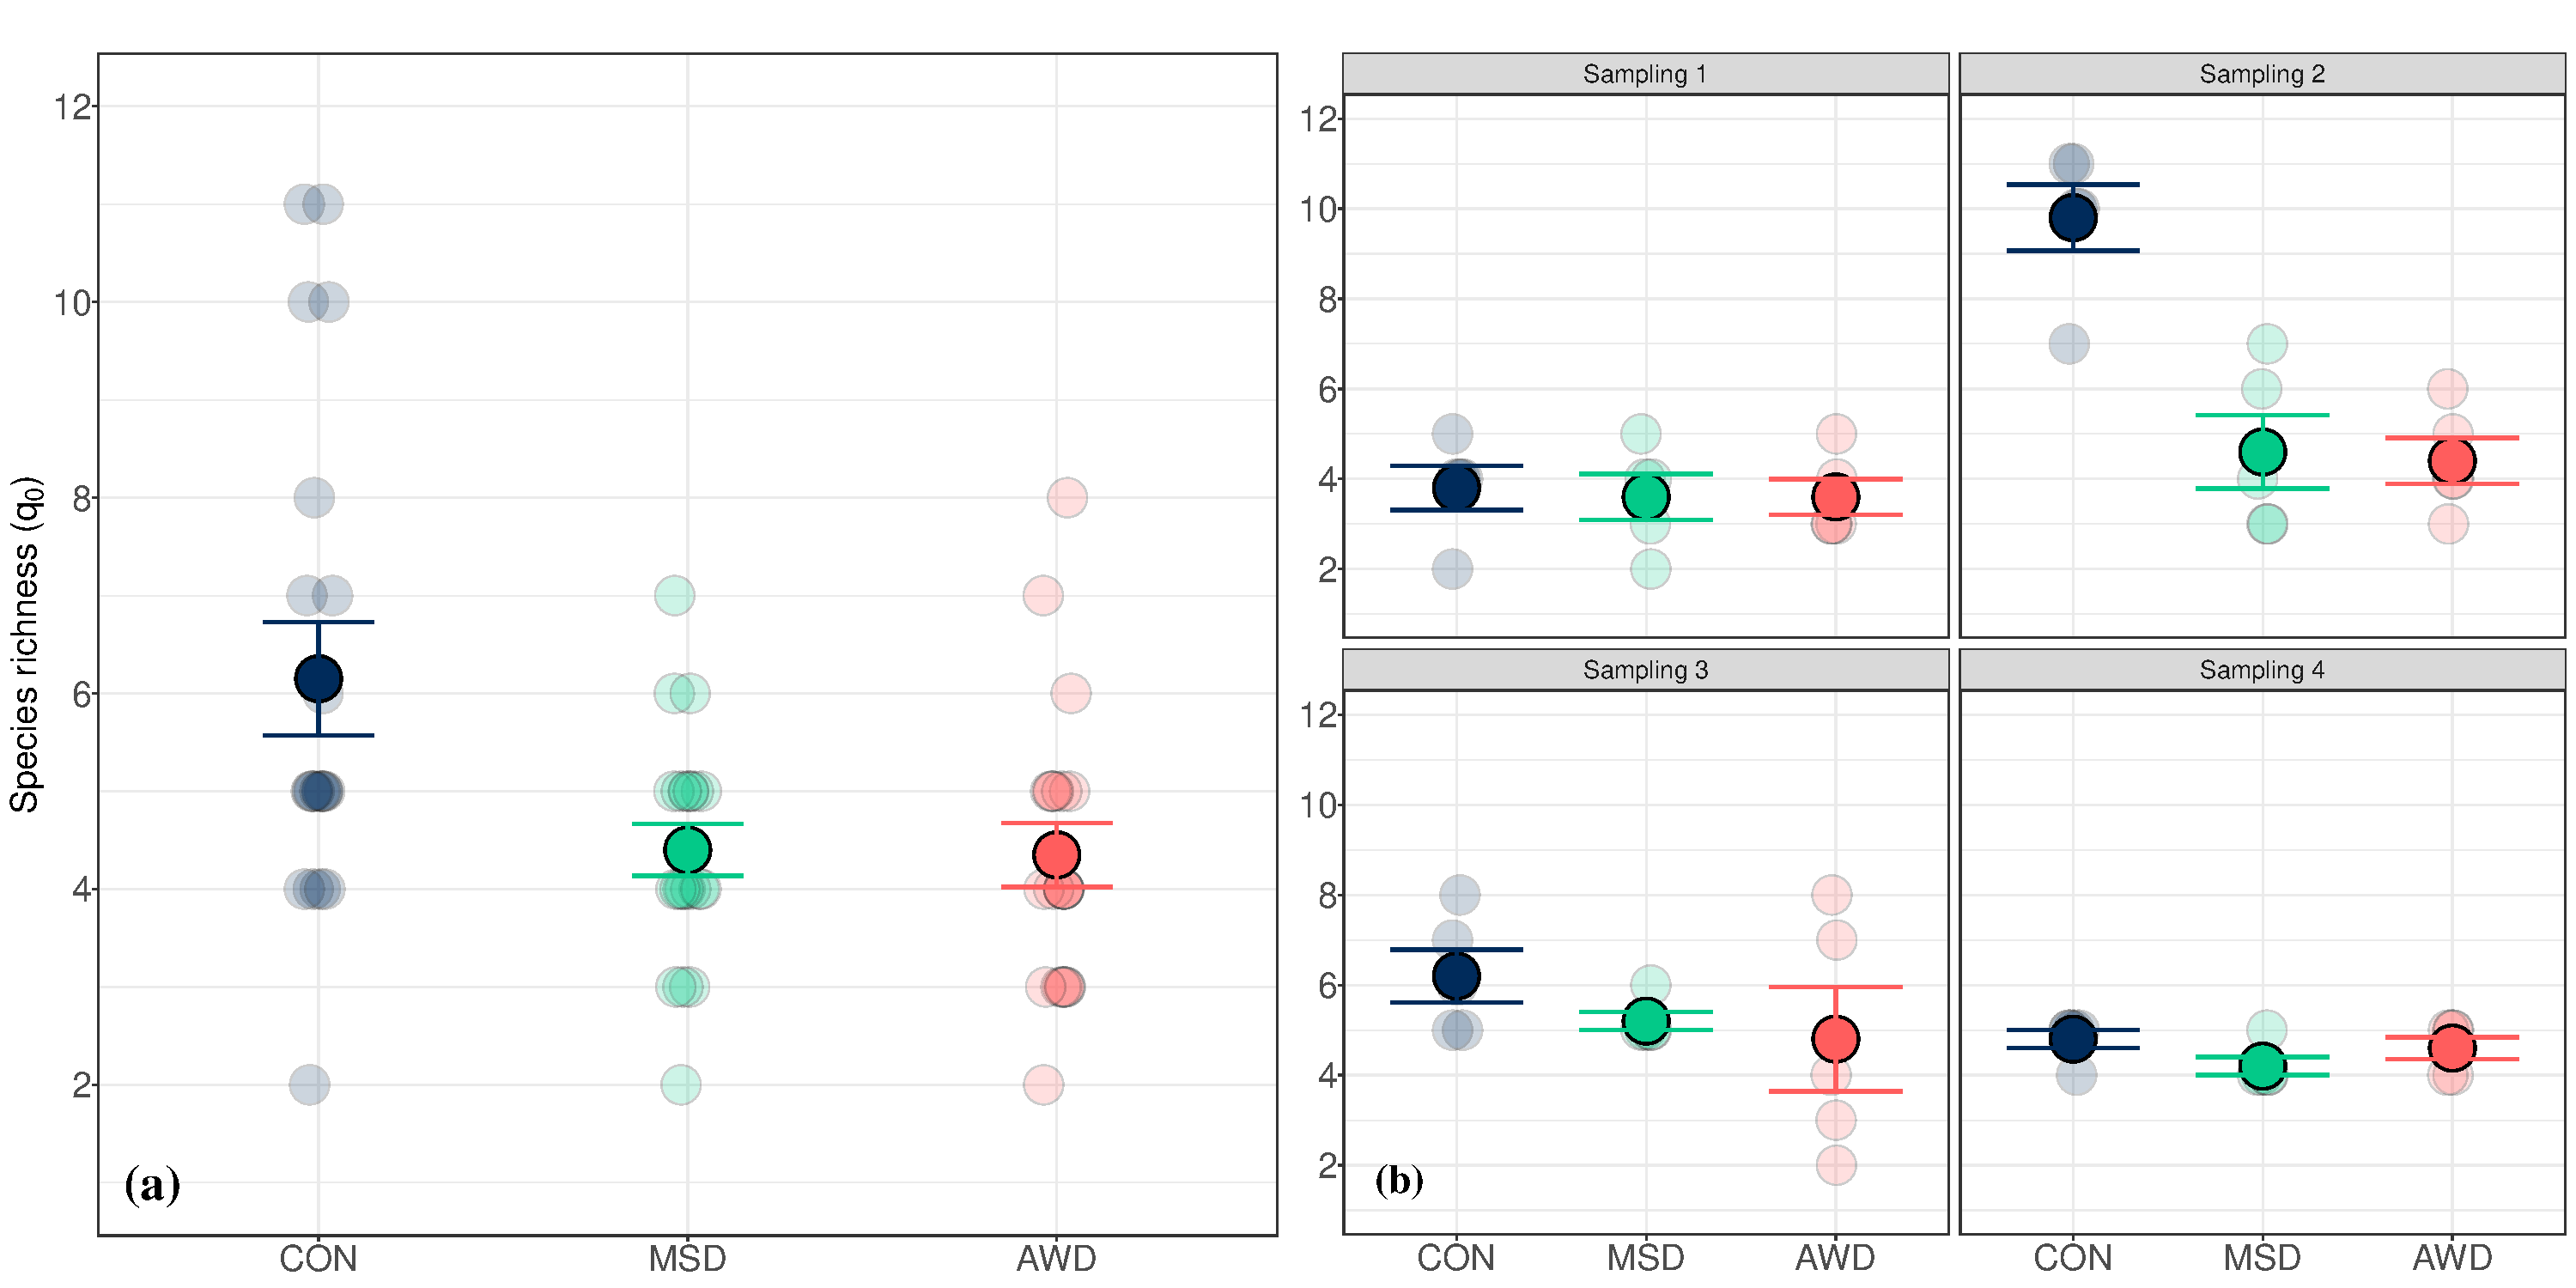
\includegraphics[scale=0.33, center]{Figures/Chapter_1/Arr.q0_ind.samp.pdf}
	\captionof{figure}[Species richness]{Macroinvertebrate species richness (number of identified species) for the three water-saving strategies. Semi-transparent points indicate plot means for each sampling date. Solid points and error bars indicate the overall means and standard errors, respectively. The left-hand panel \textbf{(a)} shows overall averaged results considering all four sampling dates across the rice growing season. The right-hand panels \textbf{(b)} show results for each sampling date separately. Abbreviations for assessed irrigation strategies stand for: CON = continuous flooding; MSD = mid-season drainage; and AWD = alternate wetting and drying.}   
	\label{Div_q0}
\end{figure}
%\vspace{0.5cm}

Shannon diversity varied significantly among different irrigation strategies ($\chi^2$=13.3, \textit{p}=0.001; Figure \ref{Div_q1}). Nevertheless, no significant effect was detected for AWD plots when comparing to continuous flooding strategy (\textit{t}=0.2, \textit{p}=0.973), while MSD resulted in lower diversity than both continuous flooding (\textit{t}=2.9, \textit{p}=0.017) and AWD (\textit{t}=-2.5, \textit{p}=0.040), contrary to the expected balancing effect. Significant effects were identified for sampling date ($\chi^2$=17.6, \textit{p}=$<$0.001), squared sampling date ($\chi^2$=17.4, \textit{p}=$<$0.001), soil pH ($\chi^2$=5.5, \textit{p}=0.018) and oxygen concentration ($\chi^2$=3.9, \textit{p}=0.047).

 \begin{figure} [ht]
\captionsetup{justification=justified}
	\centering 
	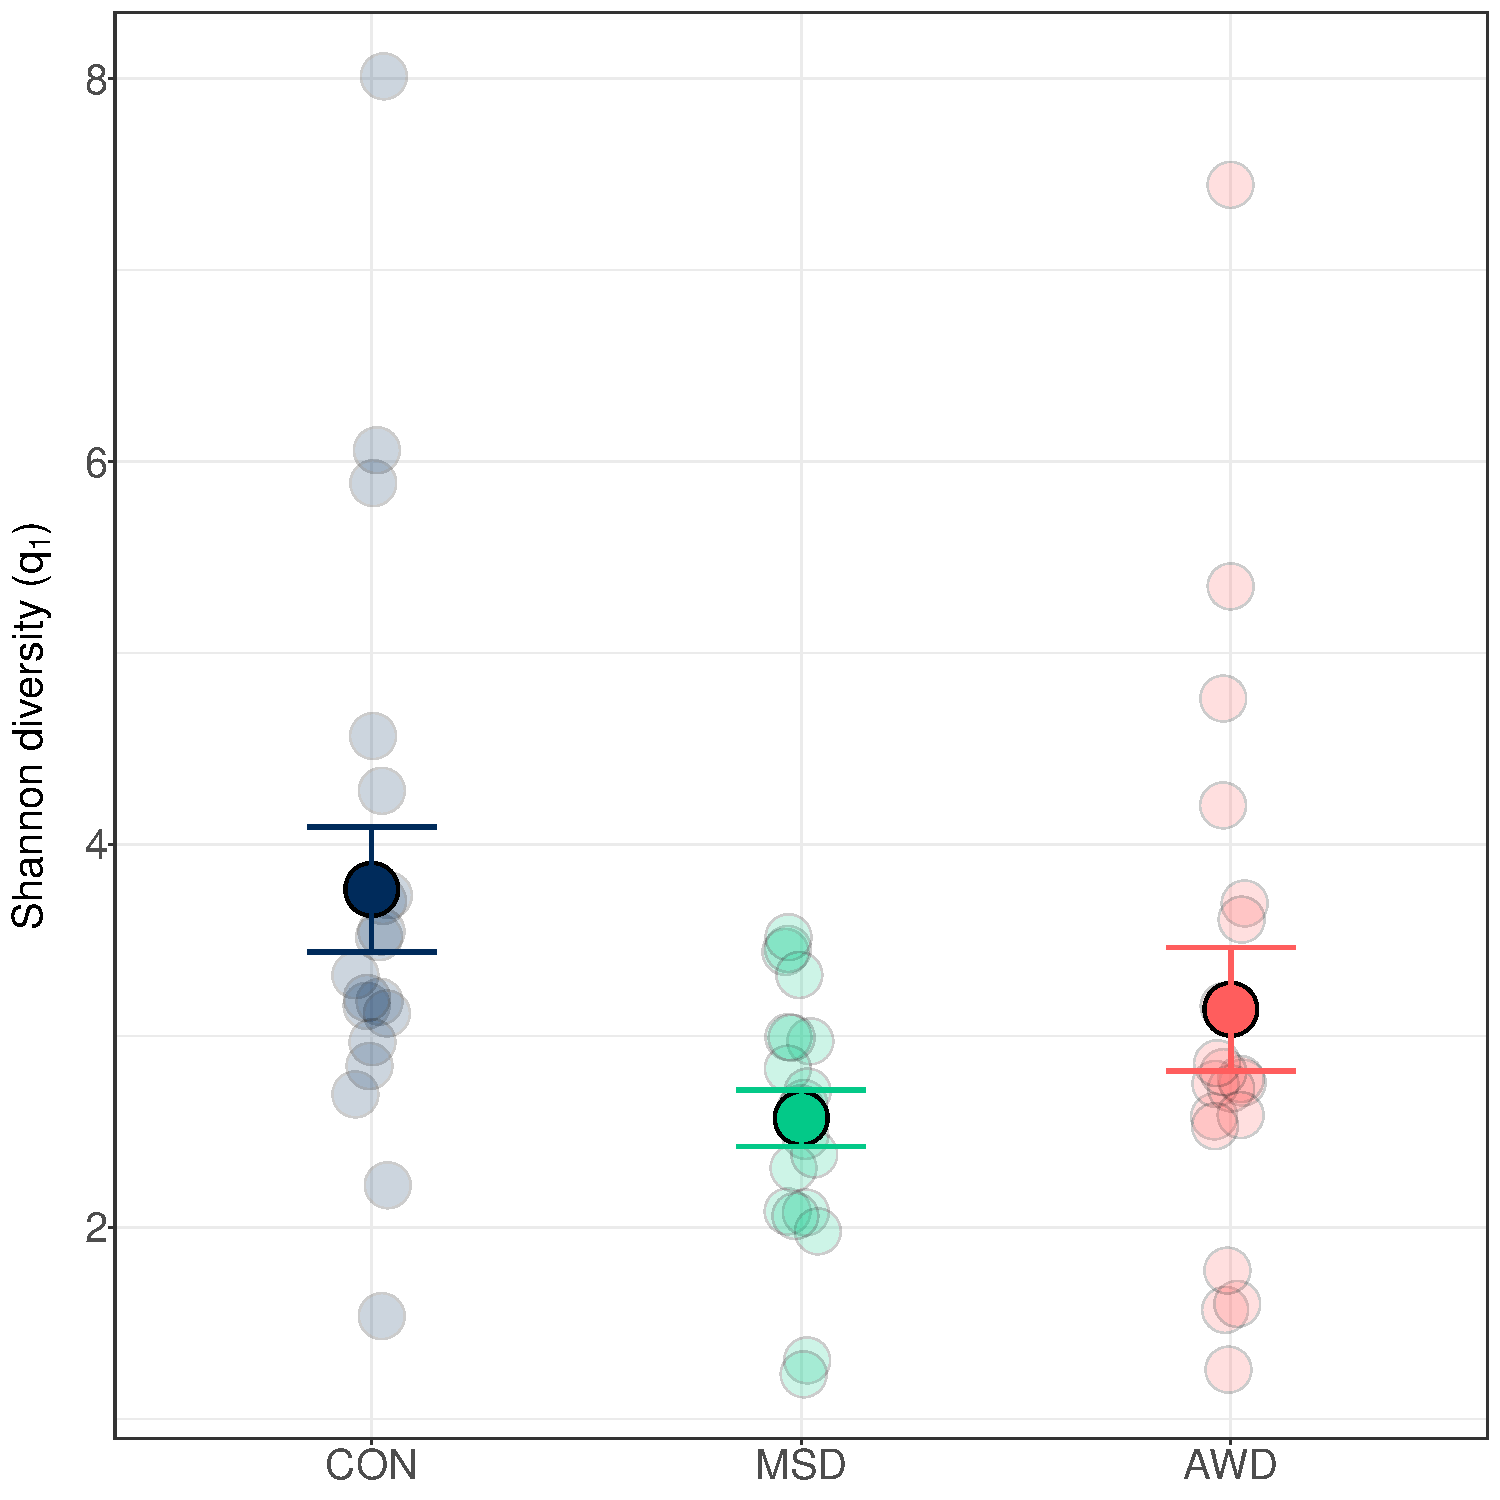
\includegraphics[scale=0.33, center]{Figures/Chapter_1/Shannon_indiv2.pdf}
	\captionof{figure}[Shannon diversity]{Macroinvertebrate Shannon diversity patterns for the three water-saving strategies. Semi-transparent points indicate plot means for each sampling date. Solid points and error bars indicate the overall means and standard errors, respectively. Abbreviations for assessed irrigation strategies stand for: CON = continuous flooding; MSD = mid-season drainage; and AWD = alternate wetting and drying.}   
	\label{Div_q1}
\end{figure}
%\vspace{0.5cm}

\subsection{Crop yield} 

Crop yields were influenced by water strategies (F=13.8, \textit{p}=$<$0.001). Implementing AWD as a high intensity and low water-use strategy, proved to reduce significantly final rice grain yield in comparison to both continuous flooding (\textit{t}=-4.4, \textit{p}=0.002, Figure \ref{Yields}) and MSD (\textit{t}=--4.7, \textit{p}=0.002) strategies. The mid-intensity MSD strategy, on the other hand, did not result in crop production declines against a continuous flooding strategy (\textit{t}=0.2, \textit{p}=0.968). Final mean yields were 8,213 ($\pm$176), 8,271 ($\pm$180) and 7,154 ($\pm$150) kg ha$^{-1}$, for plots under continuous flooding, MSD and AWD irrigation, respectively. A mean yield decrease of 12.9\% was observed for AWD when comparing to continuously flooded plots.

\begin{figure} [ht]
\captionsetup{justification=justified}
	\centering 
	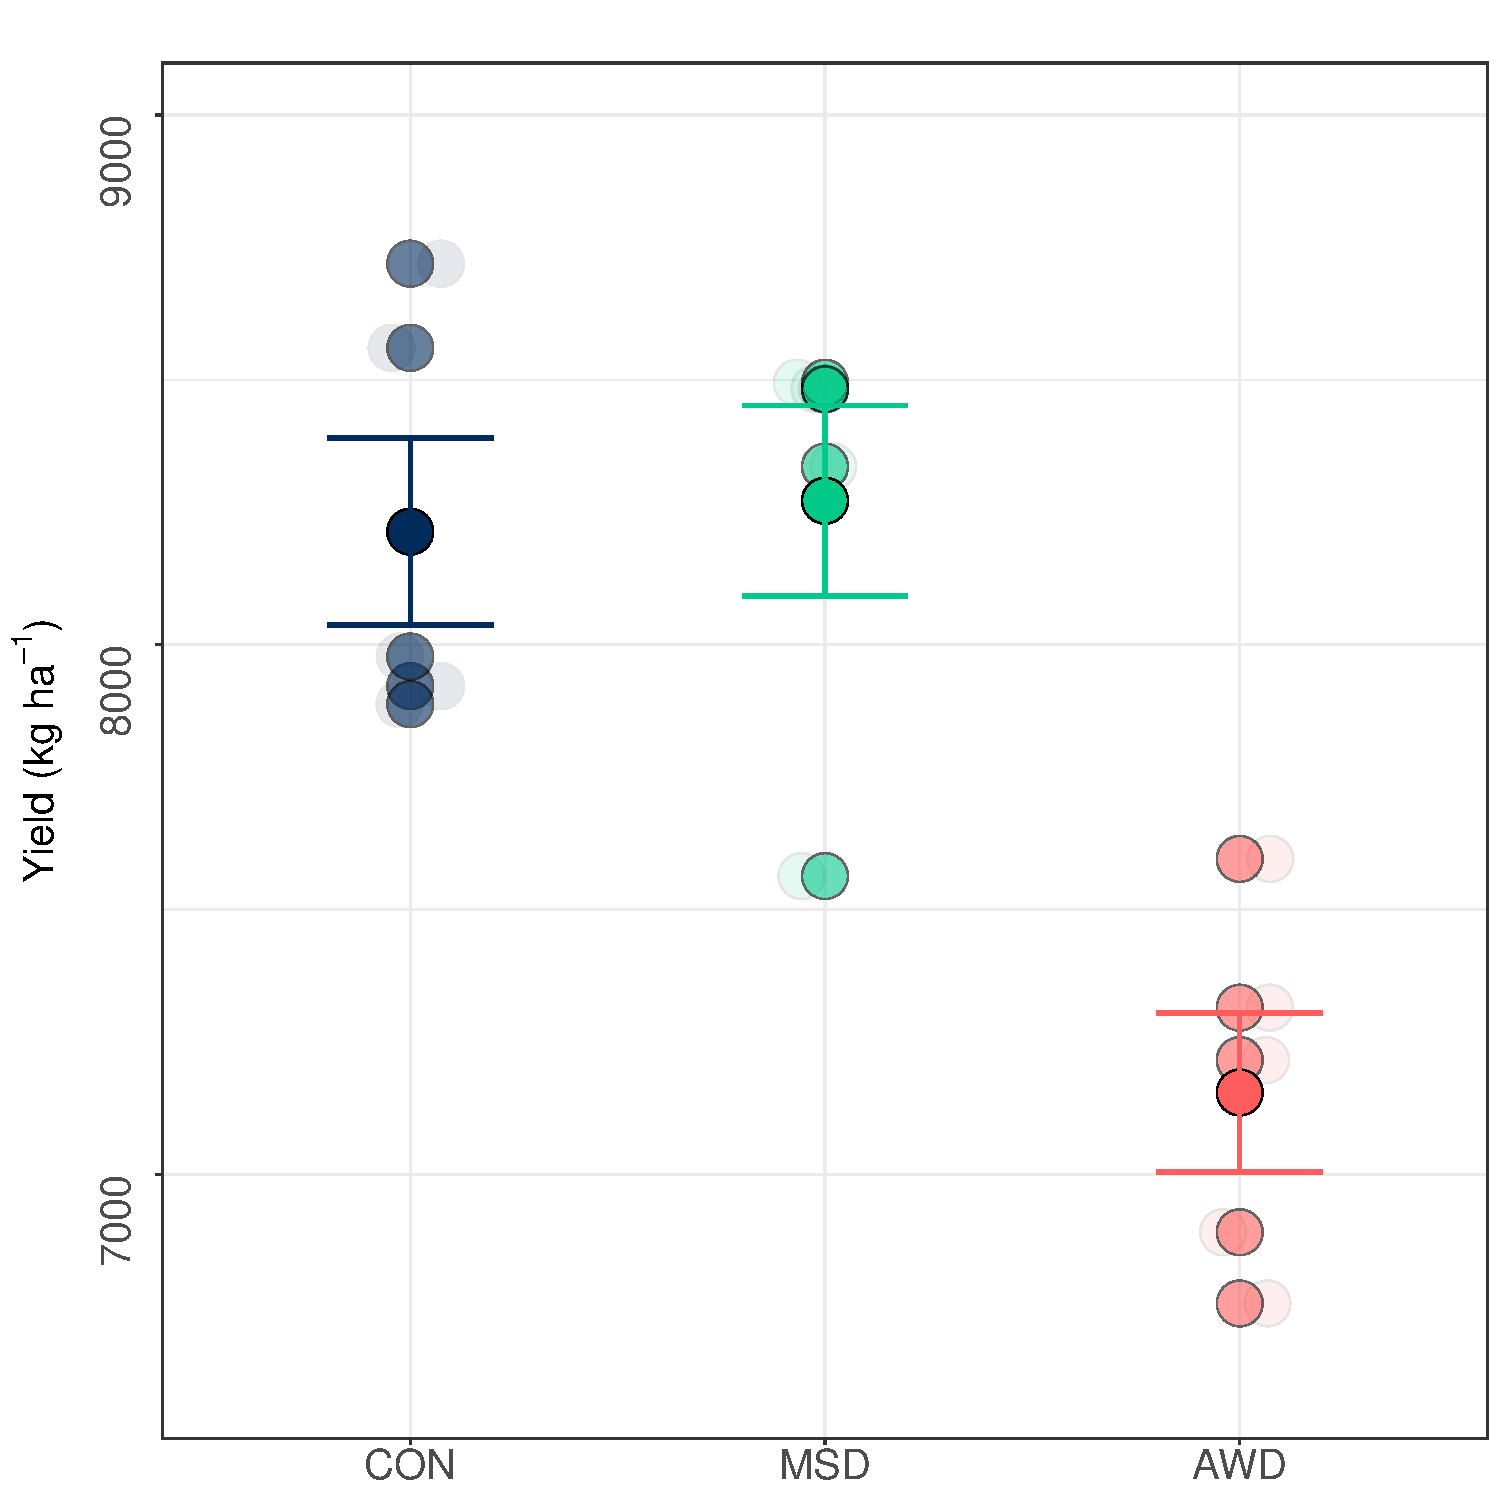
\includegraphics[scale=0.33, center]{Figures/Chapter_1/Prod_2022_plot2.pdf}
	\captionof{figure}[Yields]{Rice yields (kg h$^{-1}$) for all three water-saving strategies. Each bar shows the averaged yield for all plots according to each strategy, error bars indicate standard errors. Abbreviations for assessed irrigation strategies stand for: CON = continuous flooding; MSD = mid-season drainage; and AWD = alternate wetting and drying.}   
	\label{Yields}
\end{figure}
%\vspace{0.5cm}\\

\section{Discussion}
\label{sec:discussion}

Plenty of research effort has been focused on the development of water-saving irrigation strategies in rice paddy fields to adapt to more frequent severe droughts \citep{bouman2007, luo2019, shankar2021} and to mitigate climate change through a decline in CH$_{4}$ emission rates \citep{linquist2018}. Potential negative effects on biodiversity conservation of those species depending on rice water layers has, nevertheless, largely been overlooked. Through this study, the scope of agricultural management assessment is extended to include possible effects on these freshwater communities. \\

Regarding climate change mitigation, the assessed non-continuous flooding irrigation strategies resulted in positive effects, reducing CH$_{4}$ rates, as observed by several studies \citep{cai2003, li2006, lahue2016, lagomarsino2016, meijide2017}. Emission rates from AWD managed plots remained close to zero all across the flooding-drying cycle, pattern that has already been observed \citep{balaine2019}. This effect is attributed to aerobic oxidation by methanotrophs and reduced methanogenic activity \citep{kumar2019alternate}. Although a meta-analysis by \cite{jiang2019} found that non-continuous flooding practices reduced CH$_{4}$ emissions in average by 53\% compared to continuous flooding, these impacts are variable throughout the literature and high reductions as those observed in the present study (92.5\%) are in line with previous observations in temperate rice production regions. In Italy, \cite{peyron2016} eliminated completely CH$_{4}$ emissions through AWD, maintaining oxic conditions through most of the growing season. In California, AWD has been reported to decrease CH$_{4}$ emissions up to 87\% \citep{lahue2016} and 93\% \citep{linquist2015} in relation to continuous flooding, attributing such large effects to soils drying more in between flood events than in studies where no such large decreases were observed, and to drainage timing. Maximum emission decreases are achieved if drainage is implemented when \citep{fertitta-roberts2019}, or a few days before \citep{souza2021}, emission peaks are observed in continuously flooded fields. In regions in which CH$_{4}$ emissions peak early in the season (e.g. China), but keep fields flooded or drain them late in the growing season, there is a large mitigation potential to reduce CH$_{4}$ emissions \citep{qian2023}. Emissions from MSD plots increased similarly to those conventionally managed during the beginning of the season (mid- to late-June, Figure \ref{CH4_acc}), but collapsed to levels closer to AWD plots as soon as the drainage period was implemented. Right after these plots were re-flooded, emissions recovered steadily but did not return to continuous flooding levels. This two-peaked pattern in CH$_{4}$ emission fluxes has been observed frequently for MSD water management in rice paddy fields \citep{sass1992, yagi1997}. Emission rates and seasonal accumulated CH$_{4}$ emissions respond to the water-use gradient, with highest emissions in conventional plots and lowest in AWD plots \citep{islam2022, perry2022}. The MSD irrigation served, as expected, as a balancing strategy in between both gradient extremes. Results are in good agreement with those found in previous studies, which report reductions of up to 95.0\% for AWD \citep{martinez-eixarch2021} and 66.0\% for MSD \citep{balaine2019} in seasonal cumulative emissions, when compared to continuous flooding strategies.\\

The impact of water saving techniques on freshwater biodiversity in rice plots are evident when comparing abundance of aquatic organisms among differently irrigated plots. There is a marked negative effect on vertebrate and macroinvertebrate abundance when comparing AWD with both continuous flooding and MSD strategies. For most of the assessed groups of organisms, there is a decreasing trend in overall abundance, with more individuals sampled in continuously flooded plots, followed by MSD and, finally, AWD. Multiple short hydroperiods associated to AWD rice fields might avoid the completion of active aquatic phases for many invertebrates and amphibians \citep{lawler2001}. The strong abundance decline in aquatic macroinvertebrates present in AWD plots might be attributed to the fact that univoltine (one brood per season) predator insects are susceptible to drainage in intermittently irrigated rice fields, which might prove positive for multivoltine prey species, like mosquitoes \citep{mogi1993}. The impact of short hydroperiods is especially evident for amphibians, for which the absence of tadpoles in AWD managed plots indicated a collapse in \textit{Pelophylax perezi} recruitment. AWD managed plots act, therefore, as ecological traps for amphibians, which is the group of vertebrates most threatened by habitat transformation \citep{amphibians}. \cite{watanabe2013} reported negative effects of MSD irrigation on abundance in respect to continuous flooding irrigation. We observed similar or higher abundances for coleoptera, fish and amphibians in MSD plots compared to those continuously flooded, and lower abundances for decapoda, heteroptera and odonata, but not as low as those observed for AWD plots.\\ 

Effects on the diversity of aquatic macroinvertebrates (i.e., aquatic bugs, beetles and odonates) were more subtle than those observed for their abundance. Even though overall species richness did not seem affected considering all four samplings across the entire season (Figure \ref{Div_q0}a), there was a clear effect on the second sampling (Figure \ref{Div_q0}b), which was carried out several days after both non-continuously flooded strategies went through a drained period and were re-flooded. Comparing the first sampling results, in which all plots had been equally flooded and species richness was equivalent, to the second one, there is a clear increase in species present in continuous flooded plots in contrast to stagnated MSD and AWD levels. Even though community dynamics in temporary wetlands are driven by multiple factors, such as flooding timings and functional traits of aquatic species \citep{schneider1996, boix2016}, removing water layers might have drastically affected the number of present species in non-continuous flooding strategies, as species richness generally increases with longer hydroperiods \citep{batzer1996}. \cite{perez2023enhanced} observed that species richness peaks during the middle of rice growing season. Therefore, drainage in MSD and AWD managed plots previous to this mid-season peak may explain the species richness decline at this moment and all through the remaining growing season. The effects of low conductivity and high oxygen concentration as drivers of higher species richness for aquatic macroinvertebrate communities have been previously identified \citep{graca2004, waterkeyn2008, boix2010, brucetbalmana2012, croijmans2021, mazzoni2023}. \added[id=SE]{Decreases in oxygen levels might result from stagnant water during drain cycles, in contrast to constant flow in continuously flooded plots}. Less evident effects were recorded when looking at Shannon diversity, where high variability was observed for continuous flooding and AWD strategies and, therefore, no significant differences were identified between them. MSD resulted in less diversity, yet this could be attributed to regular changes in community dynamics. Lower diversity levels in MSD plots than in AWD ones might contradict the principles behind the intermediate disturbance hypothesis, in which increasing disturbance drives towards higher diversity up to a certain threshold \citep{dial1998}, but further analysis into community dynamics would be required to assess if higher disturbance levels induced by AWD management drive towards higher coexistence between dominant and subordinate species. Studies resulting in different trends, such as higher diversity in MSD managed plots than in continuously flooded ones \citep{watanabe2013}, suggest that irrigation effects on biodiversity might be species- and/or site-specific and that more research, and at longer spatial and temporal scales, should be done to identify the main drivers behind such dynamics.\\

Evidence suggests that the outcomes of the alternative irrigation strategies go beyond the purely environmental effects, affecting as well crop yields. A mean production loss of 5.4\%, and as high as 22.6\%, depending on the intensity of implementation, has been observed for AWD irrigation, as alternative to continuous flooding \citep{carrijo2017}. \added[id=SE]{Even though high seasonal variation lead \cite{martinez-eixarch2021} to conclude non-significant differences in grain yield when comparing AWD and continuous flooding irrigation on the same study site, they observed an average 12\% decrease for AWD plots (19\% and 6\% grain yield decreases versus continuous flooding for seasons 2016 and 2017, respectively).}\added[id=SE]{ That previous study identified high annual variability and dependence on agronomic parameters (i.e., rice cultivar) for grain yields under AWD irrigation. Despite this, the overall yield decline is aligned with the 12.9\% yield reduction observed in the present study.} Although final yield decreased, the decline is lower than experiments that implemented more severe AWD, with longer drying periods \citep{tabbal2002}. Nevertheless, higher water use efficiency (i.e., produced grain per water input) has been identified as a potential benefit of this practice \citep{wassmann2009regional}. Even though AWD treatment was performed under Safe-AWD protocol, soils high in clay are prone to result in yield losses even under such practices, mainly because these may still get too dry to avoid plant water stress \citep{carrijo2017}. Besides water stress, AWD might reduce yields due to potential lower N uptake, as a result of N losses by nitrification and denitrification \citep{pandey2014}. Regarding MSD, drops in rice production levels were not only minimized, as expected initially with the implementation of this mid-intensity strategy, but were kept intact when compared to continuously flooded plots productivity. Unaltered crop yields under MSD in regards to continuous flooding have previously been observed \citep{perry2022}. While such positive results might point towards the implementation of mid-season drainage as a an effective water saving strategy without negative effects on yield, attention should be put on potential long-term sustainability, as it might decrease soil fertility \citep{livsey2019} and result in diminished provision of ecosystem services such as biological pest control, organic matter decomposition and nutrient cycling \citep{nicholls1998, prather2013}.  \\

\section{Conclusions}
\label{sec:conc}

Decisions regarding agricultural management should be assessed considering the multiplicity of its impacts. In this study, practices aimed at achieving climate change mitigation and adaptation to severe droughts, while avoiding production declines, are shown to have negative impacts on biodiversity conservation. Such contradicting outputs can be offset by testing alternative practices that do consider multiple goals. While management focused on fewer objectives might achieve higher outcomes regarding them, alternative multi-objective strategies allow production within a positive range of results for all considered goals and avoids overseeing potential negative effects due to lack of consideration. Such more holistic approaches are to be promoted, as they lead to more sustainable production in the long term. \\

Rice production has been undergoing a process of innovative transformation from traditional practices, as it faces challenges regarding climate change and increasing food demand. While intermittent irrigation addresses CH$_{4}$ emissions and water requirements, it might cause detrimental effects on biodiversity conservation goals if widely, and indiscriminately, implemented. \added[id=SE]{In our particular case study, AWD resulted in strong abundance and grain yield declines, highlighting the need to assess it locally before its implementation within similar systems. }\added[id=SE]{Effects on biodiversity, even if not observed throughout the entire rice season, might occur during critical stages in which biodiversity peaks would, otherwise, be expected.} Alternative, medium-intensity, irrigation practices such as mid-season drainage might hinder\added[id=SE]{, at least partially,} these negative effects and serve as more conciliatory strategies.\replaced[id=SE]{ In this study, MSD}{This practice} accomplished to reduce CH$_{4}$ emission rates in regards to continuous flooding, while also avoiding production loss and drastic abundance decrease in aquatic communities when compared to alternate wetting and drying management. \replaced[id=SE]{However, a single drain had a negative effect on Shannon diversity, whereas this was not the case for AWD managed plots, when compared to continuous flooding. }{However, Shannon diversity was negatively affected by a single drain when compared to other practices.}Therefore, deeper analyses of potential effects of \replaced[id=SE]{performing a single mid-season drain}{ this strategy} on the diversity and spatiotemporal dynamics of aquatic organisms should be done to assess its wider implementation.\\

This study encourages further discussion on the optimum scope of agricultural management assessments given current and projected scenarios. Nevertheless, recognizing time and spatial scale limitations, longer term experiments under a wider range of conditions are required to identify specific management practices fitting\added[id=SE]{ different} scenarios\deleted[id=SE]{ that differ from that framing this study}. Long term effects should be analyzed to assess alternative, and potentially conciliatory, practices. Only through more integrative perspectives, innovations needed to tackle climate, biodiversity and production challenges can be developed without compromising sustainability.\\

\section*{ACKNOWLEDGEMENTS}
\label{sec:ackn}

This study was funded by the Spanish Ministry of Economy, Trade and Enterprise (MINECO) through the Grant PID2020-118650RR-C31 (funded by MCIN/ AEI/ 10.13039/ 501100011033). The Government of Catalonia funded the predoctoral fellwoship of S.E.-P. through the projects AgriCarboniCat and AgriRegenCat. N.P.-M. is supported by a Spanish ‘Ramón y Cajal’ fellowship (RYC-2021-033599-I). We thank Carles Alcaraz for his guidance in regards to data analysis. We also thank Andrea Bertomeu, Vicent Cebolla, Joan Didac Bertomeu and Juan Blas Fernández-Araujo for their field support and implementation of water strategies. The support of the CERCA Programme, Generalitat de Catalunya, is also acknowledged.

\subsection*{Competing interests statement}
\label{sec:interests}

The authors declare that they have no known competing financial
interests or personal relationships that could have appeared to influence the work reported in this paper.

%\pagebreak - SEBA: made note
 
% \bibliography{Paper_1_bib}  - SEBA: made note

\pagebreak

%\appendix
%\section*{Appendices}
%\label{sec:ann}
%
%\setcounter{figure}{0}
%\renewcommand{\thefigure}{A.\arabic{figure}}

\section{Appendix to Chapter 1}
\addcontentsline{toc}{chapter}{Appendix to Chapter 1}
\renewcommand{\thefigure}{A.\arabic{figure}}
\setcounter{figure}{0}
\renewcommand{\thetable}{A.\arabic{table}}
\setcounter{table}{0}

% Layout:

\begin{figure*}[htbp]
\captionsetup{justification=justified}
	\centering 
	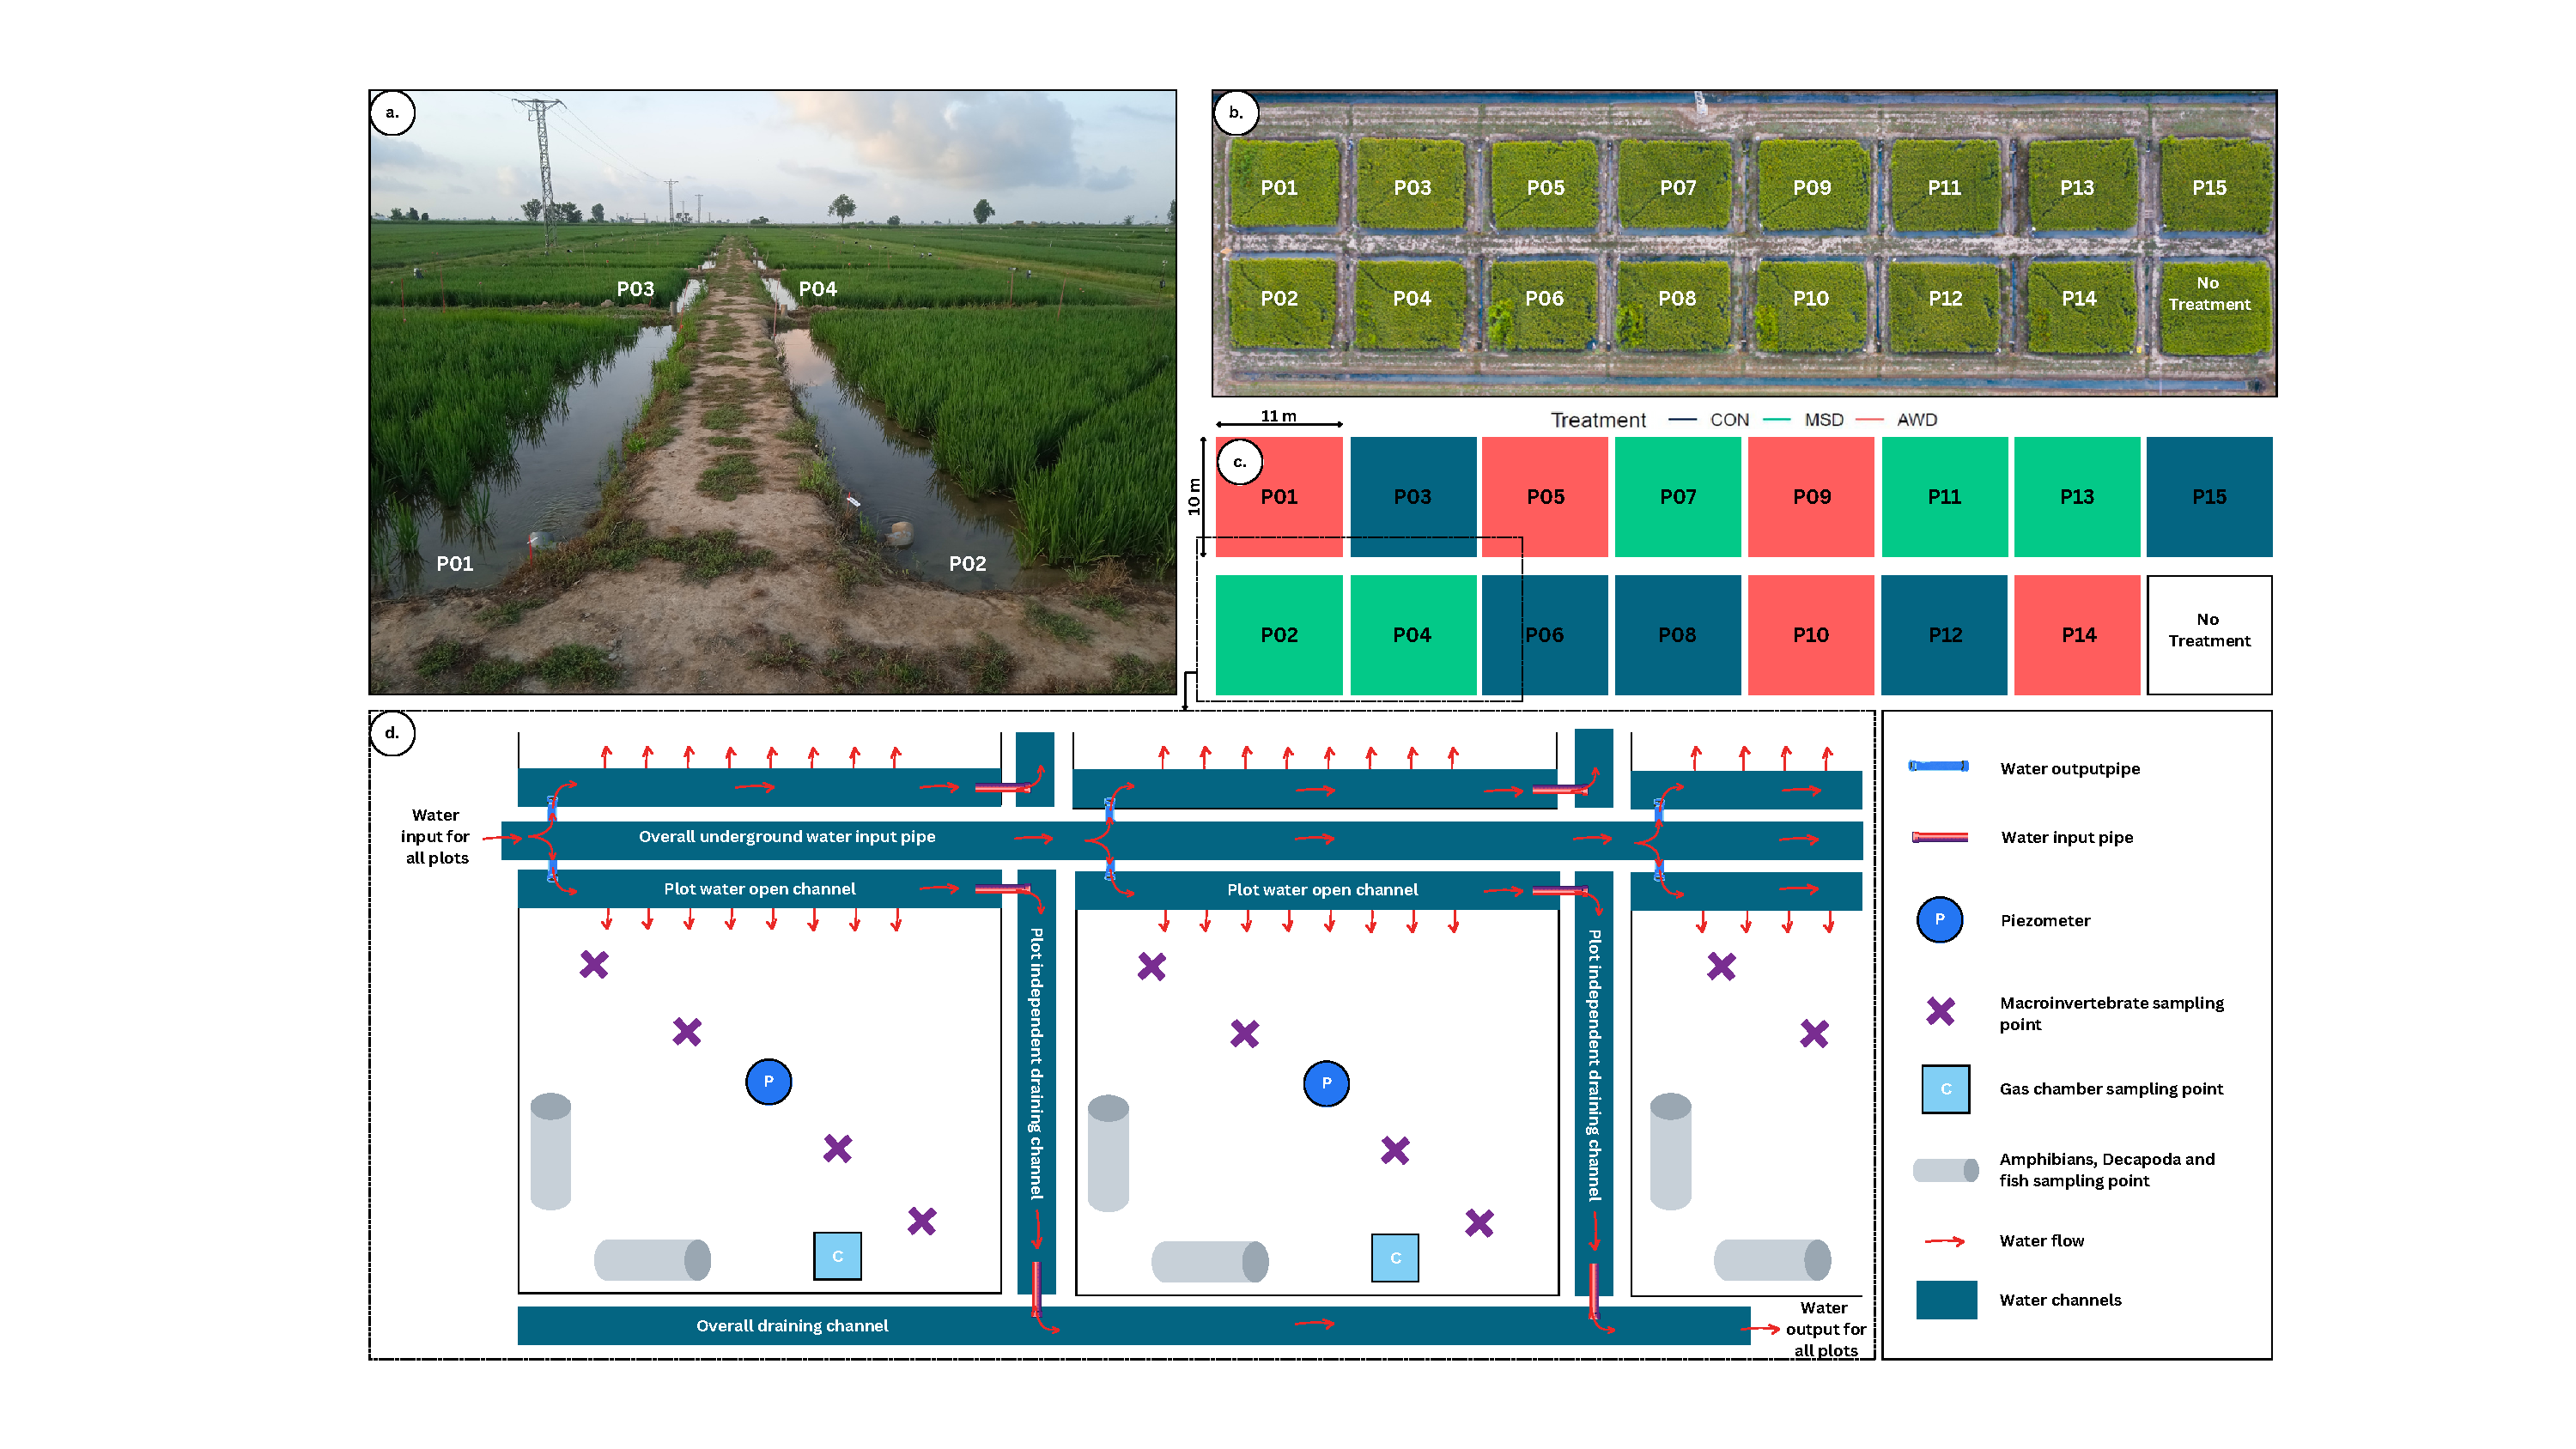
\includegraphics[scale=0.4, center]{Figures/Chapter_1/CERESTRES_layout.pdf}
	\captionof{figure}[Treats]{Experimental layout. \textbf{a.} Ground level view of experimental plots. \textbf{b.} Aerial view. \textbf{c.} Spatial distribution of water treatments. \textbf{d.} Water channelization system and sampling points within plots. Water management was independent for each plot as inputs and outputs could be opened and closed according to the assigned water strategy and thanks to each plot having its own independent draining channel on one of its sides. Piezometers, used to track water level, were installed only in MSD and AWD plots. All samplings (i.e, chambers for greenhouse gases emissions; cylindrical static nets for amphbians, decapoda and fish; and dip net sampling for macroinvertebrates) were repeated in the same location within plots for each sampling date. Abbreviations for assessed irrigation strategies stand for: CON = continuous flooding; MSD = mid-season drainage; and AWD = alternate wetting and drying.}   
	\label{Exp.lay}
\end{figure*}
%\vspace{0.5cm}\\

% CH4 alt. models example:

\begin{figure*}[htbp]
\captionsetup{justification=justified}
	\centering 
	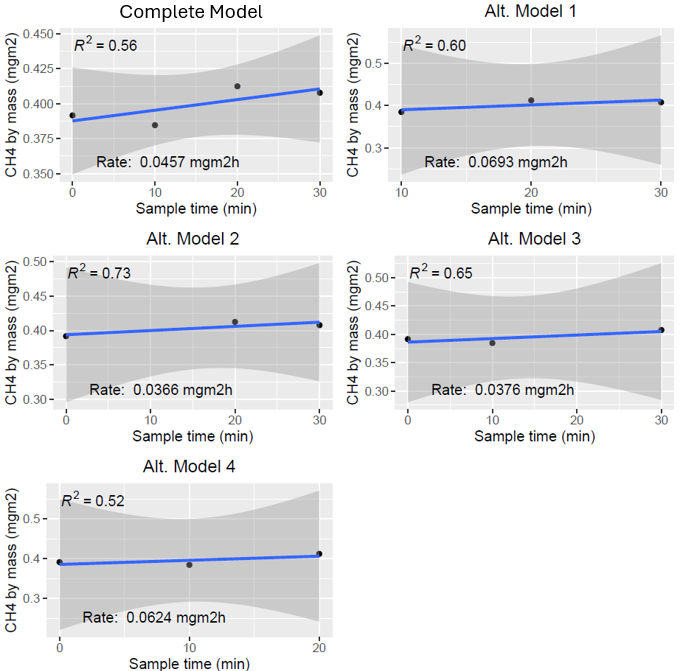
\includegraphics[scale=0.8]{Figures/Chapter_1/mod_exp.png}
	\captionof{figure}[varsTreat]{Example of alternative CH$_{4}$ flux models. The first panel (top-left) shows the complete model, with all four concentration measurements, for one sampling event. This model achieved R$^{2}$ = 0.56. The following four panels show alternative models, each dropping one of the four measurements (e.g. Alt. Model 3 drops the min=20 measurement and keeps measurements min 0; 10; and 30). For this sampling event the alternative model 2 (dropping measurement min=10) is the only one achieving R$^{2}$ $>$ 0.7, thus being considered as corrected CH$_{4}$ flux.)}  
	%\refstepcounter{SIfig}
 \label{mod_exp}
\end{figure*}

% Correlation:

\begin{figure*}[htbp]
\captionsetup{justification=justified}
	\centering 
	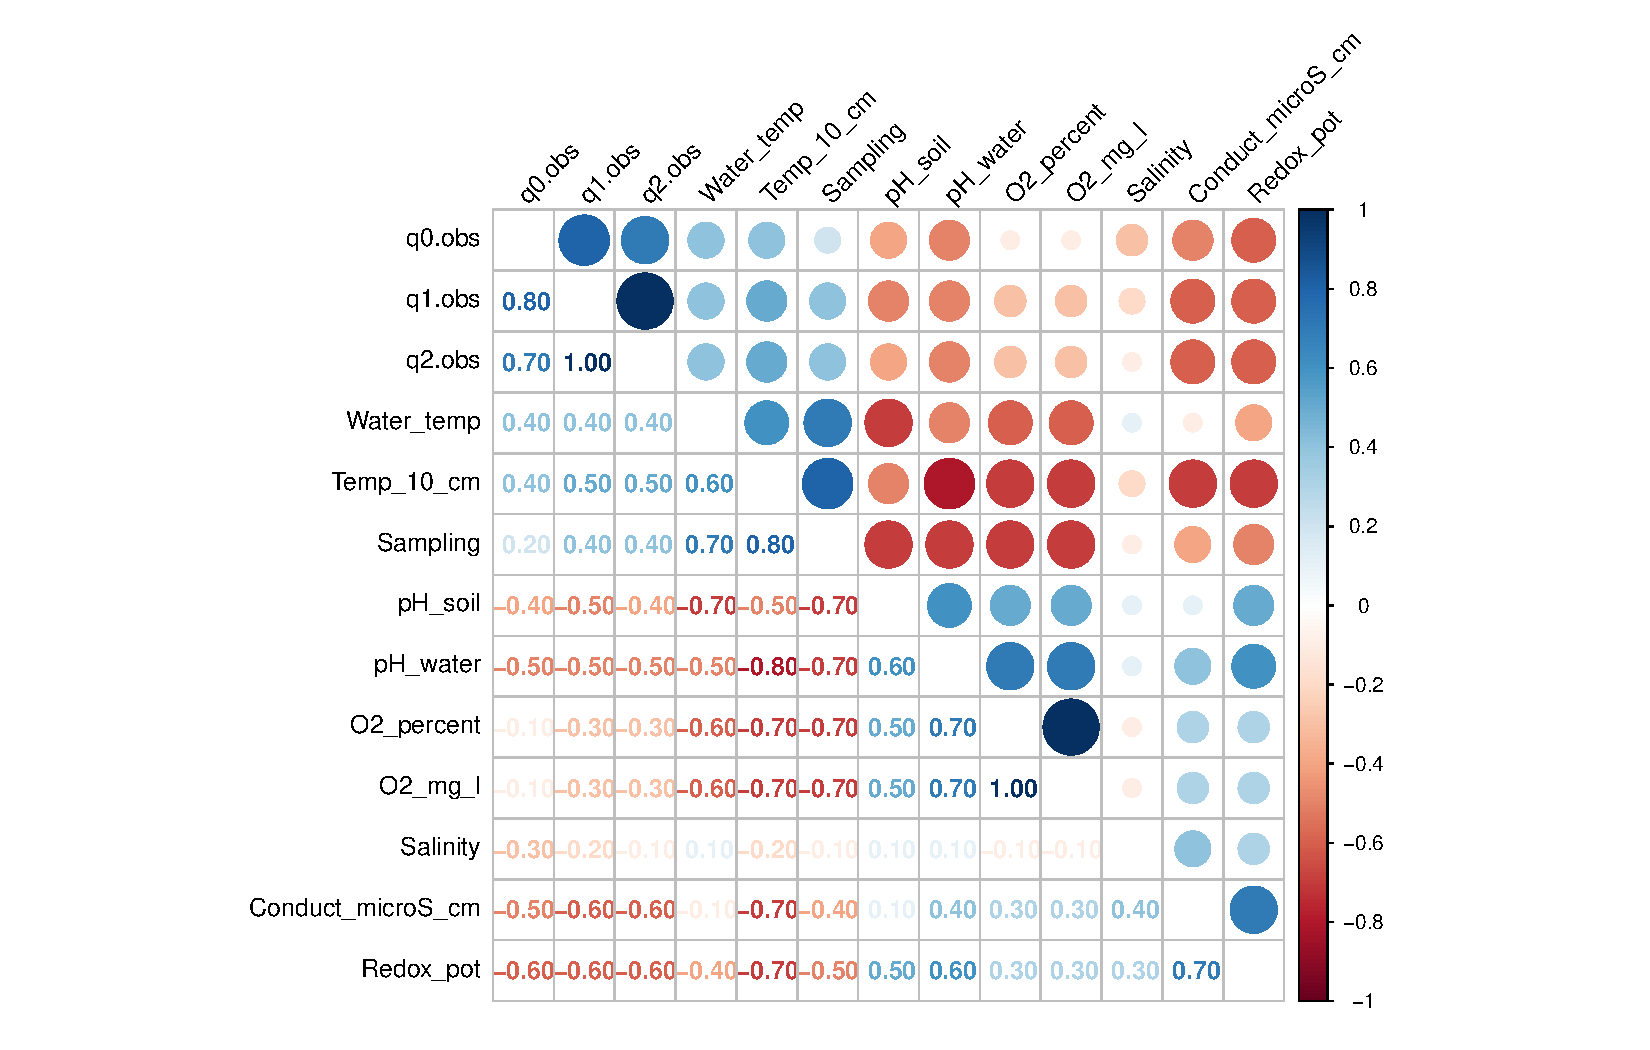
\includegraphics[scale=0.4, center]{Figures/Chapter_1/Corr_plot_nooutliers.pdf}
	\captionof{figure}[varsTreat]{Spearman's rank correlation coefficient in between soil and water physicochemical covariates, and biodiversity components (q0.obs = Species richness, q1.obs = Shannon diversity). Red circles represent negative correlation and blue circle positive correlation among variables. The size of circles is positively related to correlation among variables.}  
	%\refstepcounter{SIfig}
 \label{Corr_plot}
\end{figure*}

% Dendrogram:

\begin{figure*}[htbp]
\captionsetup{justification=justified}
	\centering 
	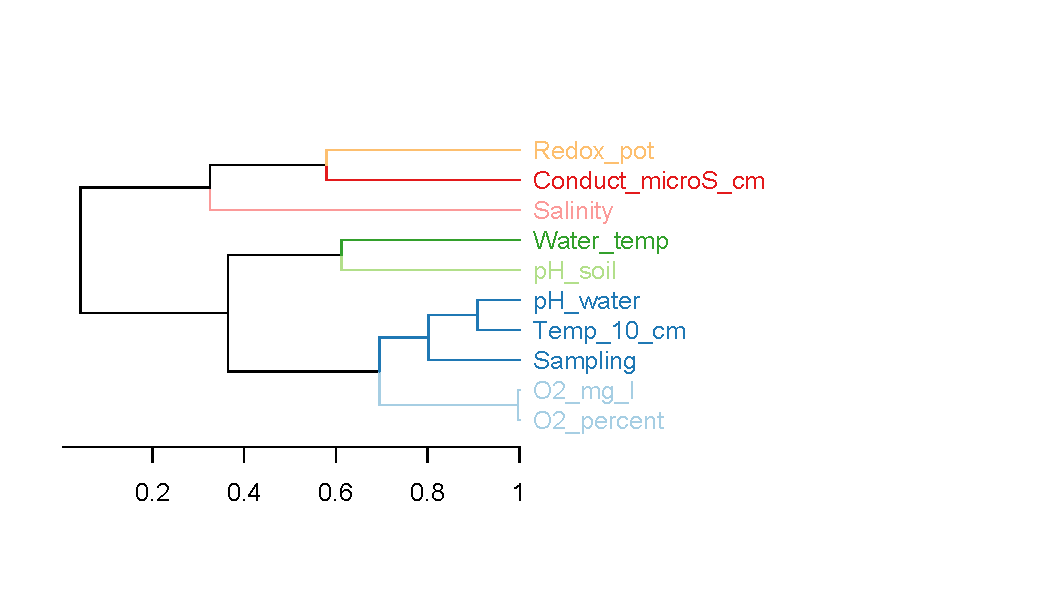
\includegraphics[scale=0.6, center]{Figures/Chapter_1/Cluster_variables_pearson_5_nooutliers2.pdf}
	\captionof{figure}[varsTreat]{Dendrogram based on the Pearson correlation coefficient for soil and water physicochemical covariates.}  
	%\refstepcounter{SIfig}
 \label{Dendro}
\end{figure*}

% Physchem variables vs Treat boxplots:

\begin{figure*}[htbp]
\captionsetup{justification=justified}
	\centering 
	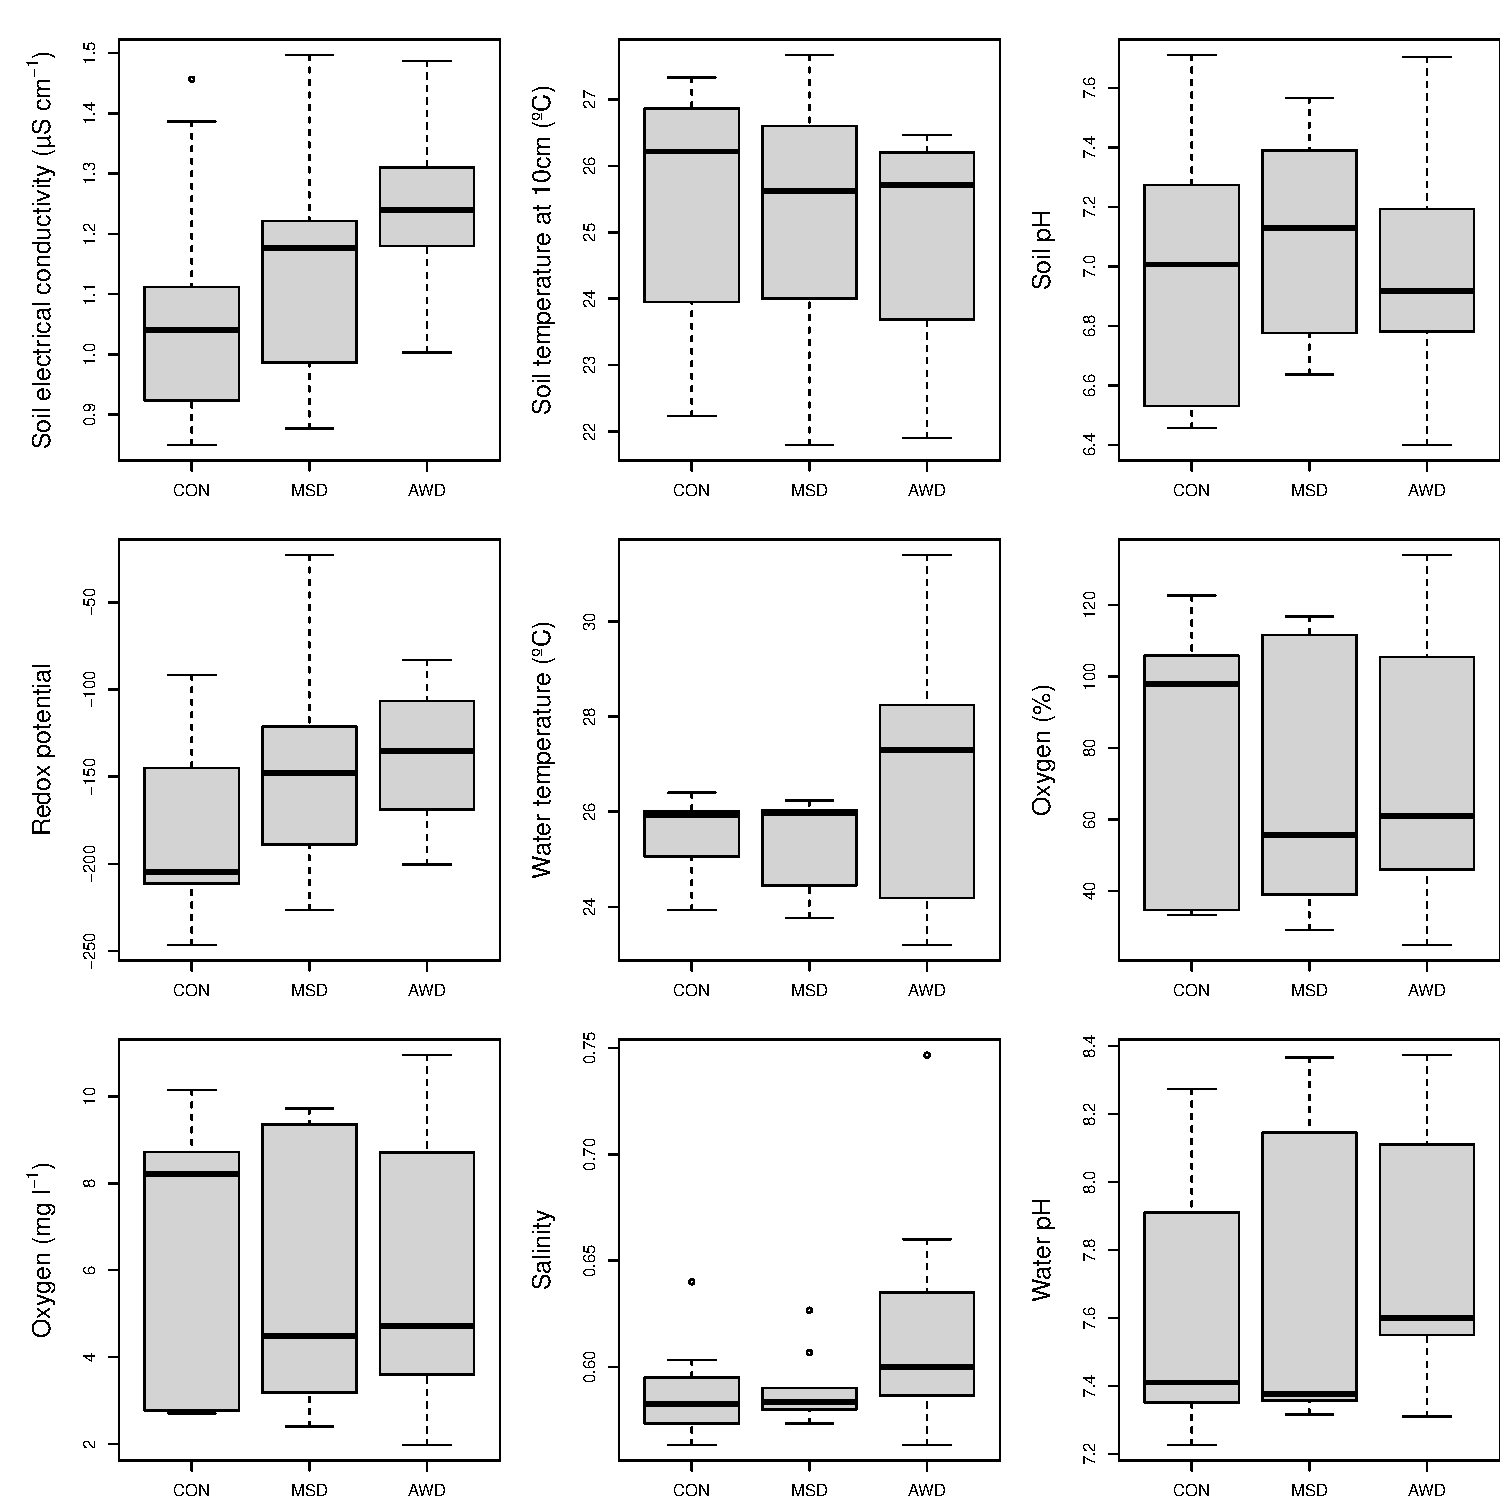
\includegraphics[scale=0.6, center]{Figures/Chapter_1/Ind_vars_Treat_inter.pdf}
	\captionof{figure}[varsTreat]{Soil and water physicochemical parameters for each water-saving irrigation strategy. Abbreviations for assessed irrigation strategies stand for: CON = continuous flooding; MSD = mid-season drainage; and AWD = alternate wetting and drying.}  
	%\refstepcounter{SIfig}
 \label{vars_Treat}
\end{figure*} 

\setcounter{table}{0}
\renewcommand{\thetable}{A.\arabic{table}} % Applies "A.1", "A.2", etc. format to appendix tables

\begin{table*} [htbp]
    \centering
    \scriptsize  
    \begin{tabular}{l | l | c c c c | c c c c | c c c c}
    \cline{1-14}
\multirow{2}{2.3cm}{Order} & \multirow{2}{3cm}{Maximum taxonomy} & \multicolumn{4}{c}{Continuous Flooding}  & \multicolumn{4}{c}{MSD} &  \multicolumn{4}{c}{AWD}  \\
    \cline{3-14}
& & S1 & S2 & S3 & S4 & S1 & S2 & S3 & S4 & S1 & S2 & S3 & S4\\
    \cline{1-14}
\multirow{6}{2.3cm}{Coleoptera}  & \textit{Enochrus  sp.} & 0 & 0 & 1 & 0 & 0 & 0 & 1 & 0 & 0 & 0 & 7 & 0\\
& Fam. Hydrophilidae & 0 & 0 & 0 & 0 & 0 & 0 & 0 & 1 & 0 & 0 & 0 & 2\\
& \textit{Helochares sp.} & 1 & 14 & 0 & 0 & 1 & 3 & 2 & 0 & 0 & 3 & 4 & 0\\
& \textit{Hydaticus  sp.} & 0 & 1 & 0 & 0 & 0 & 2 & 1 & 0 & 0 & 2 & 0 & 0\\
& \textit{Hydroglyphus sp.} & 148 & 27 & 1 & 0 & 220 & 0 & 0 & 0 & 155 & 14 & 5 & 0\\
& \textit{Rhantus suturalis} & 0 & 0 & 0 & 0 & 1 & 0 & 0 & 0 & 3 & 0 & 0 & 0\\
    \cline{1-14}
\multirow{5}{2.3cm}{Hemiptera} & \textit{Anisops sardeus} & 0 & 25 & 16 & 32 & 0 & 2 & 36 & 10 & 0 & 1 & 3 & 15\\
& \textit{Gerris sp.} & 0 & 33 & 6 & 0 & 0 & 3 & 1 & 0 & 0 & 1 & 0 & 0\\
& \textit{Mesovelia vittigera} & 0 & 17 & 2 & 2 & 0 & 7 & 2 & 4 & 0 & 0 & 1 & 2\\
& \textit{Microvelia pygmaea} & 0 & 163 & 72 & 74 & 0 & 57 & 65 & 82 & 0 & 20 & 27 & 147\\
& \textit{Sigara nigrolineata} & 17 & 25 & 9 & 1 & 16 & 1 & 25 & 0 & 5 & 7 & 0 & 6\\
    \cline{1-14}
\multirow{7}{2.3cm}{Odonata} & \textit{Coenagrion sp}. & 0 & 6 & 0 & 1 & 0 & 4 & 0 & 0 & 0 & 0 & 0 & 0\\
& Fam. Coenagrionidae & 23 & 0 & 0 & 0 & 13 & 0 & 0 & 0 & 11 & 0 & 0 & 0\\
& Fam. Libellulidae & 41 & 0 & 0 & 0 & 15 & 0 & 0 & 0 & 13 & 0 & 0 & 0\\
& \textit{Ischnura elegans} & 0 & 155 & 178 & 33 & 0 & 8 & 145 & 25 & 0 & 27 & 7 & 36\\
& \textit{Ischnura graellsii} & 0 & 9 & 37 & 13 & 0 & 0 & 0 & 6 & 0 & 0 & 0 & 24\\
& \textit{Sympetrum fonscolombii} & 0 & 14 & 4 & 0 & 0 & 0 & 0 & 0 & 0 & 0 & 3 & 0\\
& \textit{Sympetrum lefebvrii} & 0 & 2 & 0 & 0 & 0 & 0 & 0 & 0 & 0 & 0 & 0 & 0\\

    \cline{1-14}
    \end{tabular}
    \caption{Macroinvertebrate abundance in number of sampled individuals. Organisms are presented according to the maximum taxonomical resolution achieved during the identification process. Fam. and sp. indicate individuals that could be identified up to Family and Genus levels, respectively. S1 to S4 indicate each of the four macroinvertebrate samplings. Abbreviations for assessed irrigation strategies stand for: MSD = mid-season drainage; and AWD = alternate wetting and drying.}
    \label{AbuColOdoHet}
\end{table*}


\begin{table} [htbp]
    \centering
    \scriptsize  
    \begin{tabular}{l | l | c c c c c c c c }
\cline{1-10}
\multirow{2}{2.3cm}{Order} & \multirow{2}{3cm}{Species} & \multicolumn{8}{c}{Continuous Flooding} \\
    \cline{3-10}
& & S1 & S2 & S3 & S4 & S5 & S6 & S7 & S8 \\
    \cline{1-10}
Anura & \textit{Pelophylax perezi} & 0 & 89 & 25 & 1 & 0 & 0 & 0 & 0\\
    \cline{1-10}
Decapoda & \textit{Procambarus clarkii} & 3 & 28 & 27 & 112 & 188 & 248 & 152 & 118\\
    \cline{1-10}
\multirow{3}{2.3cm}{Cypriniformes} & \textit{Carassius carassius} & 3 & 0 & 1 & 0 & 0 & 0 & 0 & 0\\
  & \textit{Misgurnus anguillicaudatus} & 0 & 0 & 1 & 2 & 0 & 1 & 2 & 0\\
& \textit{Pseudorasbora parva} & 0 & 1 & 6 & 0 & 1 & 2 & 3 & 0\\
    \cline{1-10} 
\multicolumn{10}{c}{} \\
     \cline{1-10}
\multirow{2}{2.3cm}{Order} & \multirow{2}{3cm}{Species} & \multicolumn{8}{c}{MSD} \\
    \cline{3-10}
& & S1 & S2 & S3 & S4 & S5 & S6 & S7 & S8 \\
    \cline{1-10}
Anura & \textit{Pelophylax perezi} & 0 & 165 & 0 & 2 & 0 & 0 & 0 & 0\\
    \cline{1-10}
Decapoda & \textit{Procambarus clarkii} & 1 & 37 & 0 & 29 & 98 & 164 & 198 & 89\\
    \cline{1-10}
\multirow{3}{2.3cm}{Cypriniformes} & \textit{Carassius carassius} & 5 & 1 & 0 & 0 & 0 & 0 & 1 & 0\\
  & \textit{Misgurnus anguillicaudatus} & 0 & 0 & 0 & 1 & 4 & 1 & 6 & 0\\
& \textit{Pseudorasbora parva} & 0 & 1 & 0 & 1 & 1 & 4 & 6 & 1\\
    \cline{1-10} 
\multicolumn{10}{c}{} \\
     \cline{1-10}
\multirow{2}{2.3cm}{Order} & \multirow{2}{3cm}{Species} & \multicolumn{8}{c}{AWD} \\
    \cline{3-10}
& & S1 & S2 & S3 & S4 & S5 & S6 & S7 & S8 \\
    \cline{1-10}
Anura & \textit{Pelophylax perezi} & 0 & 1 & 0 & 0 & 0 & 0 & 1 & 0\\
    \cline{1-10}
Decapoda & \textit{Procambarus clarkii} & 4 & 2 & 0 & 35 & 9 & 28 & 145 & 72\\
    \cline{1-10}
\multirow{3}{2.3cm}{Cypriniformes} & \textit{Carassius carassius} & 0 & 1 & 0 & 0 & 0 & 0 & 0 & 0\\
  & \textit{Misgurnus anguillicaudatus} & 0 & 0 & 0 & 1 & 0 & 4 & 1 & 0\\
& \textit{Pseudorasbora parva} & 0 & 0 & 0 & 0 & 1 & 0 & 0 & 0\\
\cline{1-10}
    \end{tabular}
    \caption{Amphibian, decapoda and fish abundance in number of sampled individuals. S1 to S8 indicate each of the eight fortnightly samplings. Abbreviations for assessed irrigation strategies stand for: MSD = mid-season drainage; and AWD = alternate wetting and drying.}
    \label{AbuMacroFauna}
\end{table}

% Models:

\begin{table*}[htbp]
    \scriptsize % Reduce text size
    \renewcommand{\arraystretch}{0.9} % Reduce row height
    \centering
\begin{tabularx}{\textwidth}{l X}
    \toprule
Independent variable & Model\\
       \midrule 
    CH$_{4}$ emissions & CH$_{4}$ $\sim$ WS*SD + Wl + Ts + Te + Rc + C + pH+ Rx + Tw + O$_{2}$ + S + (1$\mid$Rep) \\
    Biodiversity - Species richness\_all & Sp\_all $\sim$ WS*SD + WS*SD$^2$ + C+ pH + Rx + O$_{2}$ + S + (1$\mid$Rep) \\
    Biodiversity - Species richness\_2nd & Sp\_2nd $\sim$ WS + C + pH + Rx + (1$\mid$Rep) \\
    Biodiversity - Shannon diversity & ShD $\sim$ WS*SD + WS*SD$^2$ + pH + Rx + O$_{2}$ + (1$\mid$Rep) \\
    Biodiversity - Cumulative abundance - All & Ab\_all $\sim$ WS*Order \\
    Biodiversity - Cumulative abundance - Tad & Ab\_tad $\sim$ WS; excluding AWD. \\
    \bottomrule
\end{tabularx}
    \caption{GLMM structure for each assessed independent variable. All models were built using gaussian distribution family. Abbreviations: CH$_{4}$ = Methane emissions; Sp\_all = Species richness considering all samplings; Sp\_2nd = Species richness considering only second sampling; ShD = Shannon diversity; Ab\_all = Abundance considering all orders; Ab\_tad = Abundance considering only Tadpoles; WS = Water-saving irrigation strategy; SD = Sampling Date; Wl = water level; Soil temperature; Te = Environmental temperature; Rc = Rice cover (\%); C = Soil electrical conductivity; pH = Soil pH; Rx = Redox potential; Tw = Water temperature; O$_{2}$ = Oxygen; S = Water salinity; Rep = Repetition (as random factor); Sp = Species Richness;  Order = Taxonomic orders.}
    \label{mod_str}
\end{table*}

% Model results:

\begin{table*}
    \tiny % Reduce text size
    \renewcommand{\arraystretch}{0.9} % Reduce row height
%\begin{tabularx}{\textwidth}{l X}
\begin{tabular}{l cc cc cc cc cc cc}
    \toprule
    Variable & \multicolumn{2}{c}{CH$_{4}$} & \multicolumn{2}{c}{Sp\_all} & \multicolumn{2}{c}{Sp\_2nd} & \multicolumn{2}{c}{ShD} & \multicolumn{2}{c}{Ab\_all} & \multicolumn{2}{c}{Ab\_tad} \\
    & $\chi^2$ & p-value & $\chi^2$ & p-value & $\chi^2$ & p-value & $\chi^2$ & p-value & $\chi^2$ & p-value & $\chi^2$ & p-value \\
    \midrule
    WS & 59.305 & $<$.001 & 3.576 & 0.167 & 71.575 & $<$.001 & 13.304 & 0.001 & 53.223 & $<$.001 & 0.297 & 0.586 \\
    SD & 2.690 & 0.101 & 6.599 & 0.010 & - & - & 17.607 & $<$.001 & - & - & - & - \\
    SD$^2$ & - & - & 9.976 & 0.002 & - & - & 17.378 & $<$.001 & - & - & - & - \\
    Wl & 0.010 & 0.921 & - & - & - & - & - & - & - & - & - & - \\
    Ts & 0.280 & 0.597 & - & - & - & - & - & - & - & - & - & - \\
    Te & 0.022 & 0.882 & - & - & - & - & - & - & - & - & - & - \\
    Rc & 0.393 & 0.531 & - & - & - & - & - & - & - & - & - & - \\
    C & 0.045 & 0.832 & 6.529 & 0.011 & 1.437 & 0.231 & - & - & - & - & - & - \\
    pH & 0.500 & 0.480 & 0.150 & 0.698 & 11.096 & 0.001 & 5.510 & 0.019 & - & - & - & - \\
    Rx & 0.350 & 0.554 & 0.125 & 0.724 & 3.027 & 0.082 & 0.008 & 0.930 & - & - & - & - \\
    Tw & 0.216 & 0.642 & - & - & - & - & - & - & - & - & - & - \\
    O$_{2}$ & 1.269 & 0.260 & 5.385 & 0.020 & - & - & 3.914 & 0.048 & - & - & - & - \\
    S & 0.133 & 0.716 & 0.129 & 0.720 & - & - & - & - & - & - & - & - \\
    WS*SD & 64.824 & $<$.001 & 4.540 & 0.103 & - & - & 3.064 & 0.216 & - & - & - & - \\
    WS*SD$^2$ & - & - & 6.312 & 0.043 & - & - & 2.737 & 0.254 & - & - & - & - \\
    Order & - & - & - & - & - & - & - & - & 178.842 & $<$.001 & - & - \\
    WS*Order & - & - & - & - & - & - & - & - & 46.242 & $<$.001 & - & - \\
    \bottomrule
\end{tabular}
    \caption{Model results, analysis of deviance table (Type II Wald chisquare tests). Abbreviations: CH$_{4}$ = Methane emissions; Sp\_all = Species richness considering all samplings; Sp\_2nd = Species richness considering only second sampling; ShD = Shannon diversity; Ab\_all = Abundance considering all orders; Ab\_tad = Abundance considering only Tadpoles; WS = Water-saving irrigation strategy; SD = Sampling Date; Wl = water level; Soil temperature; Te = Environmental temperature; Rc = Rice cover (\%); C = Soil electrical conductivity; pH = Soil pH; Rx = Redox potential; Tw = Water temperature; O$_{2}$ = Oxygen; S = Water salinity; Rep = Repetition (as random factor); Sp = Species Richness;  Order = Taxonomic orders.}
    \label{mod_res}
\end{table*}

% Estimated marginal means paired comparisons:

\begin{table}[htbp]
\scriptsize % Reduce text size
    \centering
    \begin{tabular}{llcccc}
        \toprule
        Variable & Pair & Estimate & Std. Err. & t-ratio & p-value \\
        \midrule
        CH$_{4}$ & AWD - CON  & -2.533  & 0.39  & -6.496  & $<$.001 \\
         & AWD - MSD  & -0.648  & 0.382 & -1.695  & 0.213 \\
         & MSD - CON  & -1.885  & 0.283 & -6.659  & $<$.001 \\
        \midrule
        Sp\_2nd & CON - MSD  & 6.683   & 0.941 & 7.100   & $<$.001 \\
         & CON - AWD  & 6.007   & 0.772 & 7.779   & $<$.001 \\
         & MSD - AWD  & -0.676  & 0.819 & -0.825  & 0.7005 \\
        \midrule
        ShD & CON - MSD  & 1.905   & 0.660 & 2.885   & 0.018 \\
         & CON - AWD  & 0.147   & 0.668 & 0.220   & 0.974 \\
         & MSD - AWD  & -1.759  & 0.692 & -2.543  & 0.040 \\
        \bottomrule
    \end{tabular}
        \caption{Results of estimated marginal means paired comparisons. Abbreviations: CH$_{4}$ = Methane emissions; Sp\_2nd = Species richness considering only second sampling; ShD = Shannon diversity.}
            \label{mod_pairs}
\end{table}

% Abundance per sampling date:

\begin{figure*}[htbp]
\captionsetup{justification=justified}
	\centering 
	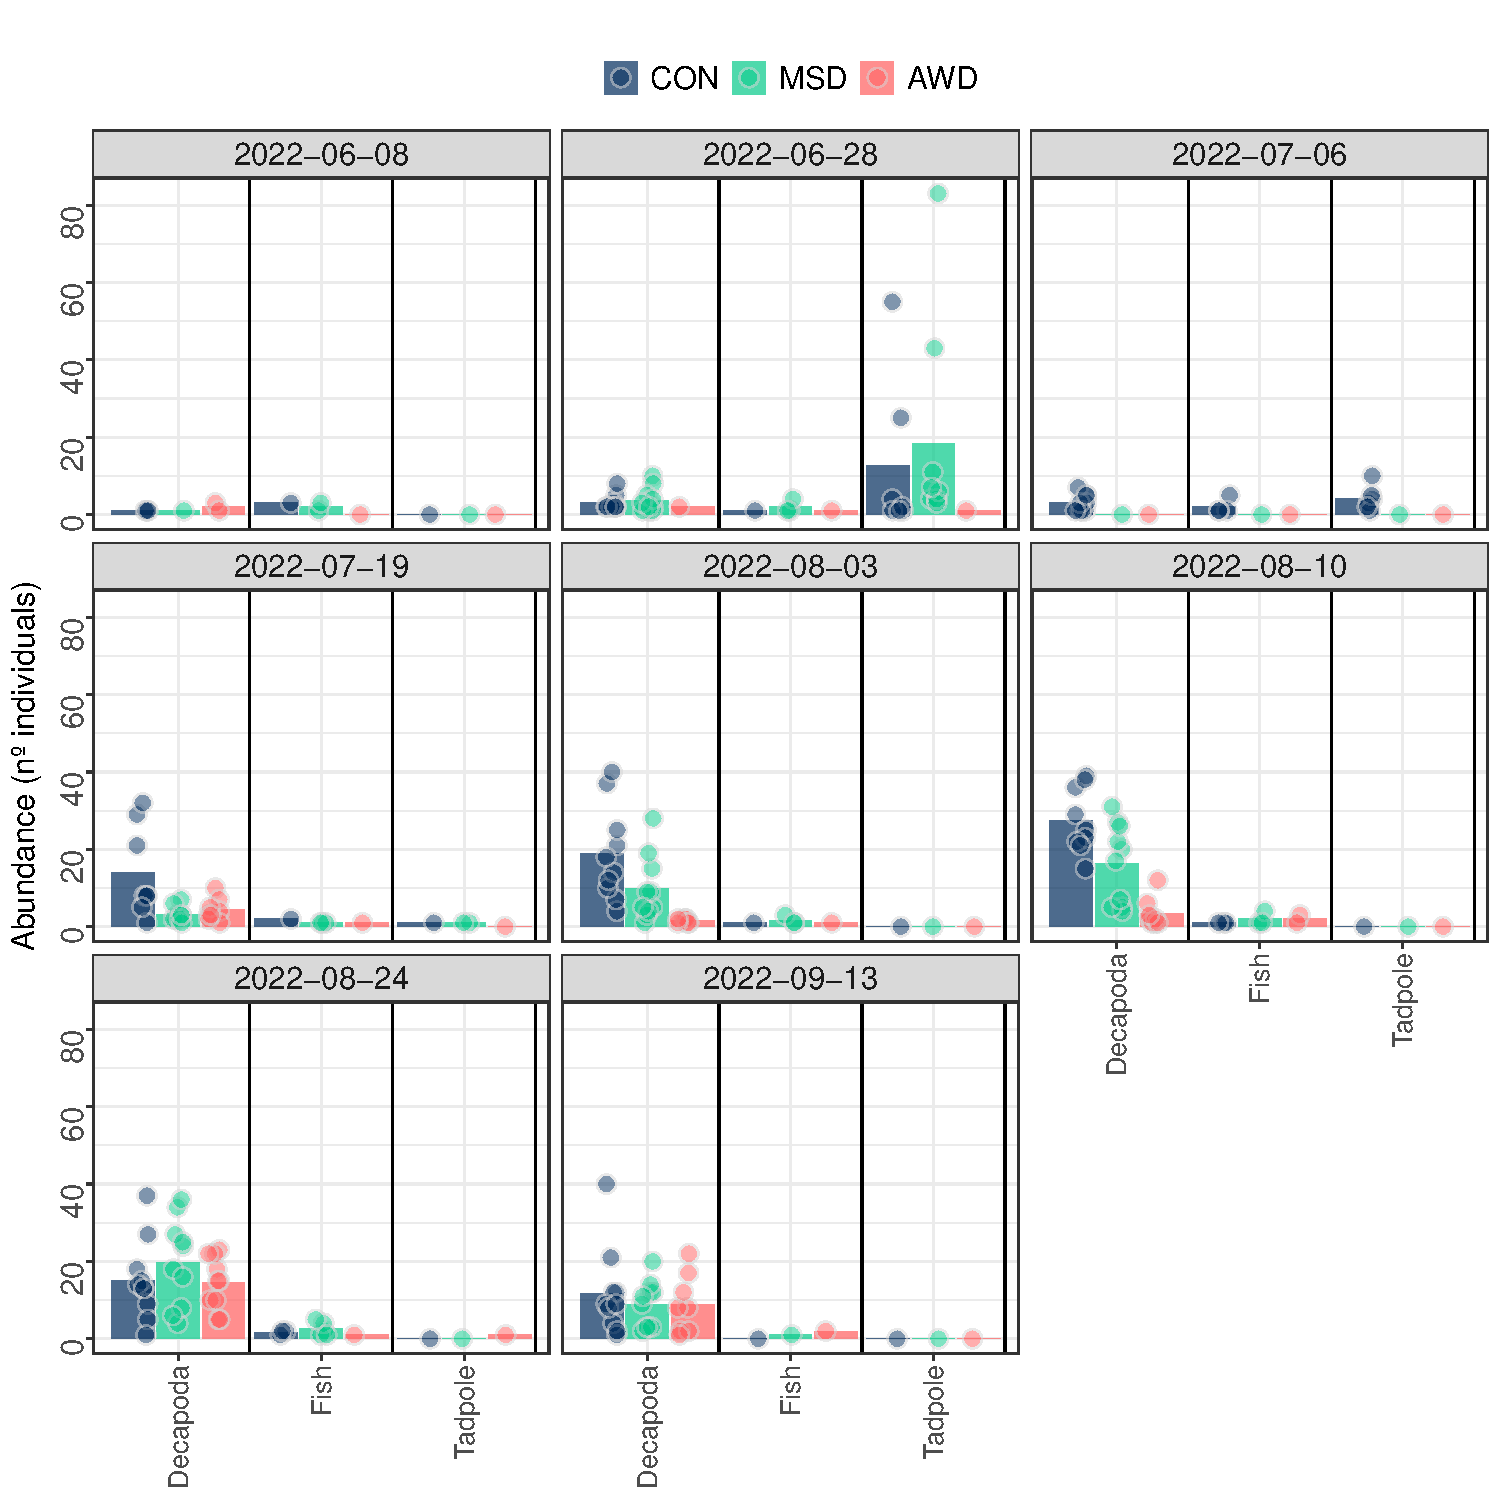
\includegraphics[scale=0.6, center]{Figures/Chapter_1/Abu.div_2022_avg_plots.perDate.pdf}
	\captionof{figure}[Abundance of aquatic communities across the growing season]{Abundance (number of individuals) of sampled aquatic vertebrate (fish and tadpoles) and red swamp crayfish communities for the three water-saving strategies across the rice growing season. Each panel shows observed abundance for a single sampling event (sampling date on top). Bars show mean abundance per irrigation strategy, while points are abundance of individuals per plot. Abbreviations for assessed irrigation strategies stand for: CON = continuous flooding; MSD = mid-season drainage; and AWD = alternate wetting and drying.}   
	\label{Abu_date}
\end{figure*}

% Restore normal figure and table numbering
\renewcommand{\thefigure}{\thechapter.\arabic{figure}}
\setcounter{figure}{0}

\renewcommand{\thetable}{\thechapter.\arabic{table}}
\setcounter{table}{0}




%\documentclass[preprint,12pt,authoryear, review]{elsarticle}
%
%\usepackage{natbib}
%\usepackage{amssymb}
%\bibliographystyle{elsarticle-harv}
%\usepackage{multirow}
%\usepackage{multicol,caption}
%\newenvironment{Figure}
%{\par\medskip\noindent\minipage{\linewidth}}
%{\endminipage\par\medskip}
%\usepackage{array}
%\newcolumntype{L}[1]{>{\raggedright\let\newline\\\arraybackslash\hspace{0pt}}m{#1}}
%\newcolumntype{C}[1]{>{\centering\let\newline\\\arraybackslash\hspace{0pt}}m{#1}}
%\newcolumntype{R}[1]{>{\raggedleft\let\newline\\\arraybackslash\hspace{0pt}}m{#1}}
%\usepackage{indentfirst}
%\usepackage{graphicx}
%\usepackage{subcaption} 
%\usepackage[export]{adjustbox}
%\usepackage{lscape} %to insert horizontal pages
%\usepackage{rotating} %to rotate elements (like tables)
%\usepackage{siunitx}
%\sisetup{round-mode=places, round-precision=2} %
%\usepackage[most]{tcolorbox} % Text boxes
%\usepackage[left=3cm,top=2.5cm,right=2cm,bottom=2.5cm]{geometry}
%\usepackage{textcomp}
%\usepackage{gensymb} %for using \mathbf{}
%\usepackage{amsbsy} % for boldsymbol{}
%\usepackage{booktabs} 
%\usepackage{lineno}
%\usepackage{tabularx} 
%\renewcommand*\footnoterule{} 
%\usepackage{reledmac}
%\usepackage{setspace}
%\usepackage{etoolbox}
%\arrangementX[A]{twocol}
%\colalignX{\justifying}
%\makeatletter
%\bhooknoteX[A]{\setstretch {\setspace@singlespace}}
%\bhookgroupX[A]{\setstretch {\setspace@singlespace}}
%\makeatother
%\let\footnote\footnoteA
%\makeatletter
%\newcommand\footnoteref[1]{\protected@xdef\@thefnmark{\ref{#1}}\@footnotemark}
%\makeatother
\def\Plus{\texttt{+}} % for personalized plus symbol
%
%\usepackage{hyperref}
%\hypersetup{colorlinks=true} 
%\urlstyle{same}
%\journal{Journal}

%\begin{document}
%
%\begin{frontmatter}

\chapter{Climate change mitigation through irrigation strategies during rice growing season is off-set in fallow season}
\label{Chapter2}

\begin{center}
\textbf{
Sebastián Echeverría-Progulakis\textsuperscript{1},
Néstor Pérez-Méndez\textsuperscript{1},
Marc Viñas\textsuperscript{2}
Mar Carreras-Sempere\textsuperscript{2}
Miriam Guivernau\textsuperscript{2}
Lluís Jornet\textsuperscript{1}
Mar Catala-Forner\textsuperscript{3}
Maite Martínez-Eixarch\textsuperscript{1}
}
\end{center}

\vspace{1ex}

\begin{center}
\textsuperscript{1} IRTA, Marine and Continental Waters Program, La Ràpita, 43540, Catalonia, Spain \\
\textsuperscript{2} IRTA, Sustainability in Biosystems Program, Caldes de Montbui, 08140, Catalonia, Spain\\
\textsuperscript{3} IRTA, Sustainable Field Crops Program, Amposta, 43870, Catalonia, Spain  \\

\end{center}


%
%
%\author[inst1,inst2, ]{Sebastián Echeverría-Progulakis}
%
%\affiliation[inst1]{organization={Marine and Continental Waters Program, IRTA},%Department and Organization
%            city={La Ràpita},
%            postcode={43540}, 
%            state={Catalonia},
%            country={Spain}}
%
%\author[inst2,b]{Néstor Pérez-Méndez}
%\author[inst3,b]{Marc Viñas}
%\author[inst3,b]{Mar Carreras-Sempere}
%\author[inst3,b]{Miriam Guivernau}
%\author[inst1,b]{Lluís Jornet}
%\author[inst2,b]{Mar Català-Forner}
%\author[inst1, ]{Maite Martínez-Eixarch}
%
%\affiliation[inst2]{organization={Sustainable Field Crops Program, IRTA},%Department and Organization 
%            city={Amposta},
%            postcode={43870}, 
%            state={Catalonia},
%            country={Spain}}
%
%\affiliation[inst3]{organization={Sustainability in Biosystems Program, IRTA},%Department and Organization 
%            city={Caldes de Montbui},
%            postcode={08140}, 
%            state={Catalonia},
%            country={Spain}}
%
%\affiliation[ ]{organization=Corresponding authors: sebastian.echeverria@irta.cat and maite.martinezeixarch@irta.cat}
%
%\affiliation[b]{organization=Contributing authors: nestor.perez@irta.cat, marc.vinas@irta.cat, mar.carreras@irta.cat, miriam.guivernau@irta.cat, lluis.jornet@irta.cat and mar.catala@irta.cat}    
     
%\doublespacing
%\begin{abstract}
\section*{Abstract}
Non-continuous flooding irrigation practices, such as alternate wetting and drying (AWD) and mid-season drainage (MSD), have been implemented in rice agroecosystems to reduce water use and mitigate climate change. Draining fields reduces methane (CH$_{4}$) emissions, as soil aeration decreases the abundance and activity of soil methanogens. Mitigation effects during the growing season have been widely studied. However, there is a knowledge gap regarding potential effects these growing season practices might have on subsequent fallow season emissions. This is relevant when assessing overall annual CH$_{4}$ emissions, particularly in systems in which fallow seasons account for a significant part of these. A field experiment was implemented in the Ebro Delta region (Catalonia, Spain) with the objective of identifying potential effects of growing season AWD and MSD on CH$_{4}$ emitted during the following flooded fallow season, in comparison to continuously flooded fields. Changes in the structure of soil microbial communities were also characterized. Both emissions and microbial communities were analyzed for rice field plots under the assessed irrigation strategies during the growing season and later for a continuously flooded mesocosm across the fallow season. Both practices achieved an average 86\% decrease in CH$_{4}$ fluxes when compared to continuous flooding during the growing season. AWD resulted in the highest fallow season emissions, leading to increases in overall annual cumulative CH$_{4}$ emissions (\Plus 8\%), global warming potential (\Plus 30\%) and yield-scaled global warming potential (\Plus 70\%) compared to continuous flooding. Growing season AWD decreased the relative abundance of both methanogens and methanotrophs in the fallow season. Reduced methanotroph communities might lead to lower CH$_{4}$ consumption, resulting in higher fallow season emissions and offsetting the mitigation effect achieved during the growing season. Under the studied conditions, MSD represented a more effective mitigation strategy. These results highlight the importance of considering both rice growing and fallow season when assessing climate change mitigation strategies.\\ 

%\end{abstract}

%\begin{keyword}
%% keywords here, in the form: keyword \sep keyword
\noindent\textbf{Keywords:}Greenhouse gas emissions; paddy rice; water management; legacy effects; soil microbiology 

%\end{keyword}

%\end{frontmatter}

%\linenumbers

%\doublespacing

\section{Introduction}
\label{sec:intro}

% PAR 1: Rice and its importance in food security and GHG emissions

Rice (\textit{Oryza sativa L.}) is a major staple crop and the third largest harvested area worldwide, accounting for approximately 11\% of total arable land \citep{Faostat2022}. Besides its critical role as food source, paddy rice cultivation is also a key anthropogenic driver of greenhouse gas (GHG) emissions \citep{bouman2007rice, nabuurs2022agriculture}. Most rice systems are managed under continuous flooding during a major part of the growing season, leading to high methane (CH$_{4}$) emissions due to favored anaerobic metabolic pathways within soil microbial communities \citep{conrad2007microbial, perry2024}. When paddy fields are drained, higher oxygen availability in soils promotes nitrous oxide (N$_{2}$O) production and emission \citep{cai1997methane}. Both CH$_{4}$ and N$_{2}$O are among the three most important GHG in the atmosphere, after CO$_{2}$, and contribute 27 and 273 times more, respectively, to global warming potential (GWP) than CO$_{2}$ at a 100 year time horizon \citep{IPCC2021}. Overall, rice production accounts for 11\% of total anthropogenic emissions of these non-CO$_{2}$ emissions \citep{Smith2007}.\\ 

% PAR 2: Context of flooded fallow (as suggested by Reviewer #4):

Winter flooded fallow season is a practice restricted to particular rice production areas, such as in the US (e.g. California, \cite{fitzgerald2000}; Arkansas, \cite{reba2019}), China (12\% of total cultivated area, \cite{zhang2011}), Spain and some reduced areas in southern France and northern Italy \citep{pernollet2015}. This practice has been promoted by policies aiming at enhancing waterbird habitat creation \citep{elphick2010, tajiri2013effects}, replacing straw burning practices (i.e., by increasing incorporated straw decomposition rates), and due to several other agronomic benefits (e.g. limiting erosion, inhibiting weed seed germination and retaining sediments and nutrients; \cite{negri2020}). In the Ebro Delta (Catalonia, Spain) rice production region, keeping fields flooded during winter is a common practice to improve straw decomposition but mainly to preserve its status of biodiversity hotspot \citep{day2006, perez-mendez2022}. Flooding fallow fields, nevertheless, increases both winter and subsequent growing season CH$_{4}$ emissions in comparison to drained fallow fields \citep{cai2000}. In flooded fallow rice systems, decreased rates of straw input and nitrogen fertilization  have been found to decrease fallow CH$_{4}$ emissions \citep{martinez-eixarch2021a}. Furthermore, positive effects of field drains during previous growing seasons have been identified to extent into fallow season emissions \citep{martinez-eixarch2022}, but there is still a lack of studies comparing the effect of different irrigation strategies on overall annual emissions.\\

% PAR 3: Alternative water managements to permanent flooding as effective CH4 mitigation measures

Awareness of rice contribution to climate change is driving an increase in research efforts to develop adaptation and mitigation strategies in its production \citep{alexandratos2012world, zhang2018effect, hussain2020rice}. Rice irrigation practices involving drainage conditions, such as alternate wetting and drying (AWD), consisting of several flooding-drainage cycles through the growing season, and mid-season drainage (MSD), with just one drain event in the season, have been largely studied and implemented \citep{li2004, li2014, lampayan2015}. The principle behind these strategies is that introducing aerobic conditions to soils inhibits the activity of anaerobic methanogenic archaea, thus reducing CH$_{4}$ emissions \citep{kumar2019alternate, perry2024}. Whereas these practices are effective in reducing emissions by 53\% on average during the growing season \citep{jiang2019water}, little is known about how their effects extend into subsequent flooded fallow seasons, which in temperate production areas can account up to 70\% of overall annual emissions \citep{martinez2018neglecting}. Draining events during the growing season might, for instance, drive long lasting changes in the activity and composition of microbial communities that can be extended to the fallow season, ultimately affecting overall emission outcomes. \\

% PAR 4 - after Reviewer's #4 suggestion: Legacy effects

Impacts that previous conditions might have on current processes and properties, have been termed as legacy effects, a concept that has been applied in the context of climate change to describe how ecological legacies result from feedbacks between biotic, soil, and geomorphic processes \citep{monger2015legacy}. Legacy effects of previous land and water management in rice paddy fields on soil organic matter content, structures of soil microbial communities and, therefore, CH$_{4}$ and N$_{2}$O emissions have been identified \citep{shao2017, tian2022}. Characterizing the main factors driving such effects is crucial to understanding potential outcomes of implementing mitigation practices. On one hand, constant high soil carbon inputs through straw incorporation after each year rice harvest correlates positively to incremental CH$_{4}$ emissions, up to a threshold of CH$_{4}$ production is reached \citep{hatala2012}. On the other, long term continuous flooding management increases the abundance of soil methanogens and CH$_{4}$ emissions, compared with soils under non-continuous flooding practices, due to a progressive adaptation of microbial communities to irrigation management \citep{lagomarsino2016a}.\\

% PAR 5  - after Reviewer's #4 suggestion: Our hypothesis

In this context, this study was set to determine potential legacy effects of water management practices implemented during the rice growing season on CH$_{4}$ emissions during a flooded fallow season. During the previous season (2022), AWD resulted in 12,9\% grain yield decrease versus continuously flooded plots. Similar decreases in current yields would probably mean a decrease in carbon inputs, due to less biomass produced and less straw incorporated. Additionally, MSD had previously been identified as a practice with mitigation effects lagging onto the fallow season in the studied site \citep{martinez-eixarch2022}. Such background supported the hypothesis of non-continuous flooding strategies maintaining their positive climate mitigation effect into the fallow season, through a decrease in CH$_{4}$ emissions, led by decreased carbon inputs and lower methanogen abundance than in microbial communities adapted to continuous flooding conditions. To test this hypothesis we specifically characterized the following issues across the three assessed irrigation strategies: i) CH$_{4}$ emission patterns during both growing and fallow season, ii) GWP and yield scaled global warming potential (GWPY), iii) microbial community composition during both periods, and iv) relative abundance of microbial functional groups related to CH$_{4}$ metabolism (i.e., methanogens and methanotrophs) during the flooded fallow season.\\

\section{Materials and methods}
\label{sec:meth}

\subsection{Study site}
\label{sec:meth_Site}

Experiments were set within the IRTA Ebro Experimental Station facilities in Amposta, Ebro Delta, Catalonia, Spain (40°42’88 30.2” N, 0°37’ 56.5” E). This deltaic region covers a surface of 320 km$^2$, where natural ecosystems contrast with rice paddy fields, which dominate the overall landscape \citep{romagosa2013sustainability}. Around 210 km$^2$ are managed as rice fields, accounting for 65\% of the total surface. The conventional local practice is to keep these fields under continuous flooding for most of the growing season (May to early October). During the fallow season subsequent to rice harvest (October to December), the remaining straw is chopped and incorporated before winter flooding \citep{martinez-eixarch2021a}. Flooding and draining large surfaces of paddy fields is accomplished thanks to a complex channel network transporting freshwater from the Ebro river. These irrigation practices require a constant input of large volumes of freshwater, and this high water demand is in conflict with current regional water availability. The Meteorological Service of Catalonia declared the current drought as the worst in record, being 2023 the second-driest year, only after 2022 \citep{MeteoCat2024}. 

\subsection{Experimental layout}
\label{sec:meth_Exp}

During the 2022 and 2023 rice growing and fallow seasons, a field experiment was conducted to assess the effect of water irrigation strategies implemented during growing seasons on GHG emissions during a flooded fallow season. Crop and water management was similar across both years. All samplings and results in this study correspond to the second year of this experiment (2023), representing, therefore, the cumulative effect of two growing seasons of water irrigation strategies on this second year fallow season. All growing season CH$_{4}$ emission (fluxes and cumulative), GWP, GWPY and grain yield presented results correspond as well to the second year of this experiment. The experiment consisted of 15 paddy rice plots of $10 \times 11$ m each. These were distributed in five blocks, each with three plots randomly assigned to one of three assessed irrigation strategies (experimental treatments): (i) conventional continuous flooding (CON), in which plots were kept flooded through the entire growing season; (ii) mid-season drainage (MSD), consisting on a single 11-days drain event before panicle initiation (June 22$^{nd}$ to July 3$^{rd}$); and (iii) alternate wetting and drying (AWD), strategy in which plots are flooded and drained cyclically through the growing season starting from 4-leaf stage (June 8$^{th}$) onwards (Figure \ref{treat}; Table \ref{field_mgmt}). Individual drainage channels were set up for each plot, allowing independent water management. All plots were water seeded at a rate of 500 seeds m$^{-2}$. To avoid strong yield declines, AWD plots were kept flooded in between heading and the end of flowering (July 3$^{rd}$-25$^{th}$) and managed under the Safe-AWD protocol \citep{bouman2007a}, setting 15 cm below ground level as water level threshold triggering plot re-flooding. Fertilization was carried out through the application of a granulated controlled-released fertilizer (33\% N, 9\% P, 6\% K) on a dose of 190 kg ha$^{-1}$. All plots were drained for three days (June 27$^{th}$-29$^{th}$) due to an herbicide and fungicide application and then later in the season, 20 days before harvest, to allow harvester access. All plots were seeded with JSendra, a commercial round rice variety predominant in the Ebro Delta area. Soil texture at the study site is silty clay (49.3\% clay; 43.8\% silt; 6.9\% sand). For a detailed description of soil physicochemical properties and nutrient content see Table \ref{straw} (containing soil analysis results from a sample composed of sub-samples from all 15 field plots).\\ 

\begin{figure} [ht]
\captionsetup{justification=justified}
	\centering 
	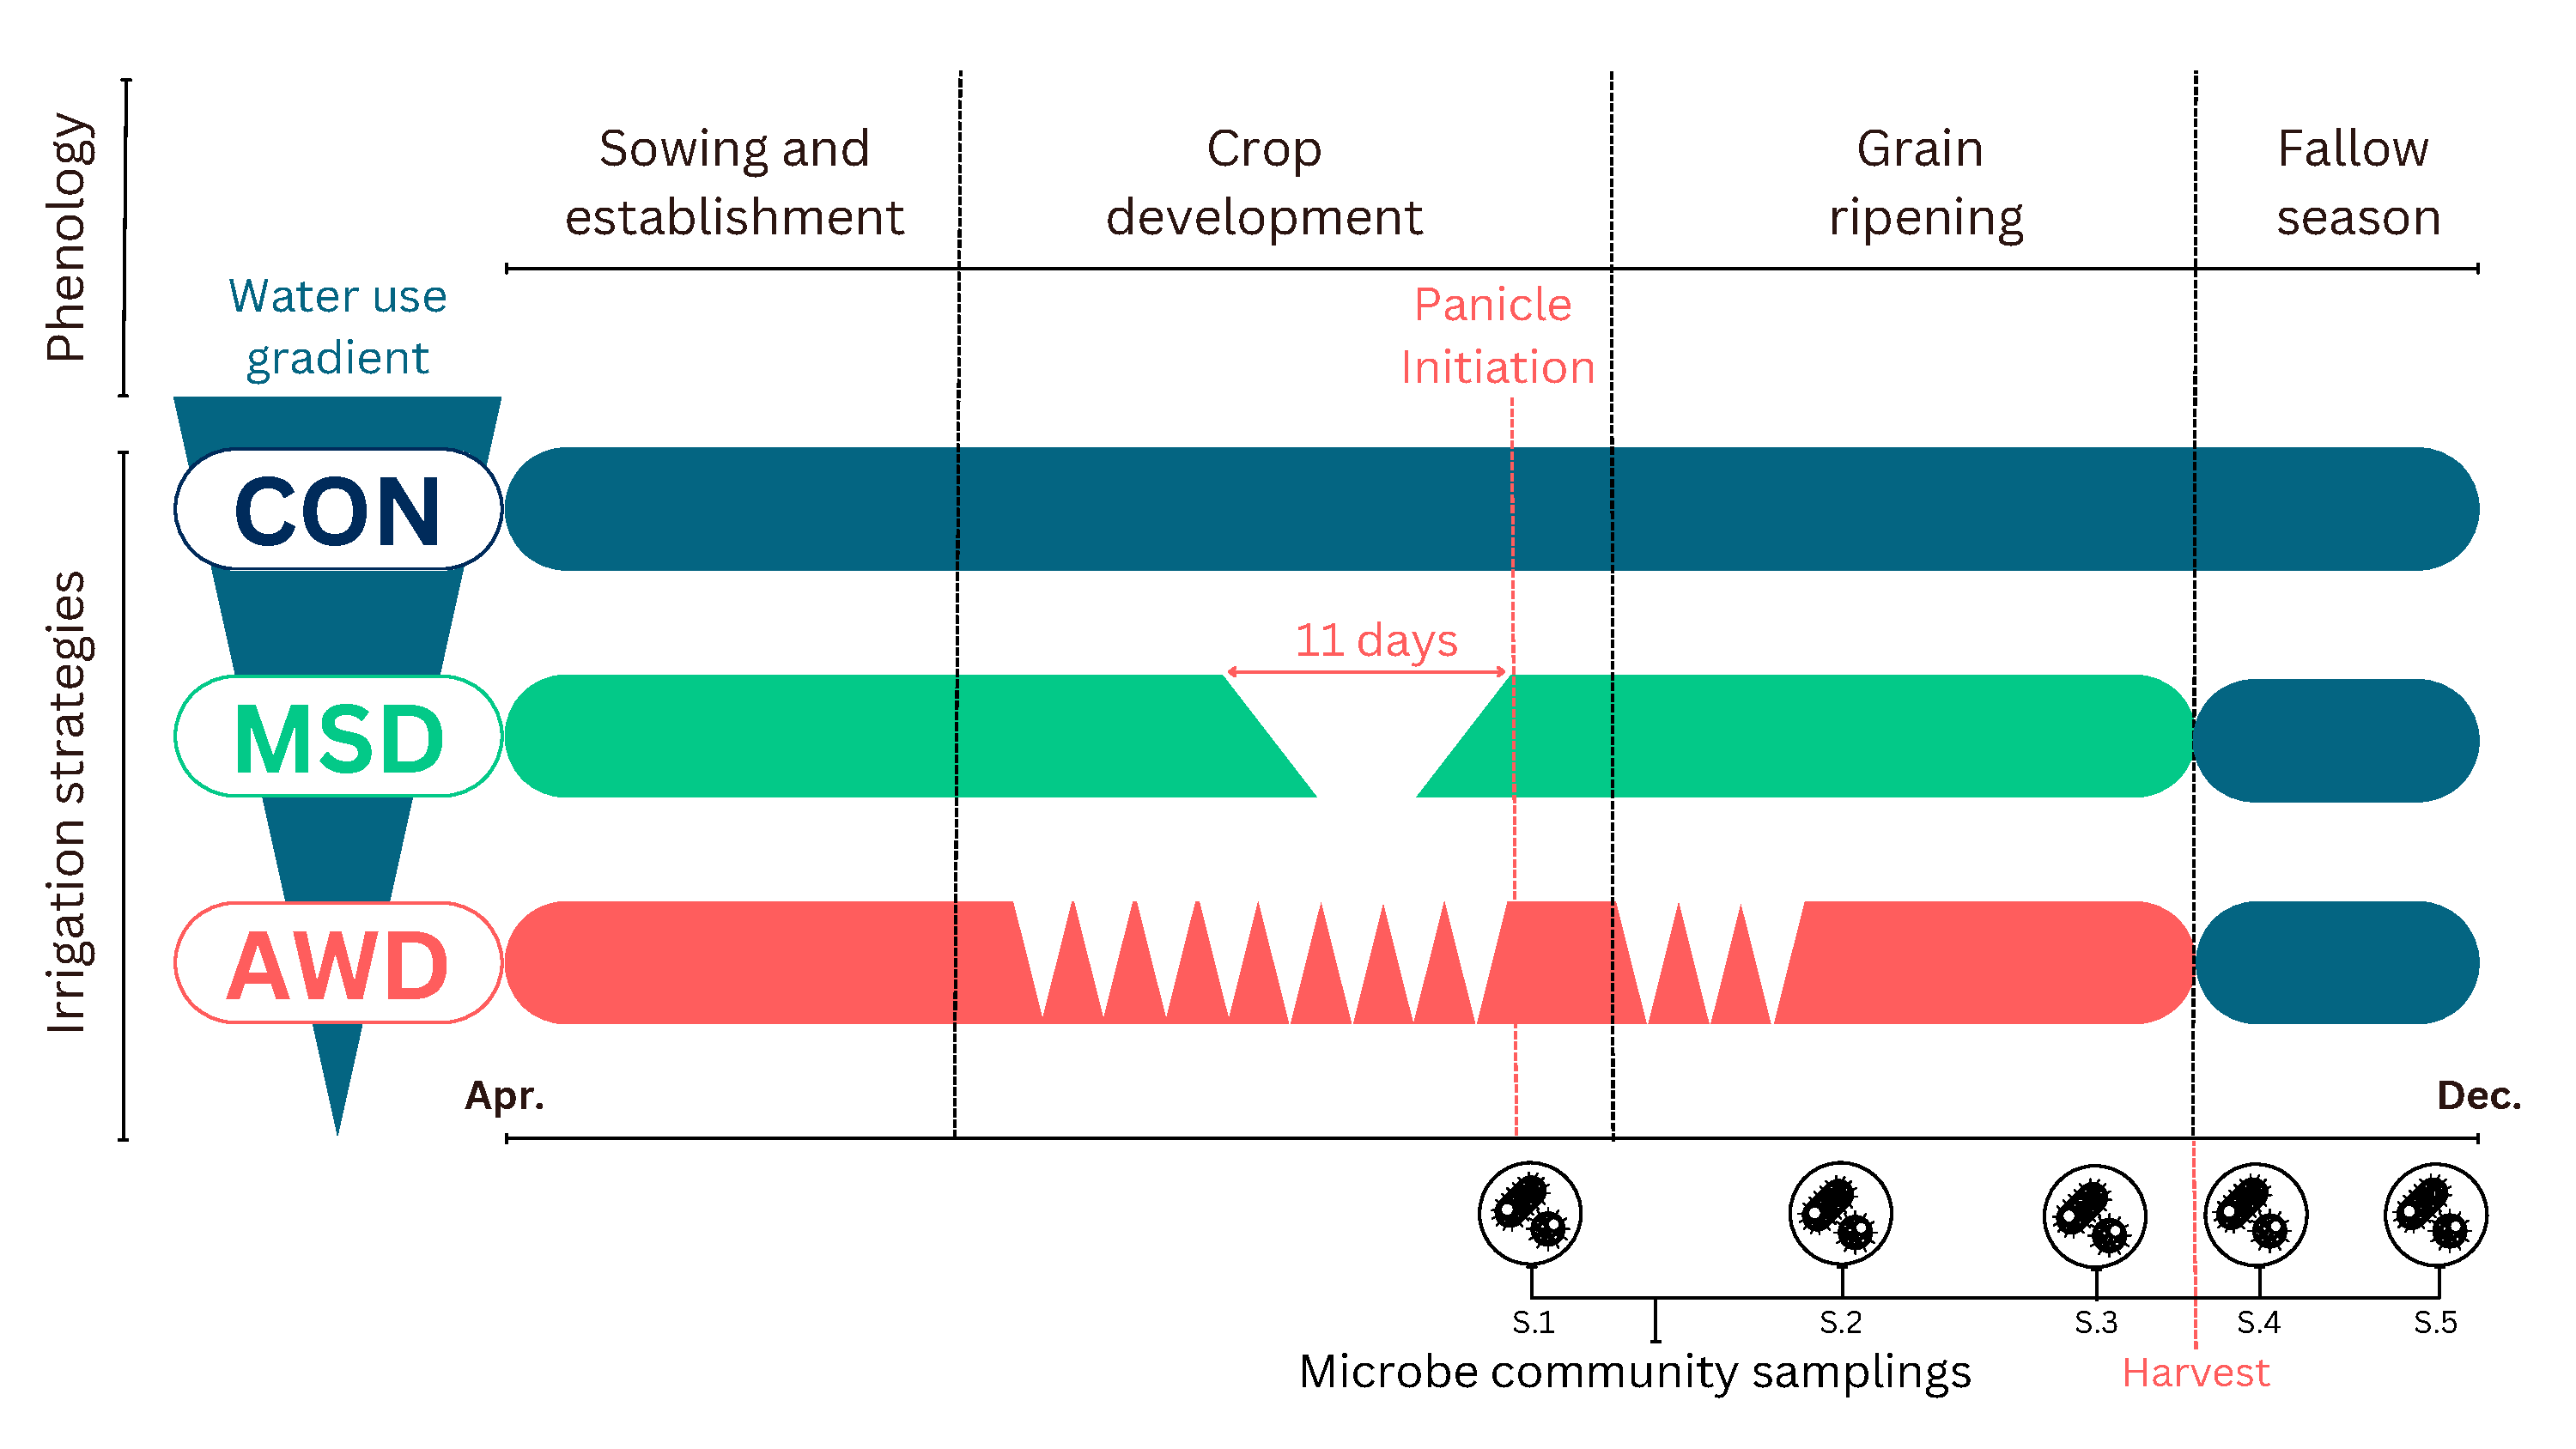
\includegraphics[scale=0.3, center]{Figures/Chapter_2/CERESTRES_Layout_2023_GSFS.pdf}
	\captionof{figure}[lay]{Assessed irrigation strategies. Horizontal bars represent the water layer for each assessed irrigation strategy across a decreasing water use gradient: conventional continuous flooding (CON); mid-season drainage (MSD); and alternate wetting and drying (AWD). Strategies are depicted for phenological stages across the growing season. The fallow season corresponds to continuous flooding for all plots. Microbe community samplings (S.1 to S.5) are shown in reference to the corresponding date and water treatment period in which they were collected: growing season (S.1, S.2 and S.3); and fallow season (S.4 and S.5).}
	\label{treat}
\end{figure}
%\vspace{0.5cm}

As an adaptation practice towards current severe droughts in the region, water available for irrigation in agriculture was halved throughout rice growing season by the local water administration. Blocking connections between main and individual plot input channels, plus keeping high water levels in individual plot drainage channels, allowed us securing continuous flooding and avoided unscheduled plot drains during main channel cuts due to this regional measure. These practices minimized potential negative effects drought might have caused on the representability of our study. Similar emission rates and trends to those registered in previous studies within the same site confirm this \citep{martinez-eixarch2021a}. A potential stop in irrigation water inflows after harvest meant risking the fallow season section of this study as field plots would have been left out of water inputs to maintain them flooded. To avoid this, the fallow season experimental layout was modified from field plots into a mesocosm experiment. The same day field plots were harvested (October 3$^{rd}$), rice plants located in a $50 \times 50$ cm frame for each plot, in which non-steady GHG sampling chambers had been installed during the growing season (see section \ref{sec:meth_GHG}), were hand harvested and grains were stored to be then added to each plot final yield. Straw residues from plants harvested within these frames were sun dried for 72 hours and chopped into 10 cm sections, emulating local open air straw drying periods and post-harvest mechanized chopping practice. After hand harvest, soil from these frames was removed down to 18 cm deep, placed within plastic boxes (54 $\times$ 48 $\times$ 37 cm, from now referred as mesocosm units), labeled according to its corresponding original field plot, and saturated with water. After three days, collected and sun dried straw was weighed to determine dry weight and incorporated by hand to each box. All irrigation strategies resulted in similar aboveground biomass, thus similar amounts of straw were incorporated to all mesocosm units (Table \ref{straw}). Soil boxes were then flooded up to 5 cm above soil level and kept flooded to this level all through the fallow season (Figure \ref{meso}). Wetland soil mesocosm experiments have proven a controlled, practical and representative methodology in previous wetland research on the fields of GHG emissions \citep{capooci2019experimental} and structure of soil microbial communities \citep{donato2020nitrogen}. Mesocosm unit representativeness of field plot soil conditions was assessed comparing physicochemical parameters with field measurements from previous flooded fallow seasons in the same experimental station (same soil texture). All assessed parameters in mesocosm units varied within similar ranges and behaved through the fallow season accordingly to previous field measurements (Figure \ref{meso_field}). \\

\begin{table*} [htbp]
    \centering
    \footnotesize  
    \begin{tabular}{ l  l  l }
\cline{1-3}
{Season} & {Date} & {Management} \\
\cline{1-3}
\rule{0pt}{3ex} % inserts space
{Growing} & {25-Apr-23} & {Fertilization (granulated controlled-release; NPK=33-9-6; 190 kg ha$^{-1}$)} \\
{} & {30-Apr-23} & {Flooding (all plots)} \\
{} & {02-May-23} & {Sowing (var. JSendra; 500 seeds m$^{-2}$)} \\
{} & {18-May-23} & {Herbicide treatment (Clincher)} \\
{} & {08-Jun-23} & {Start of first drain-flood cycle in  AWD plots} \\
{} & {22-Jun-23} & {MSD plots drained} \\
{} & {28-Jun-23} & {Herbicide treatment (Logan + Kaos)} \\
{} & {03-Jul-23} & {MSD plots re-flooded; end of first drain-flood cycles in  AWD plots} \\
{} & {25-Jul-23} & {Start of second drain-flood cycle in  AWD plots} \\
{} & {31-Jul-23} & {Fungicide treatment (Trifloxystrobin)} \\
{} & {11-Aug-23} & {End of second drain-flood cycles in  AWD plots} \\
{} & {15-Sep-23} & {Final drain (all plots)} \\
\rule{0pt}{3ex}
{Fallow} & {03-Oct-23} & {Harvest; hand harvest of frames for mesocosm setup; filling of mesocosm units} \\
{} & {06-Oct-23} & {Straw integrated to mesocosm units; flooding of mesocosm units}\\
\cline{1-3}
    \end{tabular}
    \caption{Crop treatments, experimental setup and irrigation management schedule.}
    \label{field_mgmt}
\end{table*} 

\subsection{Greenhouse gas flux measurement}
\label{sec:meth_GHG} 

For both growing and fallow seasons, GHG emissions were sampled weekly according to the non-steady chamber method, adapted from \cite{martinez2018neglecting}. Due to time and logistic constraints regarding the need of simultaneous sampling for data comparability, GHG emission samples were collected from three of the five experimental blocks throughout both growing and fallow seasons. Sample collection was done always on the same three blocks. 
% removed after Reviewer #4's suggestions: For each sample date, four 30 ml gas samples were taken every 10 minutes over a 30 minutes sampling period from each chamber using syringes. Sampled air was then transported into pre-evacuated 12.5 ml glass vials (Labco Ltd., Buckinghamsire, UK). Samplings were made in between 09:00 and 14:00 to minimize variability from daily GHG emission curves. Gas samples were then analysed in laboratory to determine GHG concentrations using a THERMO TRACE 2000 (Thermo Fisher Scientific, USA) gas chromatograph equipped with a flame ionization detector (FID, Trace GC 2000, Thermo Finnigan, Germany). 
For each sampling date, soil (electrical conductivity, temperature, redox potential and pH; all measured at 10 cm-depth) and water (temperature, salinity, oxygen concentration, oxygen saturation and pH) physicochemical parameters were registered. These parameters were assessed using an automated YSI Professional Plus (Pro Plus) Multiparameter Instrument (Brannum Lane, USA), a Hanna Instruments HI 98190 pH/ORP pH-meter and a Fieldscout direct soil E.C. meter (Spectrum Technologies, 2019). Additionally, GWP and GWPY were calculated for each irrigation strategy and rice season according to the \cite{IPCC2021} guidelines. Yield was recorded from final field plots harvest in Mg ha$^{-1}$ at 14\% humidity.\\

\subsection{Microbial biodiversity assessment}
\label{sec:meth_BIO}

Soil cores were collected from all field plots and mesocosm units to characterize microbial communities and their dynamics. A total of five soil sampling events were conducted, three during  the growing season and two during the fallow season. Growing season samplings were done after MSD drainage and first period of AWD cycles (Figure \ref{treat}, microbe community sampling S.1, July 5$^{th}$); after the second period of AWD cycles (S.2, August 16$^{th}$); and before harvest (S.3, September 5$^{th}$). During the fallow season, samplings were carried out a week after harvest, three days after straw incorporation (S.4, October 11$^{th}$); and during mid fallow season, 31 days after straw incorporation (S.5, November 6$^{th}$). \\
% removed after Reviewer #4's suggestions: During the growing season samplings, three cores were collected from each field plot, whereas only one core was collected per mesocosm unit during the two fallow season samplings. From all collected cores across seasons, top (0 to 3 cm) and bottom (5 to 10 cm) sub-samples were collected. The three top sub-samples collected per plot during the growing season were merged together, the same procedure was repeated for bottom sub-samples, obtaining one top and one bottom merged sub-sample per plot. These sub-samples were collected in 1.5 mL sterile tubes and transported to the lab at -4 \degree C, where they were frozen at -20 \degree C.\\

Total DNA was extracted from 250 mg of soil sub-samples using DNeasy\textsuperscript{\textregistered}
PowerSoil\textsuperscript{\textregistered} (Qiagen), according to manufacter's instructions. Quantitative analysis of total microbial population was conducted in the V3 hypervariable region for total bacterial population (16SrRNA F341/R518) and methanogenic archaea (mcrA gene ME1F\_qPCR y ME3R\_qPCR), as described by \cite{sotres2015}. All qPCR reactions were conducted in an AriaMx System (Agilent, USA)  and all samples were analyzed in triplicate by means of three independent cDNA/DNA extracts. Bacteria and archaea population diversity, structure and taxonomy assignment were developed according to \cite{carreras-sempere2024}.\\

% removed after Reviewer #4's suggestions: Bacteria and archaea population diversity, structure and taxonomy assignment were developed using Next Generation Sequencing technology. PCR products were sequenced through the Illumina Novaseq sequencer by an external laboratory under the 16S Metagenomic Sequencing Library Preparation protocol.

\subsection{Data analysis}
\label{sec:meth_Stat}

% Models for GHG fluxes:
For each GHG sampling event, gas-chromatography concentration results were first converted into gas areal density according to the Ideal Gas Law: 

\begin{equation} \label{GHG_a}
GHG_{a} = (\frac{M_w \times [GHG_{ppm}] \times h_m  \times 10^3}{r  \times t^{\circ}})
\end{equation}\\

where GHG$_{a}$ is the GHG areal density (in mg m$^{-2}$), M$_{w}$ is the gas molecular weight (e.g. M$_{w}$ = 12 for C-CH$_{4}$), [GHG$_{ppm}$] is the gas concentration (in ppm), h$_{m}$ is the height of the chambers (in m), in \textit{r} is the ideal gas constant (82.0575 cm$^{2}$ atm mol$^{-1}$ K$^{-1}$) and t$^{\circ}$ is the chamber temperature (in K). These results were used afterwards to build up linear models from which the resulting slopes were calculated and considered as corresponding gas fluxes as:\\

\begin{equation}
GHG_{f} = (\frac{\Delta GHG_{a}}{\Delta time})
\end{equation}\\

where GHG$_{f}$ is the GHG flux (in mg m$^{2}$ h$^{-1}$), $\Delta$GHG$_{a}$ is the difference in GHG areal densities within the chambers throughout the sampling event, and $\Delta$time is the sampling time (in hours). To avoid inconclusive data, linear models resulting in R$^{2}$ lower than 0.7 were considered non-significant linear trends, not meeting the method's detection limit or as products of ebullition induced by chamber installation, and were considered as zero flux sample events \citep{schultz2023}. For each linear model, four alternative models were tested, each removing one of the four concentrations sampled, if the original complete model had R$^{2}$ lower than 0.7 but one or more alternative models accomplished to overcome this threshold, the alternative model with higher R$^{2}$ was considered for GHG flux calculation. Cumulative GHG emissions were calculated considering constant flux in between sampling events as:

\begin{equation}
GHG_{c} = \sum_{i=1} ^{n}(\frac{GHG_{f\space i} \times \Delta time_{i+1}}{100})
\end{equation}\\

where GHG$_{c}$ is cumulative GHG emissions (in kg ha$^{-1}$) in between the \textit{i$^{th}$} and the \textit{n$^{th}$} sampling events, $\Delta$GHG$_{f \space i}$ is the GHG flux (in mg m$^{2}$ h$^{-1}$) for the \textit{i$^{th}$} sampling event, and $\Delta$\textit{time$_{i+1}$} is the time difference (in hours) in between the \textit{i$^{th}$} and the following \textit{(i+1)$^{th}$} sampling events. Calculations and data visualization were carried out using RStudio software \citep{team2020integrated}. The effects of irrigation strategies on GHG fluxes was analyzed using a Generalized Linear Mixed Models (GLMM) approach. The R package \textit{glmmTMB} was used for this purpose \citep{bolker2019getting}. Random effects were accounted for by the inclusion of treatment blocks in the model. The interaction effect between irrigation strategies and rice season was defined within the model. To account for potential temporal variation in GHG emissions, the order of the weekly samplings was included as a factor in the model, which also included soil and water physicochemical parameters as covariates. The model was fitted using Gaussian distribution and a \textit{log} link function, after performing an assessment of regression models with the \textit{performance} R package \citep{ludecke2021performance}. Model diagnostics were run to check for R$^{2}$, in addition to potential collinearity and singularity issues in the model (R package \textit{performance}). Residual distribution was checked with R package \textit{DHARMa} \citep{dharm2020residual}, to avoid residual patterns (e.g., non-normal distribution or heteroscedasticity). Once significant differences were found, \textit{emmeans} R package \citep{lenth2019emmeans} was used to run pairwise comparisons among factors. The effect of irrigation treatments on cumulative CH$_{4}$ emissions, GWP and GWPY was carried out performing a Kruskal-Wallis test and post-hoc pairwise Wilcoxon rank sum test to identify differences among irrigation strategies \citep{wust-galley2023}.\\

% Microbe biod. stats:
Microbial diversity was determined processing raw data (fastq files) from 16S rRNA-metabarcoding assessment of bacteria and archaea through R package \textit{DADA2} \citep{callahan10high}. Data processing consisted on filtering, trimming, denoising and merging paired reads resulting from the removal of primers from the demultiplexed forward (R1) and reverse (R2) reads. Chimeric sequences were identified and removed. Taxonomic amplicon sequence variants (ASV) affiliation was assigned for total bacteria and archaea using the naïve Bayesian classifier method \citep{wang2007} and the SILVA Release 138 database training set, compiling to each taxonomic level and setting a bootstrap cut-off of 70\%. \textit{DADA2} data processing procedure was applied according to its online tutorial (\url{https://benjjneb.github.io/dada2/tutorial.html}, accessed on July 1$^{st}$, 2024). Sample rarefaction by the minimum sample reads and further abundance and diversity analyses were done using the \textit{microeco} R package \citep{liu2021microeco}. Beta diversity was characterized through permutational multivariate analyses of variance (PERMANOVA) of ASV distributions based on Bray–Curtis distances with 999 permutations. The separation pattern in microbial communities and the differences among samples were identified and visualized performing a principal coordinate analysis (PCoA) based on Bray–Curtis dissimilarity. Functional profiles of soil archaea and bacteria were assigned according to the FAPROTAX database \citep{louca2016decoupling}. 
% removed after Reviewer #4's suggestions: As no evident trends differences were identified between top and bottom sub-samples, core depth as a factor was removed from the analysis and each sub-sample was considered as a sampling repetition. 
The effects of irrigation strategies on total and relative abundance of bacteria and methanogenic archaea was analyzed through a GLMM approach accounting for the interaction effect between irrigation strategies and rice season, with sampling events included as a factor independent variable and random effects accounted for by the inclusion of treatment blocks in the model. Fitted models used negative binomial distribution for total abundances and Gaussian distribution for relative abundances, after performing an assessment of regression models with the \textit{performance} R package \citep{ludecke2021performance}. Relative abundance was log transformed for methanogens to avoid residuals to deviate significantly from the model predicted values. No transformation was necessary for the methanotroph relative abundance model. Model assessment and posterior statistical analysis was the same as that described for CH$_{4}$ fluxes.\\ 

\section{Results}
\label{sec:results}

\subsection{GHG emissions} 

%\begin{landscape}
\begin{figure} [ht]
\captionsetup{justification=justified}
	\centering 
	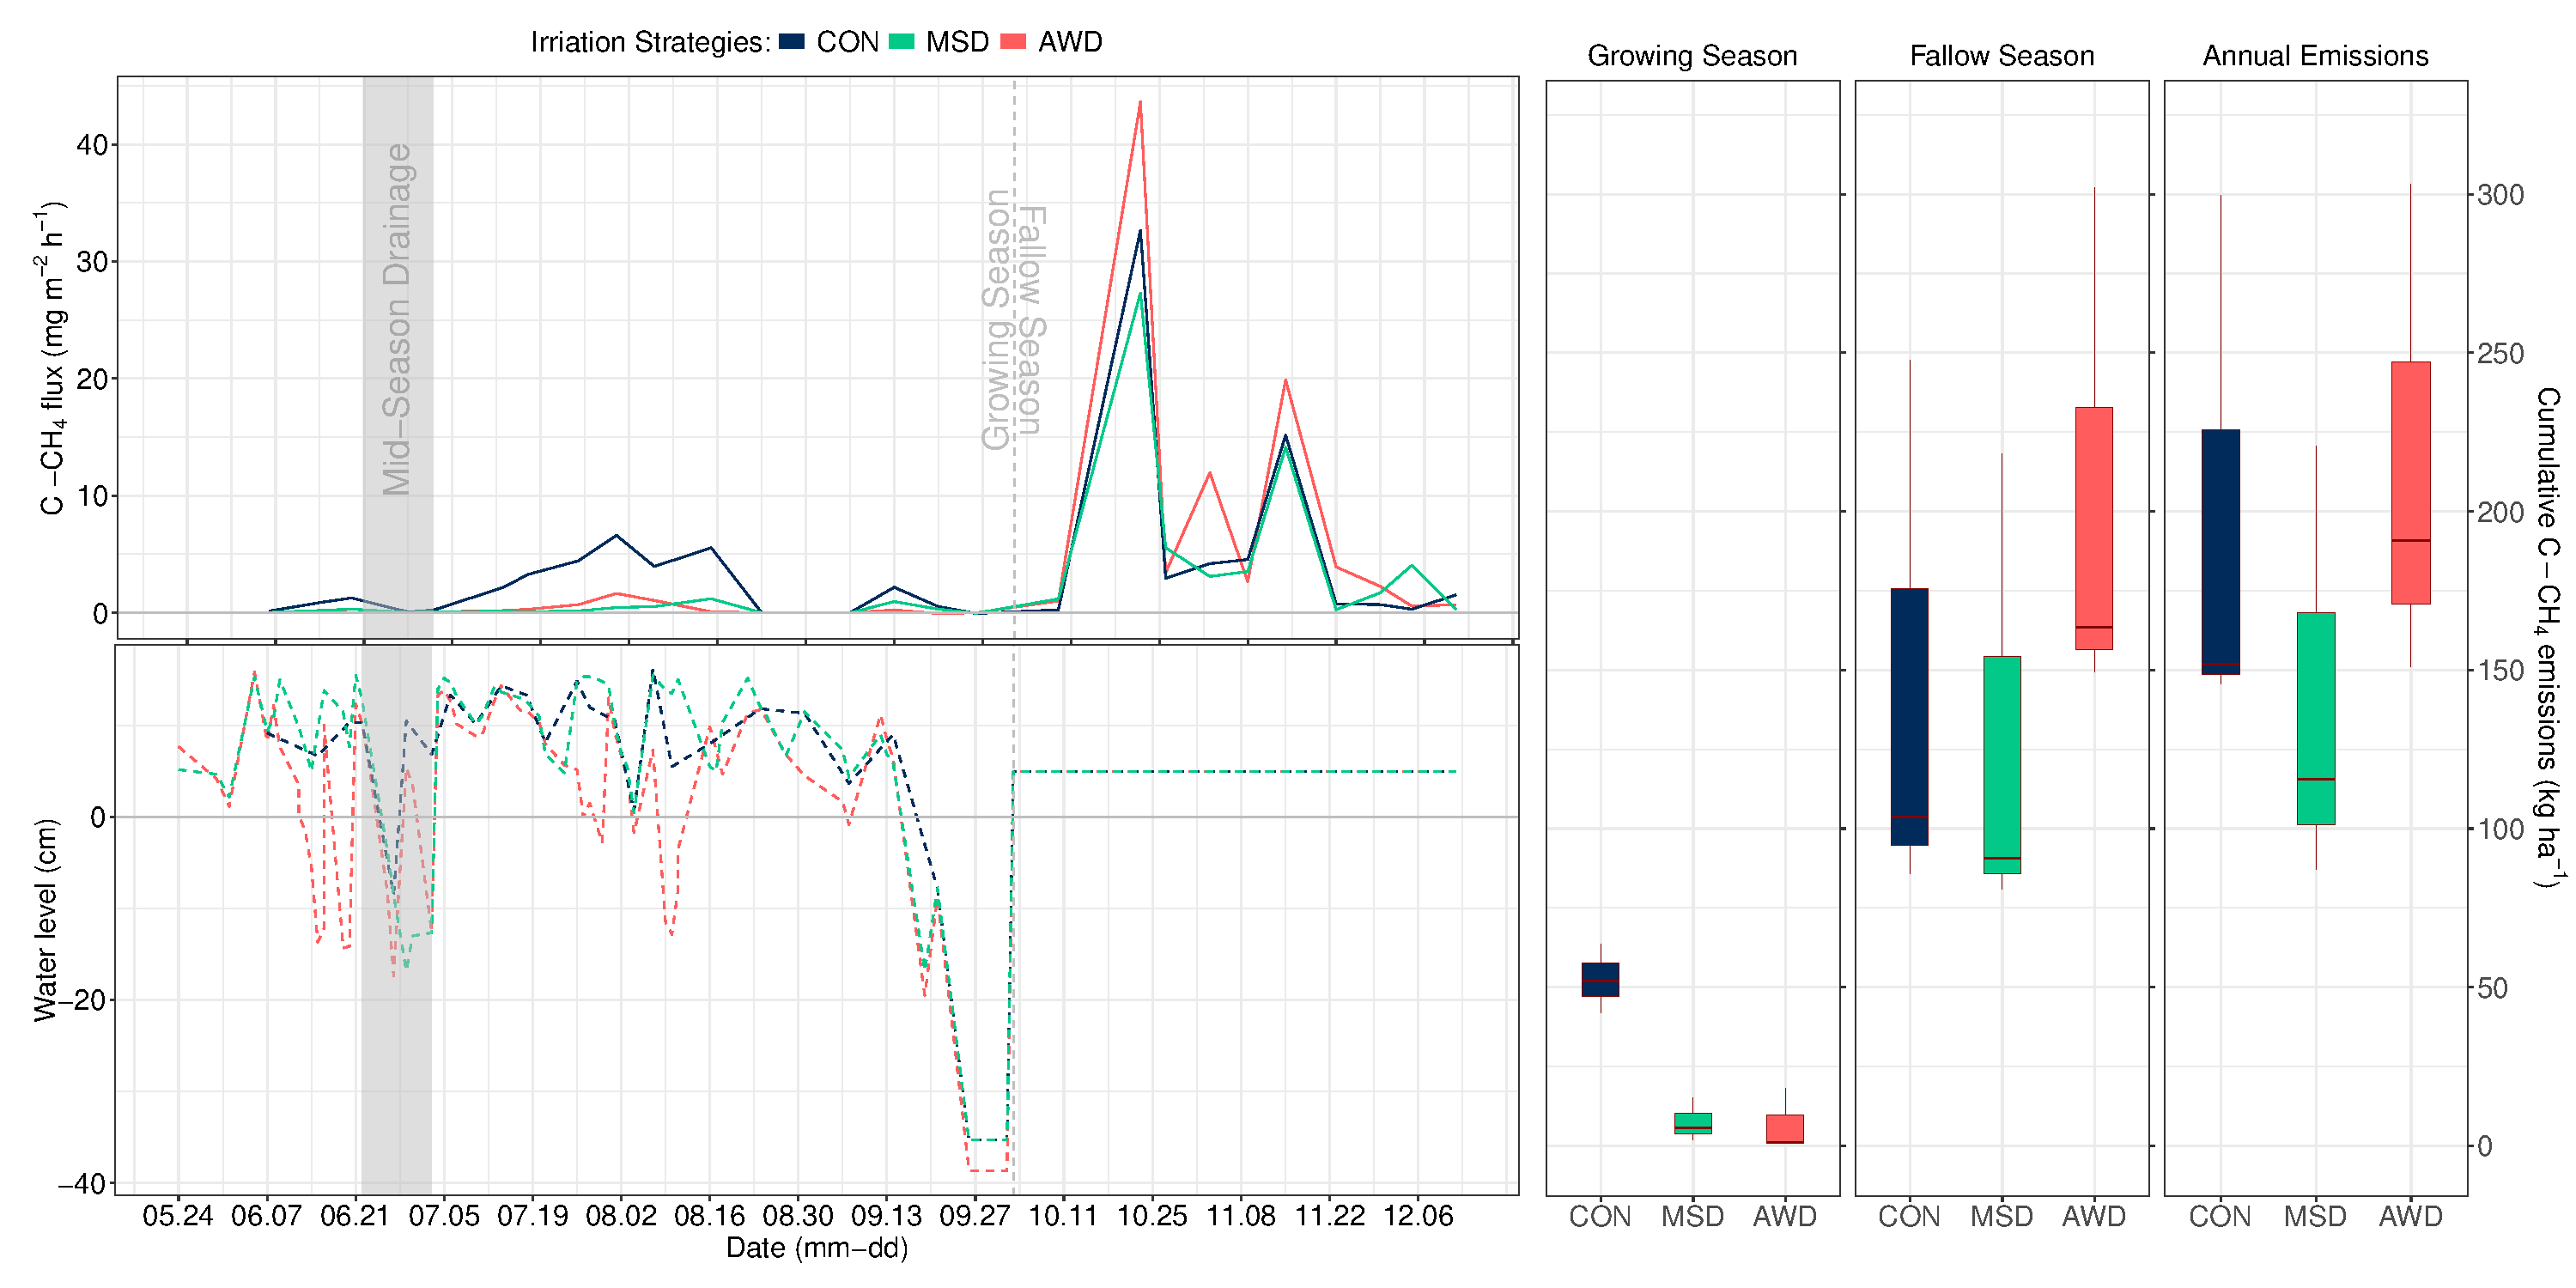
\includegraphics[scale=0.33, center]{Figures/Chapter_2/CH4_flux_water_acc.pdf}
	\captionof{figure}[CH4N2O]{Methane (CH$_{4}$, top-left panel) emission rates in mg m$^{-2}$ h$^{-1}$, and water level (bottom-left panel) in cm across the rice growing season for the three assessed irrigation strategies. Top-left panel lines are mean emissions per plot. Right boxplot panels show cumulative CH$_{4}$ emissions in kg ha$^{-1}$ for the rice growing season, fallow season and annual emissions.}  
	\label{CH4N2O}
\end{figure}
%\vspace{0.5cm}
%\end{landscape}

Fallow season emissions contributed an average of 87\% to overall annual cumulative CH$_{4}$ emissions, considering all assessed irrigation strategies, concentrated in three distinct sampled emission events rather than maintaining a constant seasonal pattern (Figures \ref{CH4N2O} and \ref{CH4_plot}). A significative interaction effect between season and irrigation treatments was identified ($\chi^2$=30.9, \textit{p}=$<$0.001). Emission patterns were inverted when transitioning from growing to fallow season. During the growing season, continuously flooded CH$_{4}$ fluxes were significantly higher than both AWD (\textit{z}=6.7, \textit{p}=$<$0.001) and MSD (\textit{z}=6.8, \textit{p}=$<$0.001) strategies. Fallow season emissions in AWD resulted higher than in continuous flooding (\textit{z}=1.9, \textit{p}=0.060) and MSD (\textit{z}=2.2, \textit{p}=0.031); no differences were registered in between continuously flooded and MSD plots (\textit{z}=0.2, \textit{p}=0.813). Model covariates such as water level ($\chi^2$=7.5, \textit{p}=0.006), soil temperature ($\chi^2$=21.3, \textit{p}=$<$0.001), atmospheric temperature ($\chi^2$=22.2, \textit{p}=$<$0.001) and soil electrical conductivity ($\chi^2$=11.3, \textit{p}=$<$0.001), as well as sampling date ($\chi^2$=12.4, \textit{p}=$<$0.001) as a model factor, resulted in significant effects on CH$_{4}$ emission rates. N$_{2}$O fluxes peaked in AWD plots during drainage periods, but also some emissions registered in plots under anoxic conditions (Figure \ref{N2O}). During the growing season, CH$_{4}$ emissions in continuously flooded plots averaged 52.5$\pm$6.2 kg ha$^{-1}$, while both non-continuous flooding strategies decreased these in approximately 86\%, with 6.8$\pm$5.7 and 7.6$\pm$3.9 kg ha$^{-1}$ emitted on average in MSD and AWD, respectively. The irrigation strategy with highest fallow season CH$_{4}$ emissions was AWD (205.1$\pm$48.7 kg ha$^{-1}$), followed by continuous flooding (145.7$\pm$51.2 kg ha$^{-1}$) and MSD (129.9$\pm$44.2 kg ha$^{-1}$). Considering overall annual cumulative CH$_{4}$ emissions, AWD (214.9$\pm$45.5 kg ha$^{-1}$) represented an 8\% increase in regards to continuously flooded (198.9$\pm$50.3 kg ha$^{-1}$) and 52\% to MSD (141.1$\pm$40.6 kg ha$^{-1}$) plots. 
\\ 

\begin{figure} [ht]
\captionsetup{justification=justified}
	\centering 
	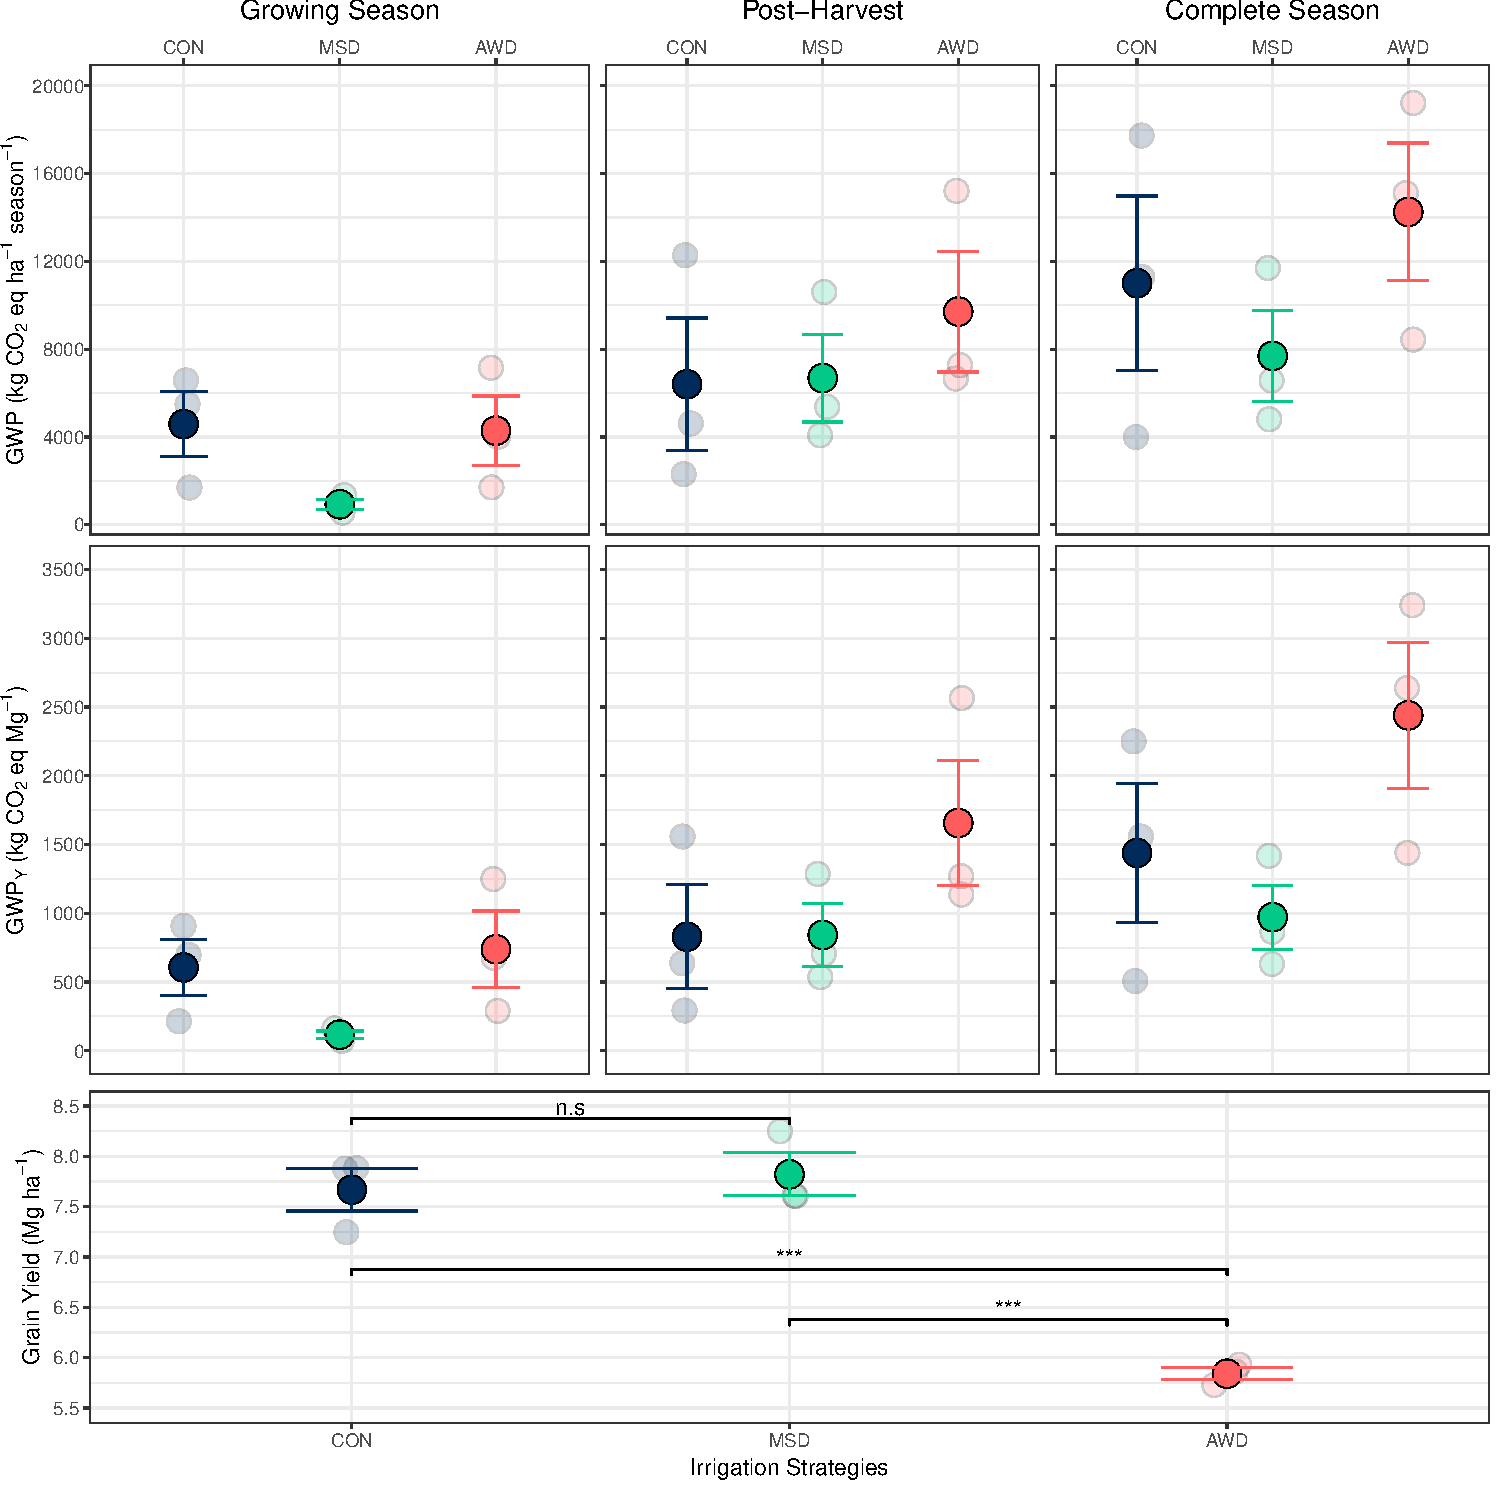
\includegraphics[scale=0.45, center]{Figures/Chapter_2/Yield_GWP_GWPY_arr.pdf}
	\captionof{figure}[GWPY]{Global warming potential (GWP, top plots), yield scaled global warming potential (GWPY, mid plots) and grain yield (bottom plot, in Mg ha$^{-1}$ at 14\% humidity) for the three assessed irrigation strategies. GWP and GWPY are calculated for the rice growing, fallow and complete (both growing and fallow) rice seasons. Solid dots show mean values, transparent dots show values per repetition. Error bars represent standard errors. Significance p-value ($\ast$ $\ast$ $\ast$ \textit{p}$<$0.001, $\ast$ $\ast$ \textit{p}$<$0.01; $\ast$ \textit{p}$<$0.05; n.s.: non significant) indicate statistical differences according to pairwise comparisons between the three assessed irrigation strategies and are only included in Grain Yield (bottom) panel, as no significative differences were found for GWP or GWPY.}  
	\label{GWPY}
\end{figure}
%\vspace{0.5cm}

Once cumulative CH$_{4}$ and N$_{2}$O emissions were accounted for, GWP was calculated and then yield scaled (GWPY) to compare water strategy effects on GHG emissions standardized to CO$_{2}$ equivalents (CO$_{2}$ eq) (Figure \ref{GWPY}). Compared to rice yields from continuously flooded plots (7.7$\pm$0.2 Mg ha$^{-1}$), MSD strategy maintained grain yield levels (7.8$\pm$0.2 Mg ha$^{-1}$) while AWD averaged a 24\% decrease (5.8$\pm$0.1 Mg ha$^{-1}$). This negative effect of AWD management caused an increase in warming potentials when scaling GWP to GWPY for these plots in comparison to other strategies. Overall annual warming potentials (GWP in Mg CO$_{2}$ eq ha$^{-1}$ and GWPY in Mg CO$_{2}$ eq Mg$^{-1}$), considering both growing and fallow seasons, were 11.5$\pm$3.9 and 1.5$\pm$0.5 for continuously flooded plots, 8.0$\pm$2.2 and 1.0$\pm$0.2 for MSD, and 14.6$\pm$3.2 and 2.5$\pm$0.5 for AWD. Even though no significant difference across treatments was identified for GWP ($\chi^2$=1.9, \textit{p}=0.393) or GWPY ($\chi^2$=3.8, \textit{p}=0.148), AWD represented average increases of 26.8\% and 66.2\% in GWP and GWPY, respectively, when compared to continuous flooding. \\ 

\subsection{Microbial biodiversity}

Structure of soil microbial communities varied through the assessed periods (Figure \ref{Beta}). Communities associated to plots managed under AWD strategy were significantly different to those in continuously flooded (growing season: \textit{F}=3.3, \textit{p}=0.001; fallow season: \textit{F}=1.7, \textit{p}=0.014) and in MSD ones (growing season: \textit{F}=2.0, \textit{p}=0.013; fallow season: \textit{F}=1.7, \textit{p}=0.009) through both periods. No significant differences were identified in between continuous flooding and MSD strategies (growing season: \textit{F}=1.5, \textit{p}=0.112; fallow season: \textit{F}=1.0, \textit{p}=0.398).\\

\begin{figure} [ht]
\captionsetup{justification=justified}
	\centering 
	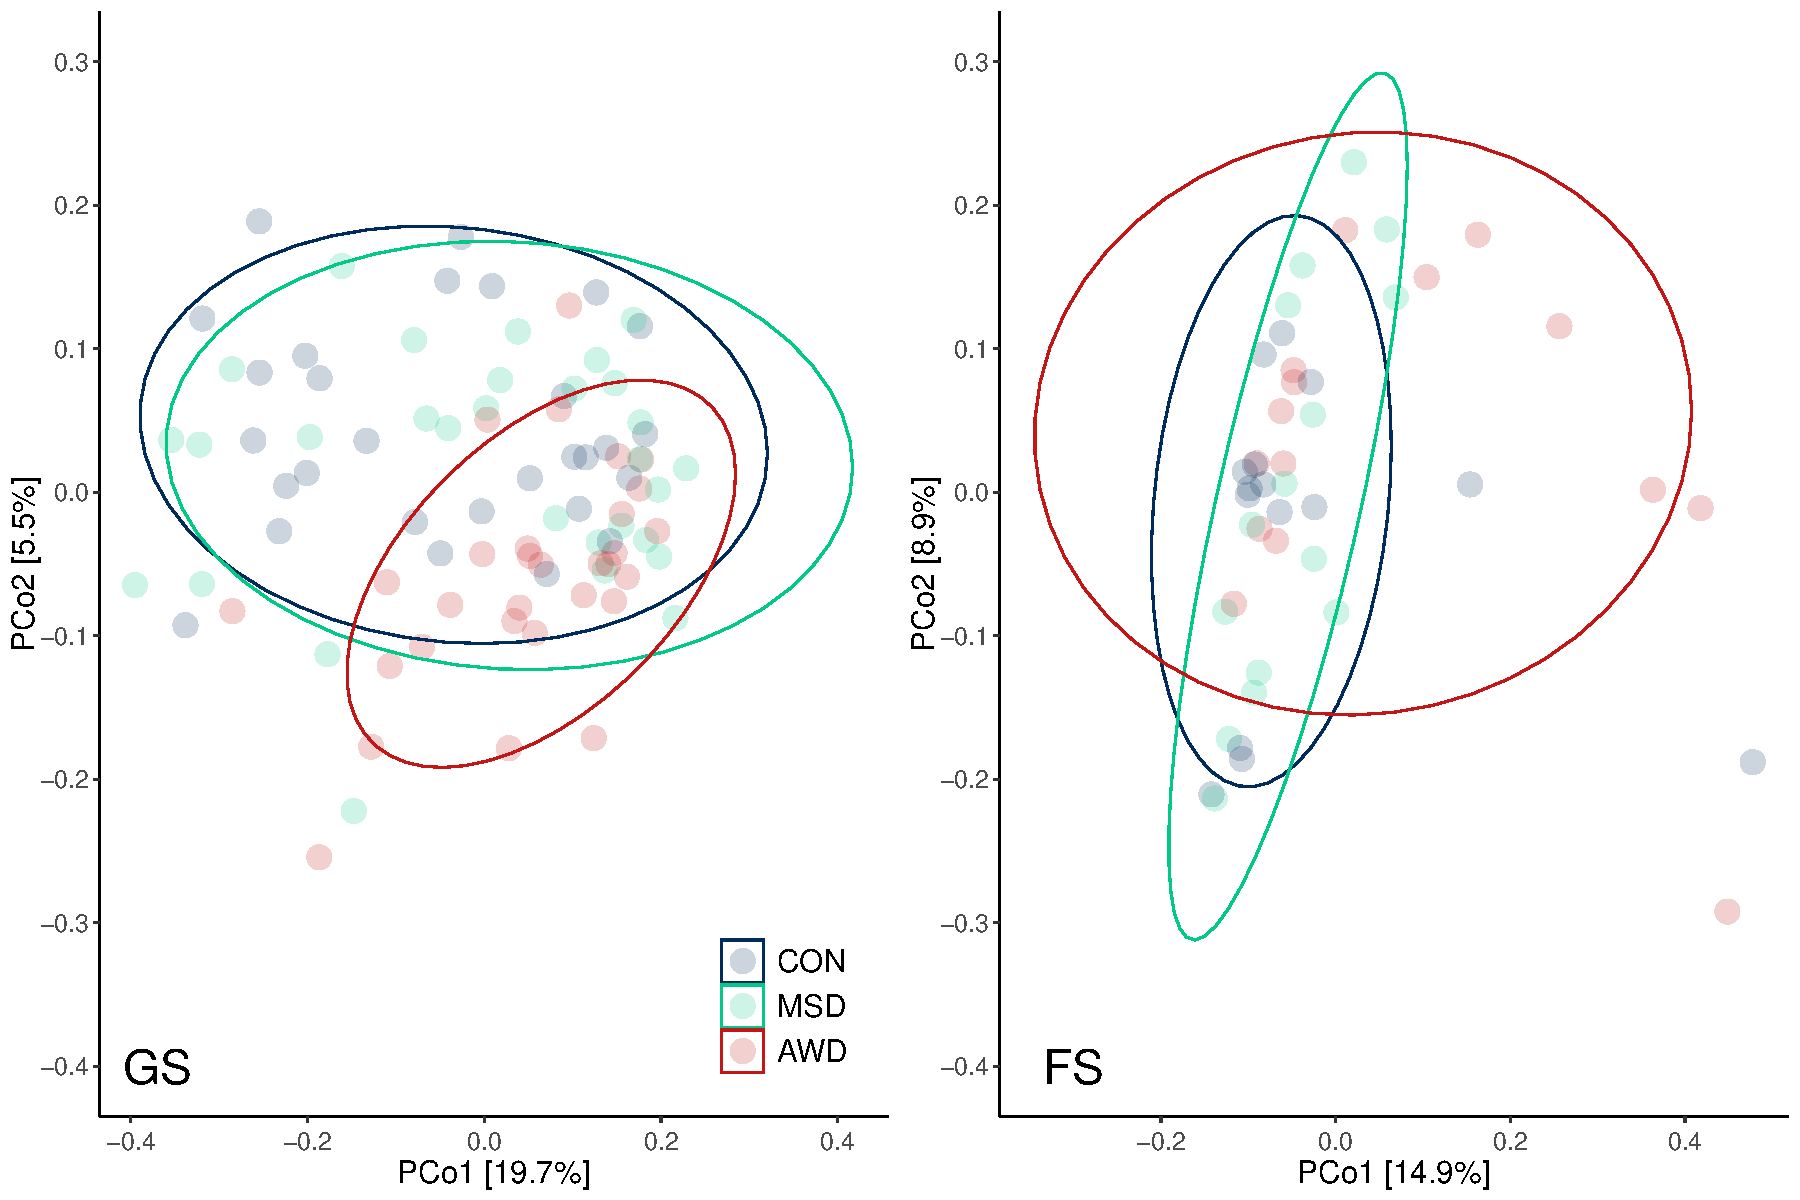
\includegraphics[scale=0.4, center]{Figures/Chapter_2/PCoA_stages_treatGSFS.pdf}
	\captionof{figure}[Beta]{Beta-diversity principal coordinate analysis (PCoA) derived from Bray–Curtis distances of soil microbial communities structure for both assessed periods (GS: Growing season; FS: Fallow season). Communities are clustered in regards to the irrigation strategies corresponding to the plot from which they were sampled.}  	
 \label{Beta}
\end{figure}
%\vspace{0.5cm}

No significant differences were identified among treatments in total bacterial ($\chi^2$=2.4, \textit{p}=0.294) and methanogenic archaeal ($\chi^2$=3.2, \textit{p}=0.205) abundances (Figure \ref{FuncGroups}a.-b.). Overall trends, nevertheless, showed lower total abundances for both groups of organisms in AWD plots when compared to both other irrigation strategies. When accounting for relative abundances among functional groups, populations of both methanogens (\textit{t}=2.9, \textit{p}=0.005) and methanotrophs (\textit{t}=2.3, \textit{p}=0.020) were more abundant in continuously flooded than those in AWD plots. Continuously flooded plots resulted also in higher relative abundance of methanogens than MSD plots (\textit{t}=3.6, \textit{p}=$<$0.001), no significant differences between these strategies was observed for methanotrophs (\textit{t}=1.0, \textit{p}=0.333). No differences in the abundance of alphaproteobacteria methanotrophs were found, whereas relative abundances for gammaproteobacteria methanotrophs within AWD plots resulted significantly lower than those in continuously flooded (\textit{t}=-2.4, \textit{p}=0.019) and MSD (\textit{t}=-2.5, \textit{p}=0.016). \\

\begin{figure} [ht]
\captionsetup{justification=justified}
	\centering 
	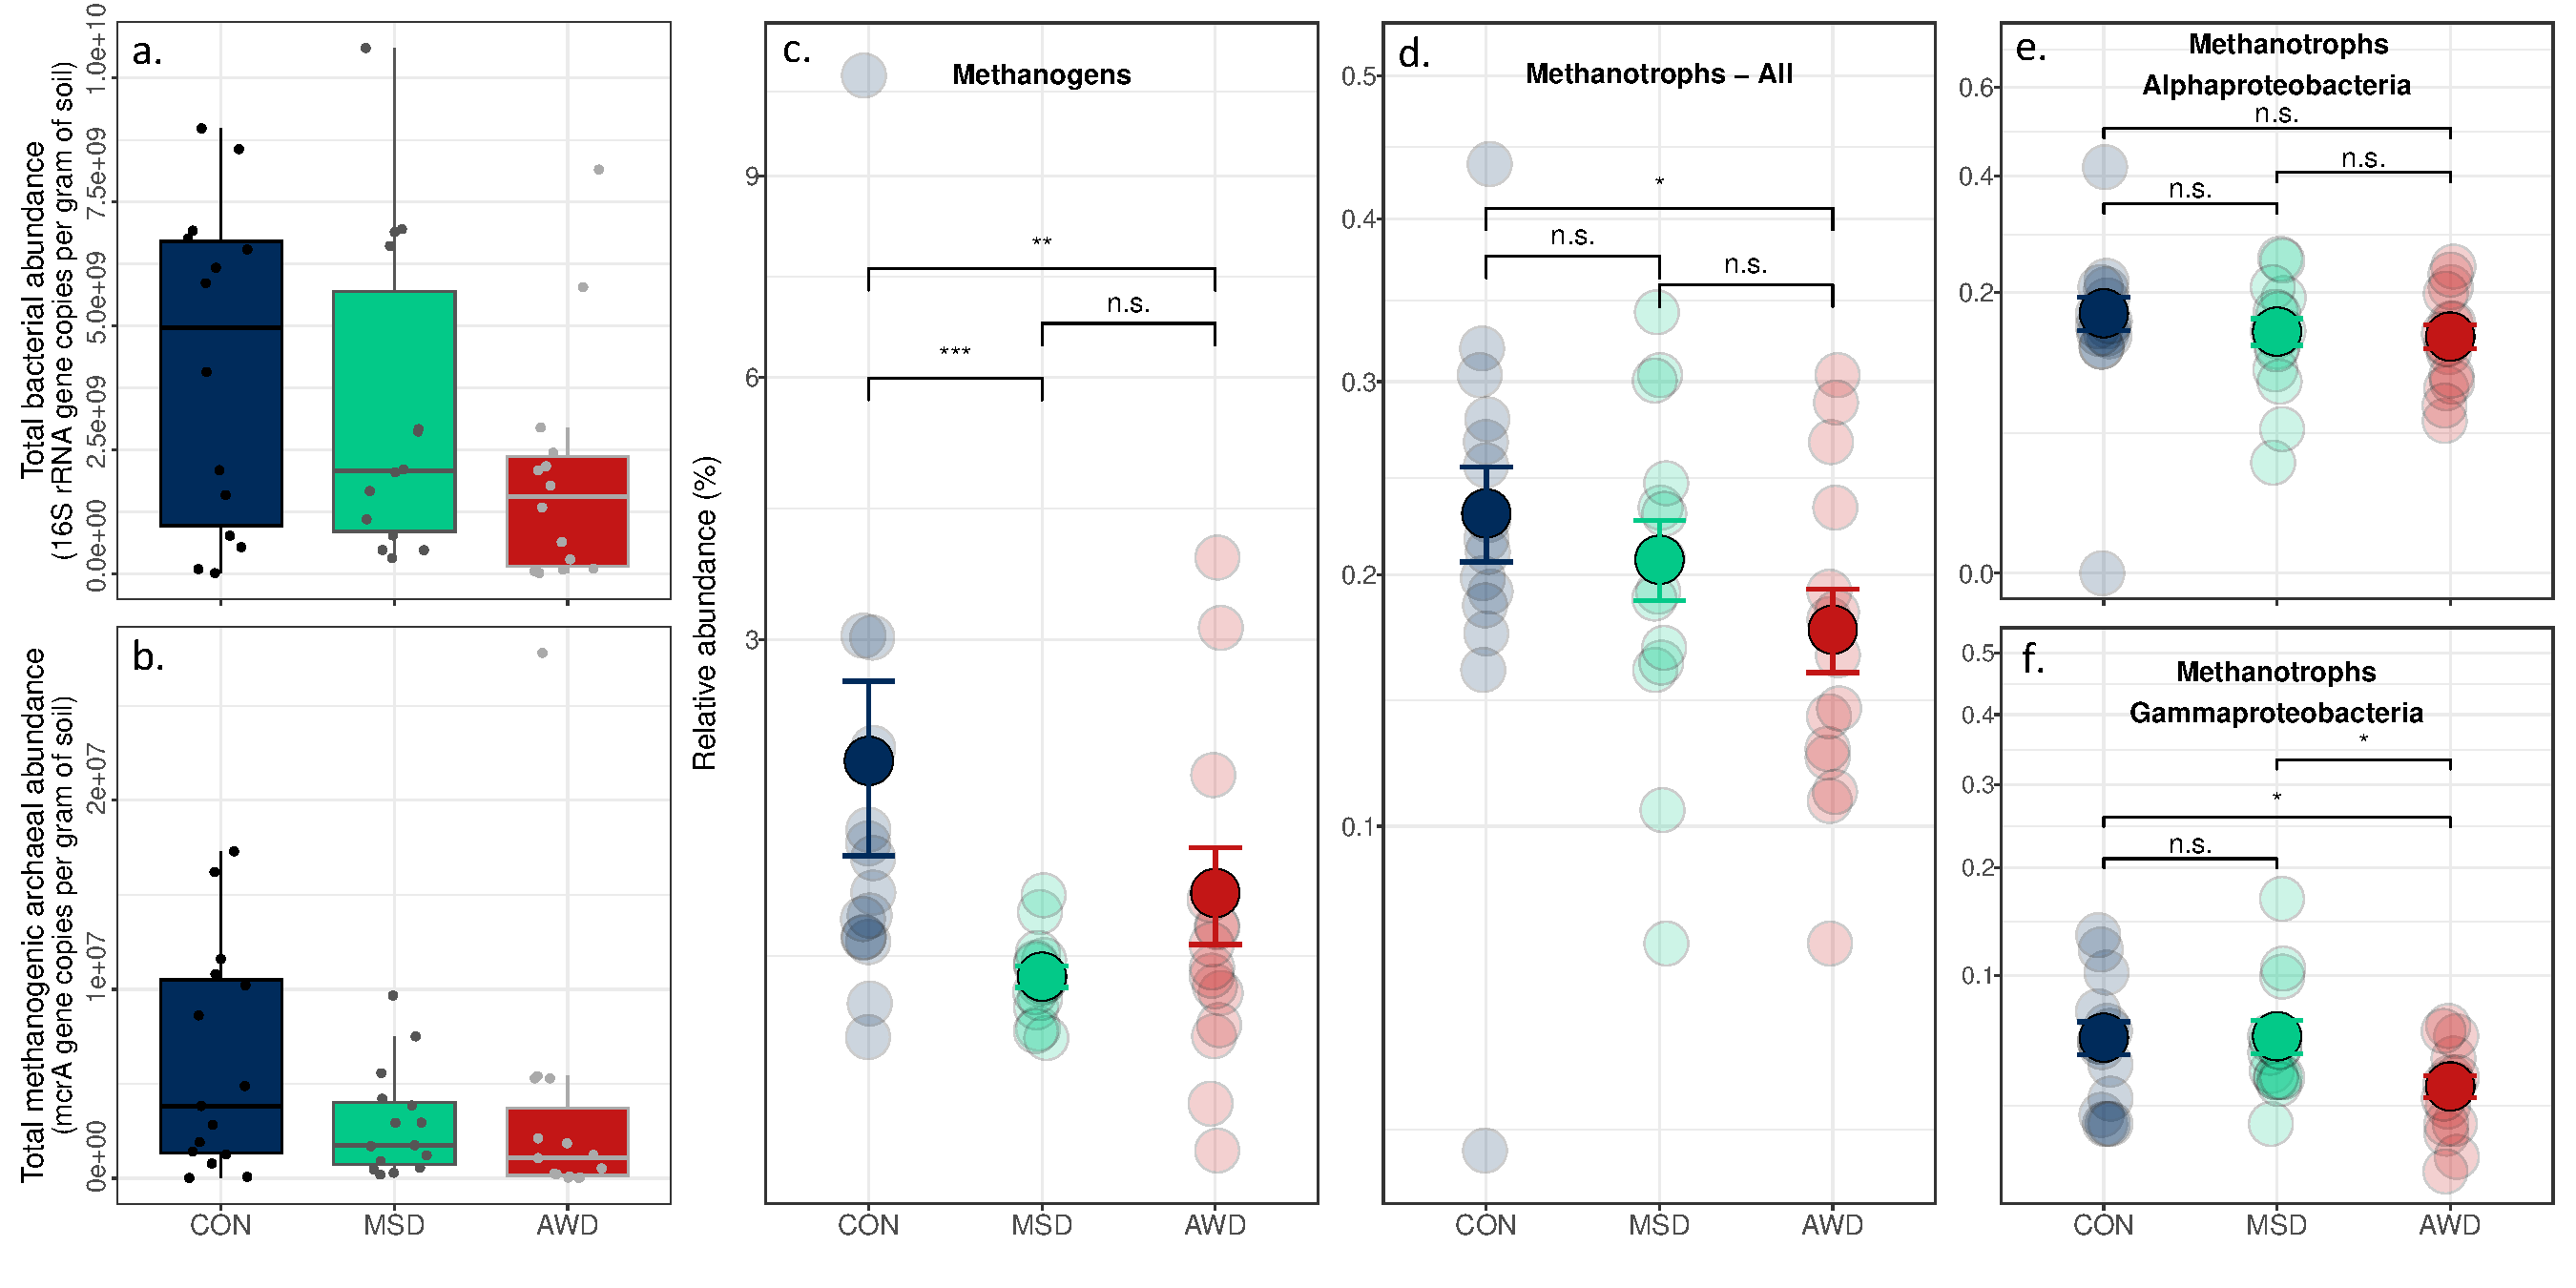
\includegraphics[scale=0.37, center]{Figures/Chapter_2/FuncGroups_plot_arr3_annot.pdf}
	\captionof{figure}[FuncGroups]{Fallow season total and relative abundances of soil microbial communities. Total bacterial (a.) and methanogenic archaeal (b.) abundances according to resulting copies per gram of soil for 16S rRNA and mcrA gene sequences, respectively. Bacterial and archaeal relative abundance (\%) according to their assigned functional groups (Methanogens (c.) and Methanotrophs - All (d.), Alphaproteobacteria (e.) and Gammaproteobacteria (f.)). Significance p-value ($\ast$ $\ast$ $\ast$ \textit{p}$<$0.001, $\ast$ $\ast$ \textit{p}$<$0.01; $\ast$ \textit{p}$<$0.05; n.s.: non significant) indicate statistical differences according to pairwise comparisons between the three assessed irrigation strategies for each functional group model.}  	\label{FuncGroups}
\end{figure}
%\vspace{0.5cm}

\section{Discussion}
\label{sec:discussion}

% Methane emissions 1: FS contribution to overall annual emissions 
Fallow season contribution to total annual cumulative CH$_{4}$ emissions (87\%) surpassed largely that of growing season emissions, as had been previously noted by \cite{martinez2018neglecting} for the Ebro Delta region. Averaged fallow season cumulative CH$_{4}$ emissions within mesocosm units set up from plots kept previously flooded during the growing season (145.7 kg ha$^{-1}$) were comparable to fallow season field measurements recorded at a larger scale for the whole Delta region (163.9 kg ha$^{-1}$, \cite{martinez-eixarch2021a}), peaking as well during October. Higher growing season CH$_{4}$ emissions registered for the region by \cite{martinez-eixarch2021a} (96.6 versus 52.5 kg ha$^{-1}$ recorded in this current study) might have been a product of the high soil clay content in our site, as a strong negative relation between this soil property and CH$_{4}$ emissions was identified in that previous study. Other temperate rice studies resulting in higher emissions in growing than in fallow seasons have either lacked straw incorporation \citep{reba2019} or have being conducted in regions with lower atmospheric temperatures during fallow seasons \citep{fitzgerald2000, adviento-borbe2013, lahue2016, peyron2016, wust-galley2023} (Figure \ref{temp}). Increased microbial activity due to higher fallow season soil temperatures \citep{conrad2023}, and the adaptation of soil microbial communities to such fallow season conditions through several years of rice production under the same edaphoclimatic conditions and agronomic practices \citep{jangid2011, lagomarsino2016a, conrad2020, hester2022}, are potential mechanisms explaining the contrasting CH$_{4}$ emissions pattern in between growing and fallow season in our study system in contrast to other temperate rice agroecosystems. \\ 

% Methane emissions 2: Mitigation during GS and legacy effects over FS
A positive effect of both non-continuous flooding strategies as climate change mitigation practices was observed through a steep decrease in growing season CH$_{4}$ emissions (86\%), when compared to continuously flooded plots. This decrease is higher than the average 53\% CH$_{4}$ emission decrease identified by \cite{jiang2019water} through a global meta-analysis, however, it is in line with that reported by studies in temperate rice systems \citep{linquist2015, lahue2016}. More noteworthy were the effects of these irrigation strategies when observing the following flooded fallow season, where CH$_{4}$ emission patterns changed from AWD being the strategy with lowest to the one with highest emissions. These differences in between CH$_{4}$ emissions during a flooded fallow season from plots previously managed under different irrigation strategies during the growing season suggest the presence of legacy effects of past soil moisture on CH$_{4}$ emissions. \cite{lahue2016} had previously concluded that AWD effects did not extend into fallow seasons under similar management (straw incorporated and flooded fallow season), nevertheless, as discussed above, lower temperatures during fallow seasons might have decreased CH$_{4}$ emissions during that period, hindering potential effects in comparison to our current results. The highest fallow season CH$_{4}$ emissions corresponded to AWD, contradicting the initially hypothesized extended climate change mitigation effect of this strategy over the fallow season. Nonetheless, growing season MSD did manage to maintain lower fallow season CH$_{4}$ emissions when compared to both other strategies. This MSD mitigation effect decreasing CH$_{4}$ emissions through both rice seasons results of great interest as it requires as well significantly less planning and field effort than that of an AWD strategy.\\ 

% Methane emissions 3: cum.CH4, GWP, GWPY, Yield
Although implementing an AWD strategy decreases cumulative CH$_{4}$ emissions during the growing season, when considering its fallow season emission peaks the overall annual effect is negative as cumulative CH$_{4}$ emissions, GWP and GWPY are higher than those registered for both other assessed strategies (Figures \ref{CH4N2O} and \ref{GWPY}). The effects on yields were variable in between non-continuous flooding irrigation strategies as, even though MSD proved to maintain production levels similar to those in continuously flooded plots, a strong decline in grain yield (24\%) was observed for AWD. The main drivers of such decline are the length of drying periods, ground water-table depth and evaporative demand \citep{tuong2003rice}. A significant AWD yield decline of 19\% was previously registered in the same study site by \cite{martinez-eixarch2021}, which identified panicle density and grain number per panicle as the most affected yield components. \cite{monaco2021} found as well that grain number per panicle had significative declines under AWD in comparison to continuous flooding in a similar system. Larger yield reduction in our current study might be explained by a second period of drain-flood cycles during grain ripening, which was not implemented in that previous experience. For the particular agroecosystem assessed in this study, MSD represented a potentially more effective strategy, achieving the lowest cumulative CH$_{4}$ emissions, GWP and GWPY across seasons without grain yield decreases. In contrast to the observed effects on CH$_{4}$ fluxes across both seasons, a lower number of observations (three per irrigation strategy) might have impeded the identification of significant effects of irrigation strategies on cumulative CH$_{4}$ emissions. Further research on these effects is recommended to fully understand the overall impacts of these practices on global change, specifically for rice producing regions with high CH$_{4}$ emissions during fallow seasons.\\ 

% Microbial biodiversity 1: Emission-microbiology transition
The hypothesis of a long-lasting mitigation effect of AWD implemented during the growing season on fallow season CH$_{4}$ emissions derived from the notions of: (i) a decreased grain yield in AWD plots during the previous 2022 season, which was expected to be the case again for the current season, resulting in less biomass produced and less straw incorporated (lower carbon inputs); and (ii) of microbial communities adapting progressively to irrigation practices, reinforcing their effect on GHG emissions over time, as proposed by \cite{lagomarsino2016a}. The rejection of this initial hypothesis required revisiting these assumptions. Lower labile soil organic carbon due to past paddy management, such as lower carbon inputs as a consequence of lower amounts of straw incorporated, can result in decreased CH$_{4}$ emissions \citep{hatala2012}. Nevertheless, even though the prediction of reduced grain yields was met, AWD management did not present lower straw incorporation (Table \ref{straw}). Effects of non-continuous flooding practices over belowground biomass have so far been inconclusive in the literature, as negative \citep{oliver2019} and insignificant \citep{carrijo2018} effects have been reported. No particular differences were observed for root development in between plots in this current study (Table \ref{straw}). No evident differences in carbon input among strategies as an explanatory variable for the registered results suggests that these effects might rather be explained by changes in soil microbial community structure and composition. \\

% Microbial biodiversity 2: Beta diversity and relative abundance
Microbial communities differed among irrigation strategies during the growing season, with AWD showing a particularly different structure than the other strategies (Figure \ref{Beta}). During the subsequent flooded fallow season, microbial communities did not converge into similar structures despite a cease in disturbances (draining events) and plots being subjected to the same flooding conditions. This preserved microbial community divergence across the treatments beyond the implementation of the disturbance reinforces the idea of irrigation strategies legacy effects on CH$_{4}$ emissions. Past soil moisture content effect on microbial community composition and activity has to be considered as an important driver of microbiological processes in soils undergoing flooding and drainage cycles, as previous dry periods are associated with decreased microbial richness and more even communities \citep{banerjee2016}. Structure variation in between irrigation strategies and rice seasons is driven by soil bacterial and archaeal abundance dependency on soil oxic-anoxic conditions, being higher in flooded fields \citep{breidenbach2014}. Accordingly, our results showed lower abundance of methanogenic archaea and methanotrophic bacteria in AWD \citep{hester2022} (Figure \ref{FuncGroups}c.-d.). Legacy effects of drought periods on soil microbial community composition have been also reported in grassland systems \citep{vilonen2023}.\\

% Microbial biodiversity 3: New hypothesis
Soil CH$_{4}$ concentration is one of the controlling factors for methanotrophic growth \citep{jiao2006}. We hypothesize that a high soil CH$_{4}$ availability due to higher methanogenic activity during the growing season might have driven an enrichment of methanotrophic populations under continuous flooding conditions. Intermittent soil aeration in AWD, on the contrary, depleted soil CH$_{4}$ availability during the growing season due to its negative effect on methanogen abundance, leading as well to a decrease in methanotrophic bacteria populations. The relative abundance of gammaproteobacteria was particularly affected by AWD when compared to both other irrigation strategies (Figure \ref{FuncGroups}f.). In contrast to alphaproteobacteria (Figure \ref{FuncGroups}e.), these methanotrophs are able to oxidize CH$_{4}$ also under flooded anoxic conditions \citep{schorn2024}, therefore, a decrease in their abundance within the AWD microbial community can lead to lower methanotrophic activity when moving towards a flooded fallow season. Straw incorporation at the beginning of the fallow season results in large inputs of readily available organic matter and, consecutively, on an increase in CH$_{4}$ production rates by methanogenic archaeal populations \citep{wassmann1993methane}. Since the difference between CH$_{4}$ production and consumption determines resulting emissions \citep{conrad2009global}, a higher consumption by well established methanotrophic bacteria populations in continuously flooded plots may have kept fallow season CH$_{4}$ emissions at lower rates than those in plots where AWD had been implemented. As a result of this, CH$_{4}$ mitigation during the growing season in AWD was eventually offset by the increased fallow CH$_{4}$ emissions. Differences among outcomes from both non-continuous flooding strategies can also be understood through the analysis of their effects on microbial communities. Whereas a unique drainage might have decreased the relative abundance of methanogens surviving into the fallow season when comparing to continuously flooded plots, methanotrophs were apparently more resilient to this single disturbance, as their abundance was unaffected. This contrasting response to drainage periods between methanogens and methanotrophs suggests a divergent ability to recover after drainage events. Alterations in biogeochemical properties of paddy soil driven by changes in soil redox could have also played a role in this differing response. For instance, nutrient cycling (i.e., N and Fe) is modified with alternated reduced and oxic conditions in soils, with further implications in microbial activity \citep{chen2023}. \\

% Microbial biodiversity 4: Activity hypothesis and reach of the study
The current analysis focused on the abundance rather than on the activity of organisms present within soil microbial communities during one rice fallow season. 
Besides growing season soil CH$_{4}$ availability as a driver of fallow season microbial abundances and CH$_{4}$ production and emission, potential change in microbial activity could also be a mechanism involved in these processes.
\cite{breidenbach2014} described how draining fields leads to lower abundances of bacteria and archaea, but also to higher microbial activity (in terms of increased cellular levels of rRNA) as a possible mechanism of stress response of surviving anaerobic microorganisms to be prepared for re-flooding. Methanogenic archaea in AWD plots, even if decreased in numbers compared to continuous flooding ones (Figure \ref{FuncGroups}c.), might have been better prepared to resume their activity once anoxic conditions and carbon input were provided. A steeper depletion of methanogen populations caused by a single and longer drainage in MSD plots could have potentially made this defense mechanism undetectable in comparison to carbon metabolism pathways more prevalent in the overall community, driving the observed fall in CH$_{4}$ emissions for this strategy. Methanotrophs, however, did not seem to follow this same response mechanism as no emission mitigation effect was observed in AWD plots. Drainage and wetting cycles can reduce methane oxidation potential in rice paddy fields \citep{ma2013}. Furthermore, methanotrophic bacteria did not show a strong susceptibility to longer MSD drainage but responded in accordance to the gradient of disturbance in terms of frequency of drainage events. Additionally to growing season soil CH$_{4}$ availability, abundance of methanotrophic microorganisms could be determined as well by the recovery time after each disturbance event, as microbial communities in disturbed soils tend to return to previous stability states with time \citep{jangid2011}. A single disturbance and sufficient time for methanotroph communities to stabilize after it in MSD might explain the observed intermediate effect of this strategy on relative abundance levels. Lower relative abundance of methanogens and populations of methanotrophs large enough to consume their CH$_{4}$ production could explain the positive mitigation effects observed in MSD in terms of cumulative CH$_{4}$, GWP and GWPY. \\

% Discussion closure: Agricultural mgmt and mitigation practice recommendations, and short-term experiment comment
The severe drought conditions under which this experiment was conducted highlight the double role that irrigation strategies might play in rice paddies. Besides their potential mitigation effects due to reduced GHG emissions, they serve as well as climate change adaptation practices allowing farmers to maintain production reducing water use \citep{ye2013}. Our results suggest that a single drain is a more efficient irrigation management addressing GHG emissions in our assessed system, compared to both continuous flooding and AWD. Therefore, considering AWD as a one-size-fits-all solution is not recommended and its scale up should follow proper assessment under local conditions. Specific environmental and agronomic conditions (e.g. high fallow season temperatures) might turn this practice into a detrimental strategy when considering overall annual effects. Even though our study considered the cumulative effect of two years of irrigation strategies, GHG emissions and effects on soil microbial communities correspond to those registered during one growing and its subsequent fallow season, thus representing short-term effects. Further studies considering not only microbial abundance but also their activity through longer time-scale field studies are necessary to determine the exact mechanisms responsible for different effects of irrigation strategies on the presence and prevailing metabolic pathways of specific functional groups of soil microorganisms, and the consequent effects on CH$_{4}$ emissions across rice production seasons.\\ 

\section{Conclusions}
\label{sec:conc}

Under the particular edaphoclimatic conditions and agricultural practices carried out in the Ebro Delta rice agroecosystems, 
% removed after Reviewer #4's suggestions: CH$_{4}$ fluxes peak during the fallow season, dwarfing those observed across the crop growing season. 
a single drainage event, as in MSD irrigation, proved effective as a mitigation strategy considering an overall annual period. Even though AWD is an effective climate change mitigation practice during the growing season, its effects during the fallow season are less clear. Higher CH$_{4}$ emissions during the fallow season suggest potential negative effects of AWD management compared to continuous flooding in terms of overall cumulative CH$_{4}$ emissions, GWP and GWPY. % removed after Reviewer #4's suggestions: Changes in the structure of soil microbial communities can be assessed as an approach to understand the effects of irrigation strategies on CH$_{4}$ emissions across seasons. AWD not only reduced methanogenic archaea, but also methanotrophic bacteria, ultimately leading to an increase in CH$_{4}$ emissions in comparison to continuous flooding. 
The persistence of microbial community structures with reduced abundances of methanogenic archaea and methanotrophic bacteria into the following flooded fallow season can hinder the expected mitigation effect of AWD. Our study suggests a legacy effect of irrigation strategies on soil community structure with implications on the dynamics of GHG emissions in the subsequent season following their implementation. Lower relative abundance of methanogenic archaea and higher presence of methanotrophic organisms under a MSD management might explain its positive potential as a climate change mitigation practice. Implementing an AWD irrigation strategy should not be considered as a one-size-fit-all solution for climate change mitigation in rice agroecosystems. The effects of climate change mitigation practices should be assessed beyond the season in which they are implemented since they may cause persistent effects on GHG emission drivers, such as the composition of soil microbial communities, increasing their potential capacity to alter GHG dynamics.\\

\section*{ACKNOWLEDGEMENTS}
\label{sec:ackn}

This study was funded by the Spanish Ministry of Economy, Trade and Enterprise (MINECO) through the Grant PID2020-118650RR-C31 (funded by MCIN/ AEI/ 10.13039/ 501100011033). The Government of Catalonia funded the predoctoral fellwoship of S.E.-P. through the projects AgriCarboniCat and AgriRegenCat. N.P.-M. is supported by a Spanish ‘Ramón y Cajal’ fellowship (RYC-2021-033599-I). We thank Joan Noguerol for all his support in gas chromotagraphy analysis and Prof. Bruce A. Linquist for his reviews and constructive feedback. We also thank Andrea Bertomeu, Vicent Cebolla, Joan Didac Bertomeu, Raul Llevat, Guillem Rovira and Juan Blas Fernández-Araujo for all their field support. The support of the CERCA Programme, Generalitat de Catalunya, is also acknowledged.

\subsection*{Competing interests statement}
\label{sec:interests}

The authors declare that they have no known competing financial interests or personal relationships that could have appeared to influence the work reported in this paper.

%\pagebreak
 
%\bibliography{cas-refs}

\pagebreak

%\appendix
%\section*{Appendices}
%\label{sec:ann}
%
%\setcounter{figure}{0}
%\renewcommand{\thefigure}{A.\arabic{figure}}

\newcommand{\appendixBtables}{
  \renewcommand{\thetable}{B.\arabic{table}}
  \setcounter{table}{0}
}

\section{Appendix to Chapter 2}
\addcontentsline{toc}{chapter}{Appendix to Chapter 2}
\renewcommand{\thefigure}{B.\arabic{figure}}
\setcounter{figure}{0}
%\renewcommand{\thetable}{B.\arabic{table}}
%\setcounter{table}{0}

\appendixBtables  % ← Ensures tables start with B.1, B.2, etc.

% CH4 Flux with empiric fluxes per plot:

\begin{figure*}[htbp]
\captionsetup{justification=justified}
	\centering 
	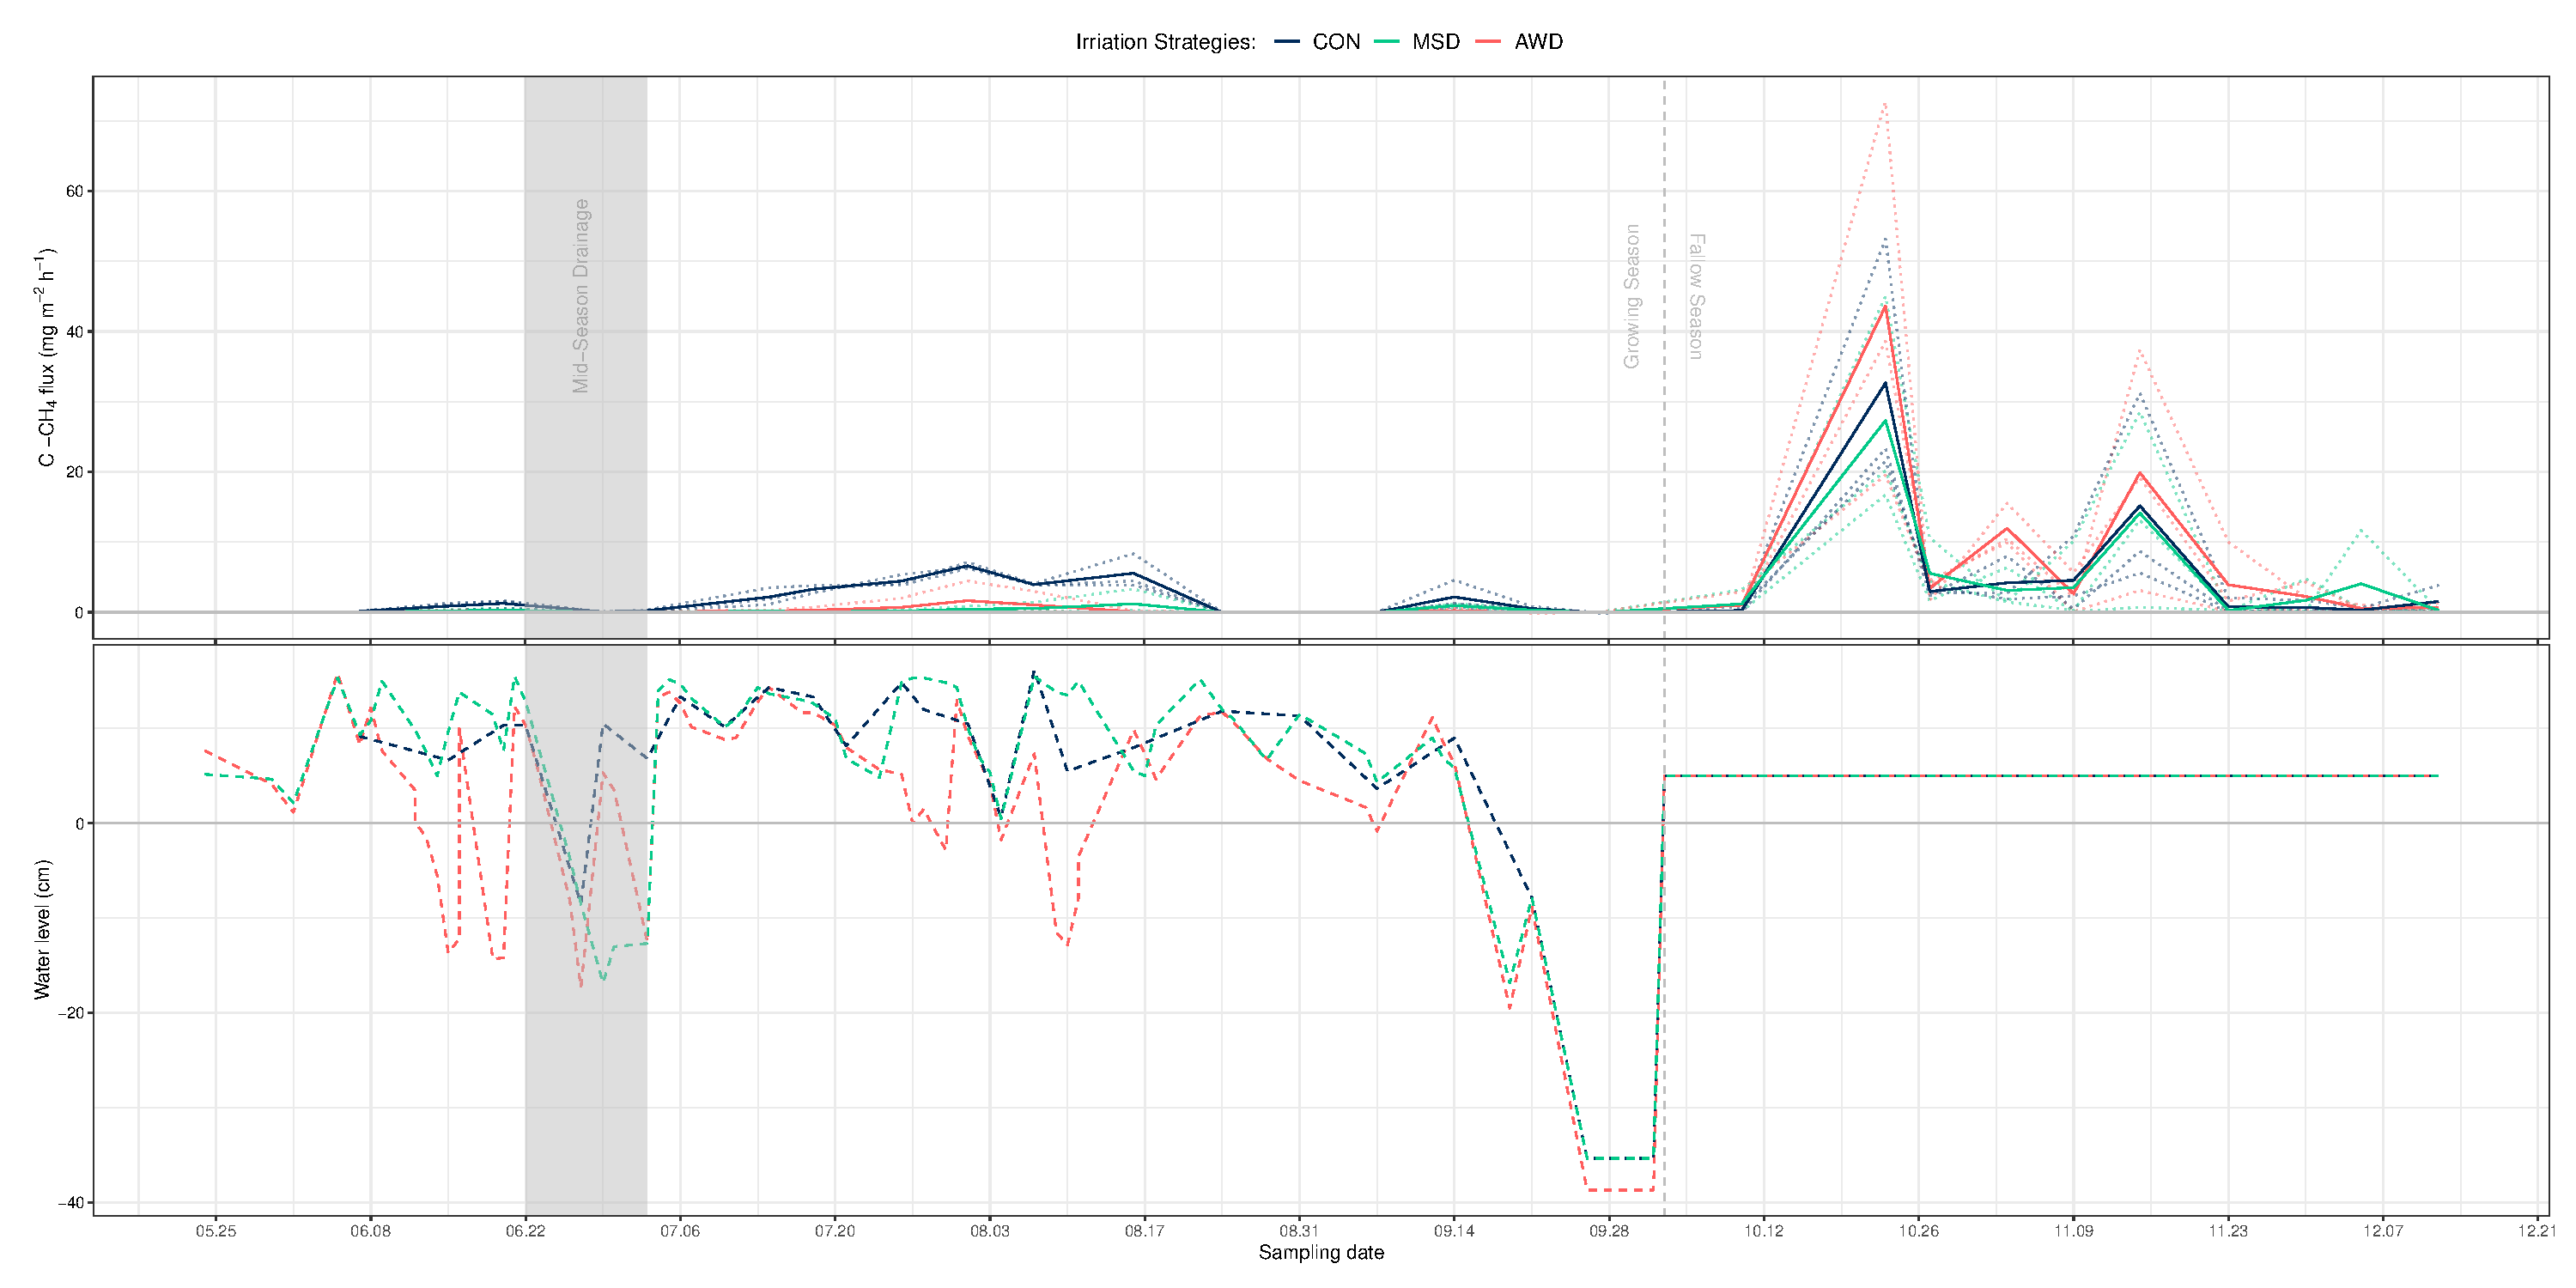
\includegraphics[scale=0.35, center]{Figures/Chapter_2/CH4_flux_water.pdf}
	\captionof{figure}[Treats]{Methane (CH$_{4}$, top panel) emission rates in mg m$^{-2}$ h$^{-1}$, and water level (bottom panel) in cm across the rice growing and fallow seasons for the three assessed irrigation strategies. Discontinuous lines in the top panel are mean emissions per plot, continuous lines are treatment means.}     \label{CH4_plot}
\end{figure*}
%\vspace{0.5cm}\\

% N2O Flux:

\begin{figure*}[htbp]
\captionsetup{justification=justified}
	\centering 
    	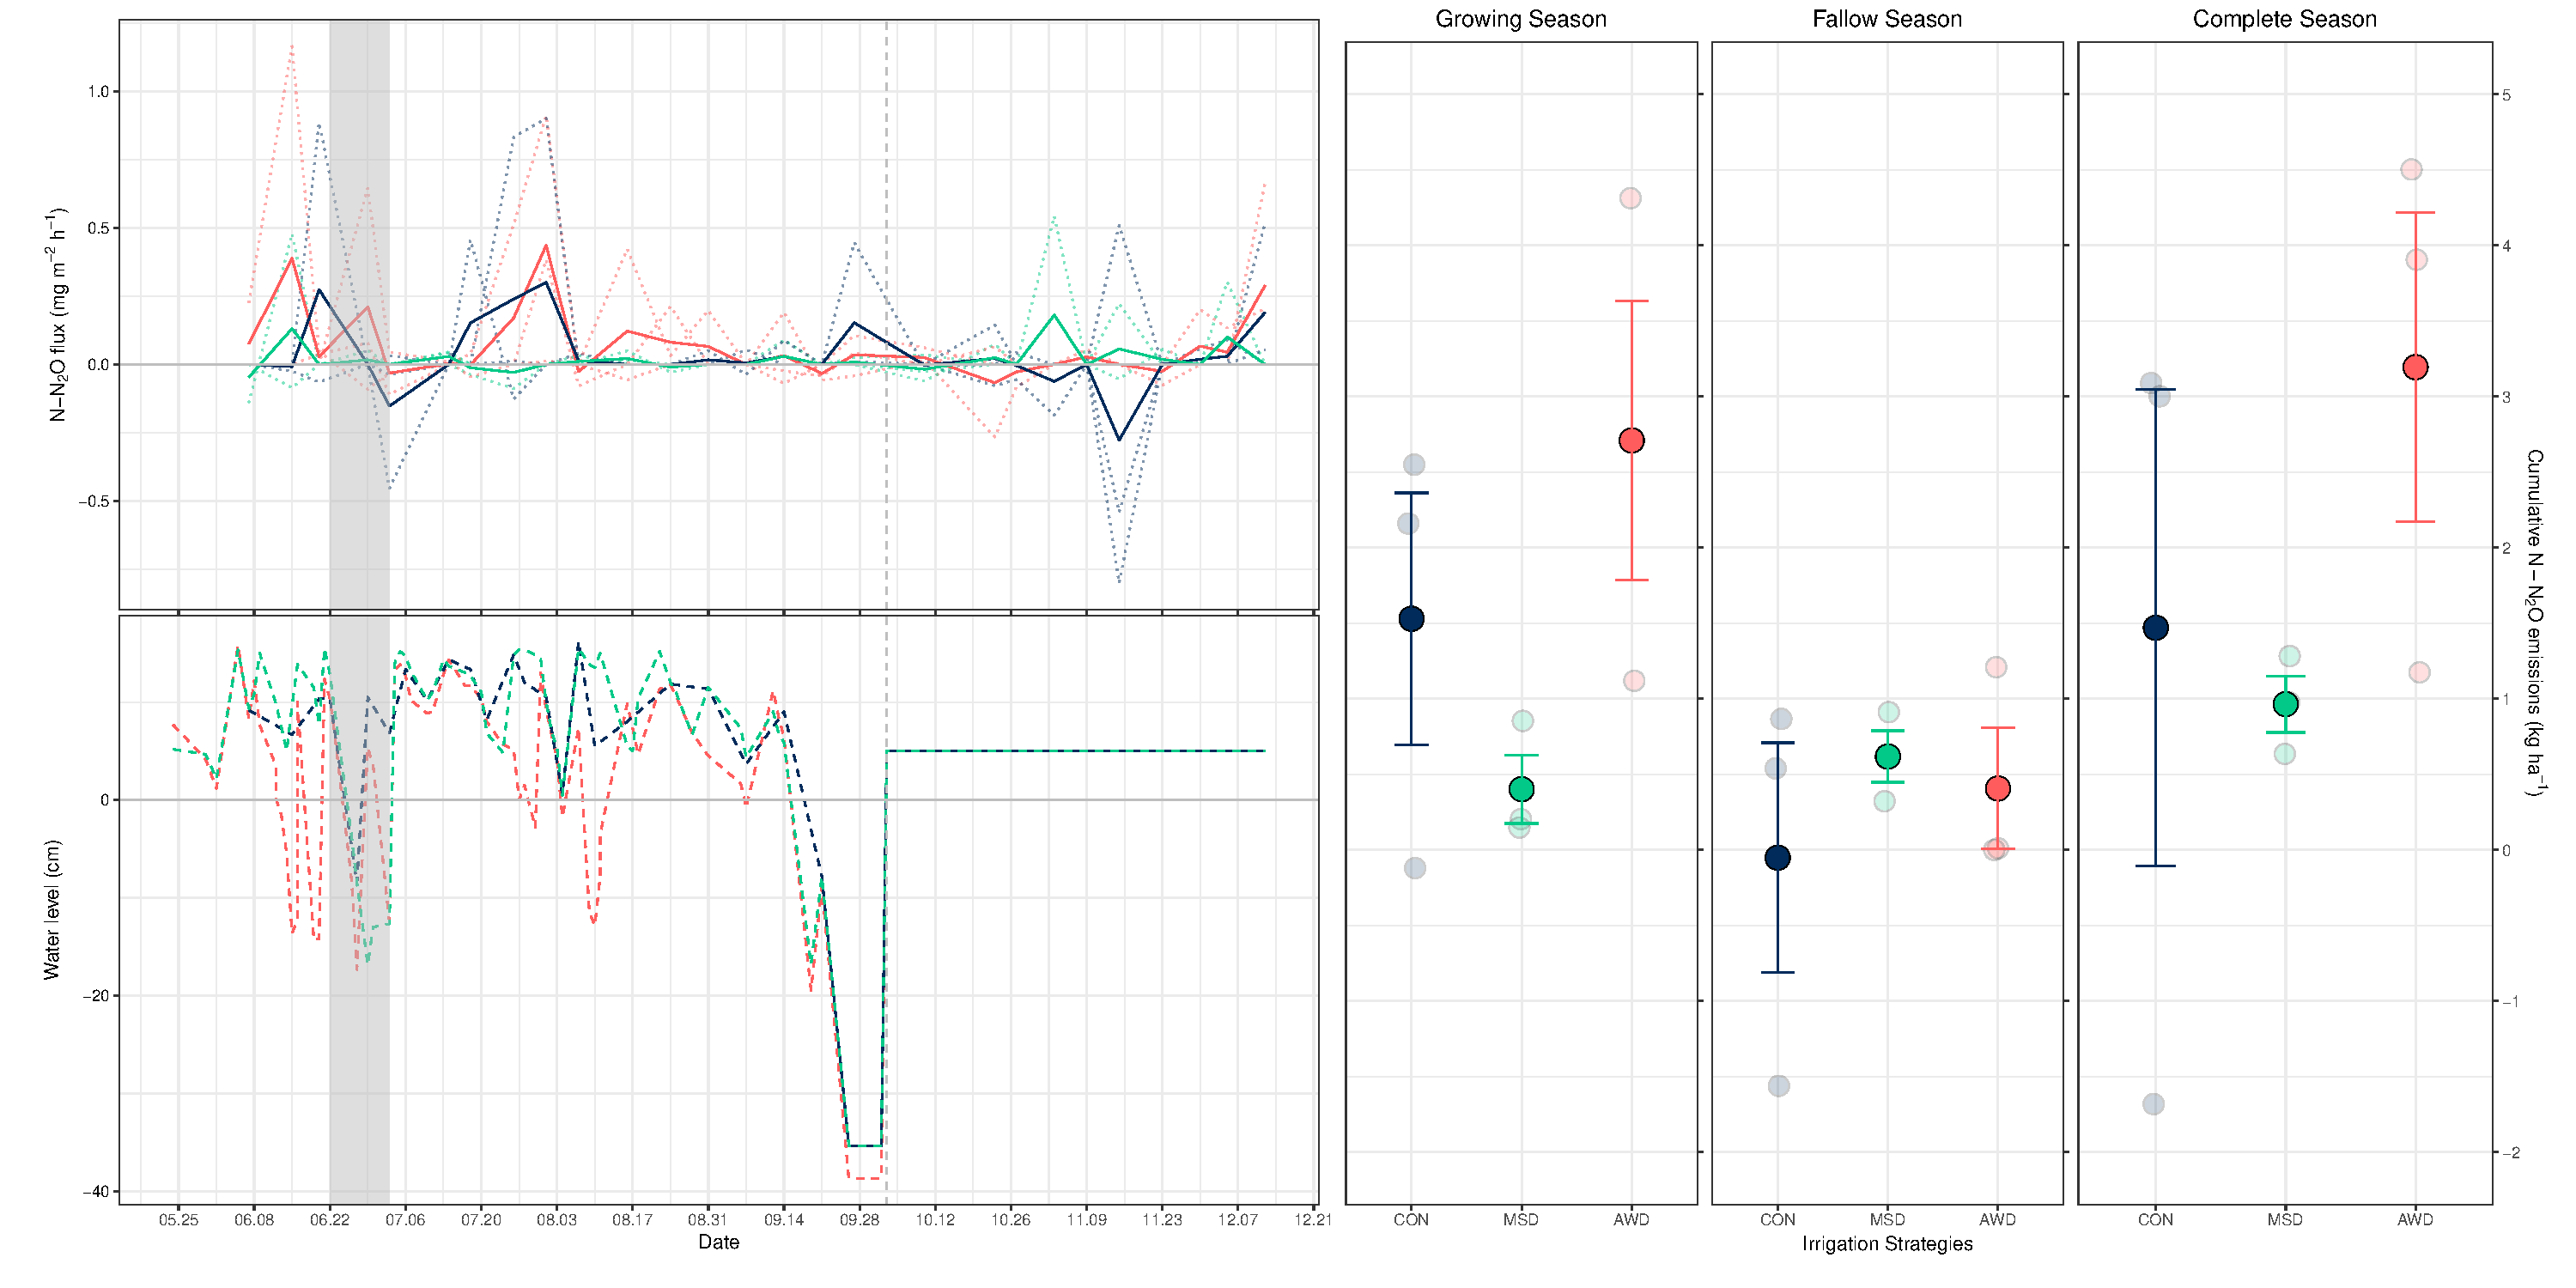
\includegraphics[scale=0.35, center]{Figures/Chapter_2/N2O_flux_acc_water.pdf}
	\captionof{figure}[Treats]{Nitrous oxide (N$_{2}$O, top-left panel) emission rates in mg m$^{-2}$ h$^{-1}$, and water level (bottom-left panel) in cm across the rice growing and fallow seasons for the three assessed irrigation strategies. Discontinuous lines in the top-left panel are mean emissions per plot, continuous lines are treatment means. Right panels show cumulative N$_{2}$O emissions in kg ha$^{-1}$ for the rice growing, fallow and complete (both growing and fallow) rice seasons. Solid dots show mean values, transparent dots show values per repetition. Error bars represent standard errors.}   
	\label{N2O}
\end{figure*}
%\vspace{0.5cm}\\

% Soil properties and Straw incorporated per mesocosm unit:

\begin{table*} [htbp]
    \centering
    \small  
    \begin{tabular}{ c | c | c }
\cline{1-3}
\multicolumn{3}{c}{Soil physicochemical properties} \\
\cline{1-3}
{Parameter} & {Value} & {Unit} \\
\cline{1-3}
{pH} & {8} & {}\\
{Electrical conductivity (25\degree C)} & {0.78} & {dS m$^{-1}$} \\
{Oxidizable organic matter} & {2.83} & {\% d.m.b$^{*}$} \\
{Equivalent Calcium Carbonate} & {36.26} & {\% d.m.b} \\
\cline{1-3}
\multicolumn{3}{c}{Soil nutrients content} \\
\cline{1-3}
{Nutrient} & {Value} & {Unit} \\
\cline{1-3}
{Nitrate} & {7.3} & {mg kg$^{-1}$ d.m.b}\\
{Phosphate} & {19.9} & {mg kg$^{-1}$ d.m.b} \\
{Potassium} & {150} & {mg kg$^{-1}$ d.m.b} \\
{Calcium} & {7,352} & {mg kg$^{-1}$ d.m.b} \\
{Magnesium} & {391} & {mg kg$^{-1}$ d.m.b} \\
{Sodium} & {251} & {mg kg$^{-1}$ d.m.b} \\
\cline{1-3}
\multicolumn{3}{c}{Straw incorporated to mesocosm units} \\
    \cline{1-3}
{Treatment} & {Mean Weight (g)} & {std. error (g)} \\ 
    \cline{1-3} 
CON & 180.00 & 17.54 \\
MSD & 175.04 & 14.69 \\
AWD & 179.22 & 5.16 \\
    \cline{1-3}
\multicolumn{3}{c}{Root biomass per irrigation strategy} \\
    \cline{1-3}
{Treatment} & {Mean Dry Weight (g)} & {std. error (g)} \\ 
    \cline{1-3} 
CON & 1.24 & 0.31 \\
MSD & 1.42 & 0.36 \\
AWD & 1.11 & 0.27 \\
\cline{1-3}
    \end{tabular}
    \caption{Soil description (physicochemical properties and nutrient content), straw incorporated to mesocosm units and root biomass per irrigation strategy. $^{*}$d.m.b = on dry matter basis}
    \label{straw}
\end{table*}

% Mesocosm setup:

\begin{figure} [ht]
\captionsetup{justification=justified}
	\centering 
	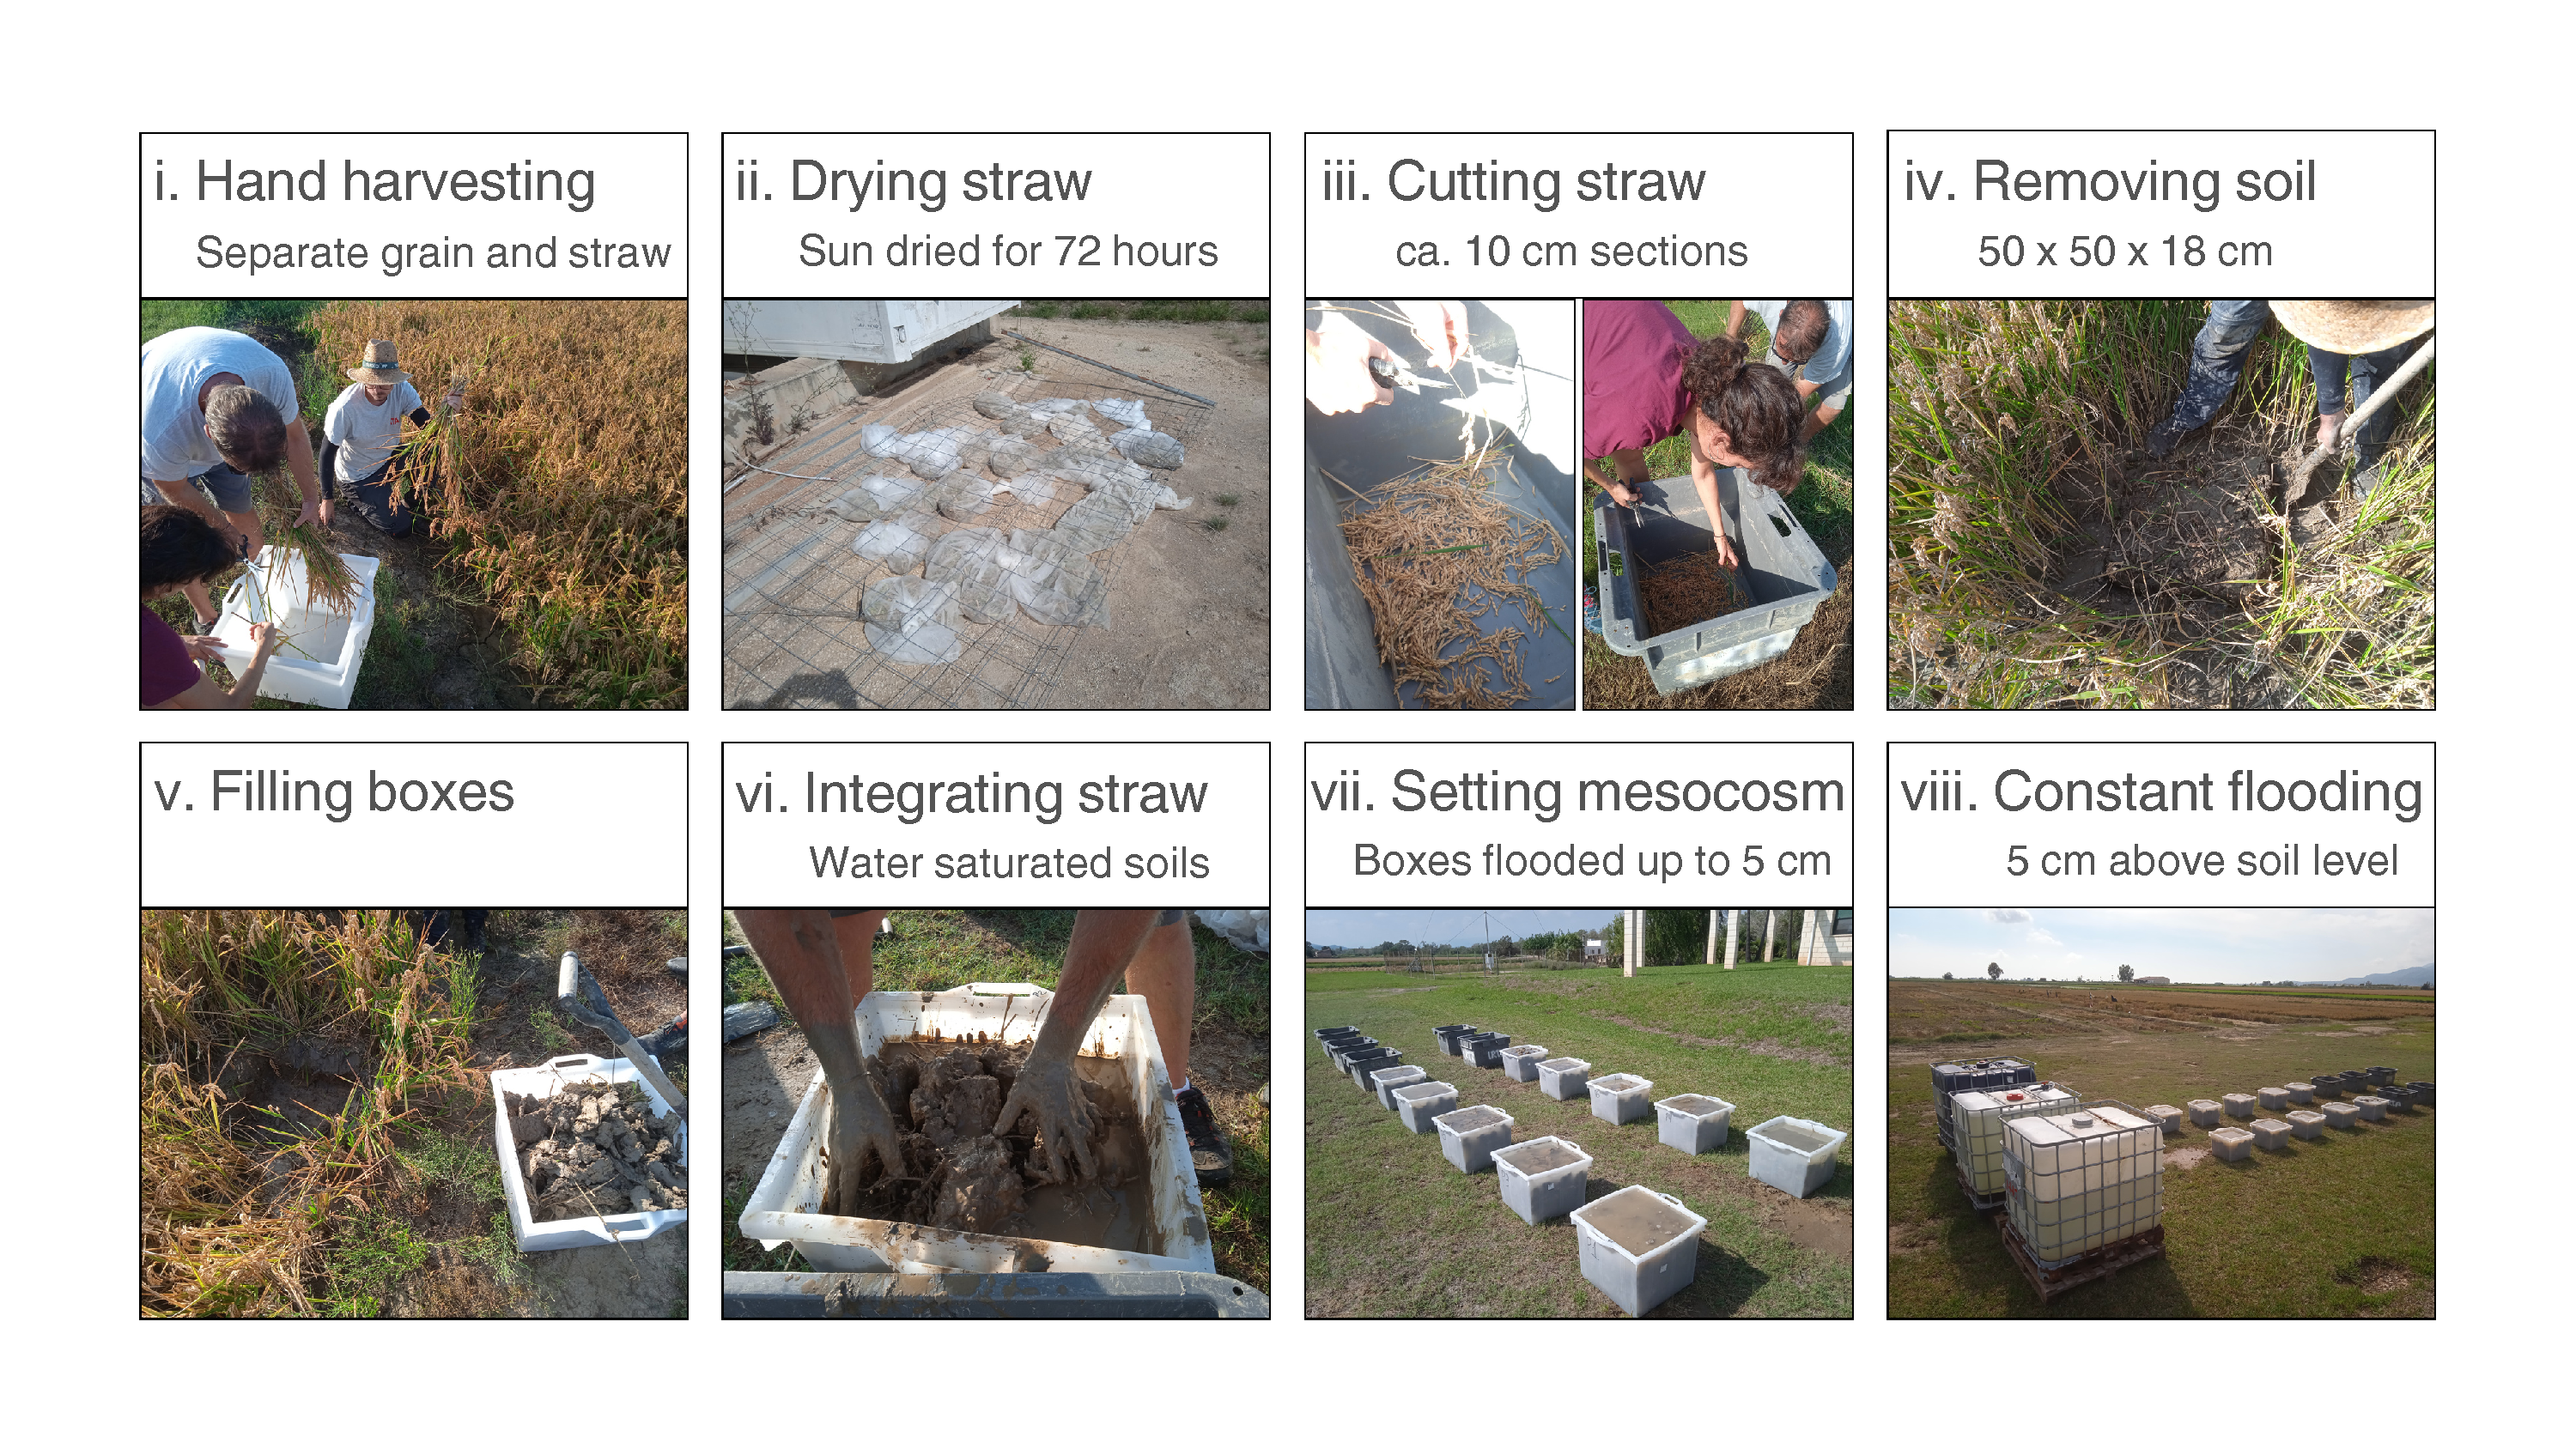
\includegraphics[scale=0.3, center]{Figures/Chapter_2/CERESTRES_meso_2023.pdf}
	\captionof{figure}[lay]{Fallow season mesocosm experiment, setup steps and layout.}  
	\label{meso}
\end{figure}
%\vspace{0.5cm}

% Weather data:

\begin{figure} [ht]
\captionsetup{justification=justified}
	\centering 
	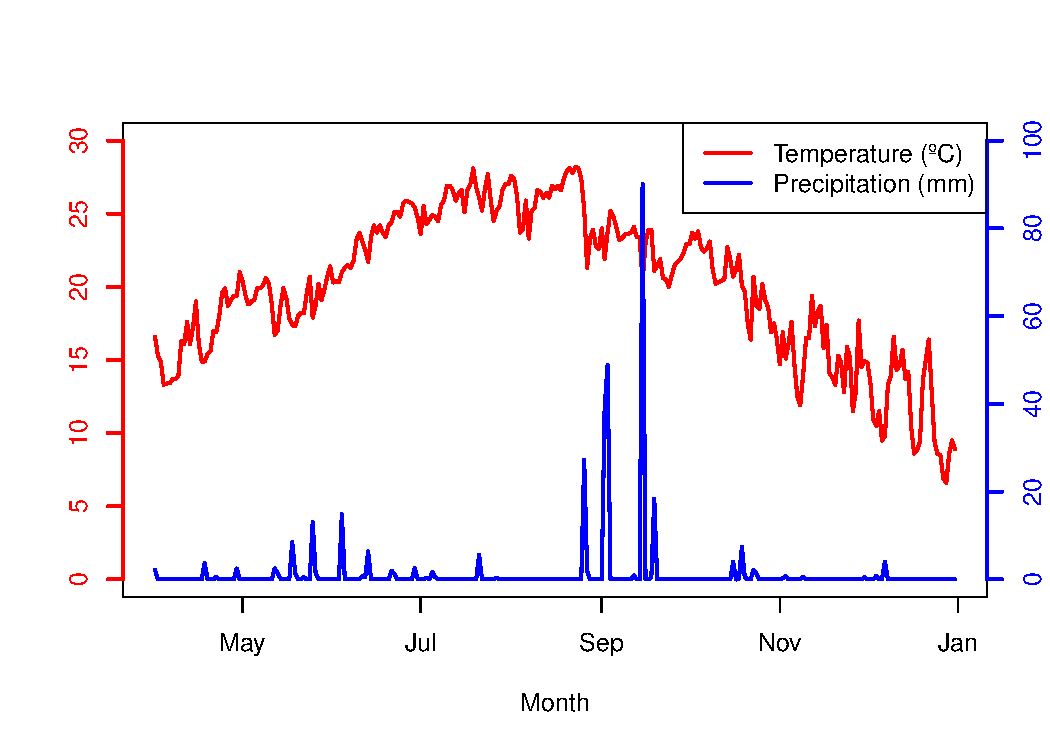
\includegraphics[scale=0.8, center]{Figures/Chapter_2/Meteocat_temp.pdf}
	\captionof{figure}[lay]{Average daily temperature (\degree C) and cumulative daily precipitation (mm) registered by an on-site meteorological station across 2023 growing and fallow seasons.}  
	\label{temp}
\end{figure}
%\vspace{0.5cm}

% Meso vs field physicochemical data:

\begin{figure} [ht]
\captionsetup{justification=justified}
	\centering 
	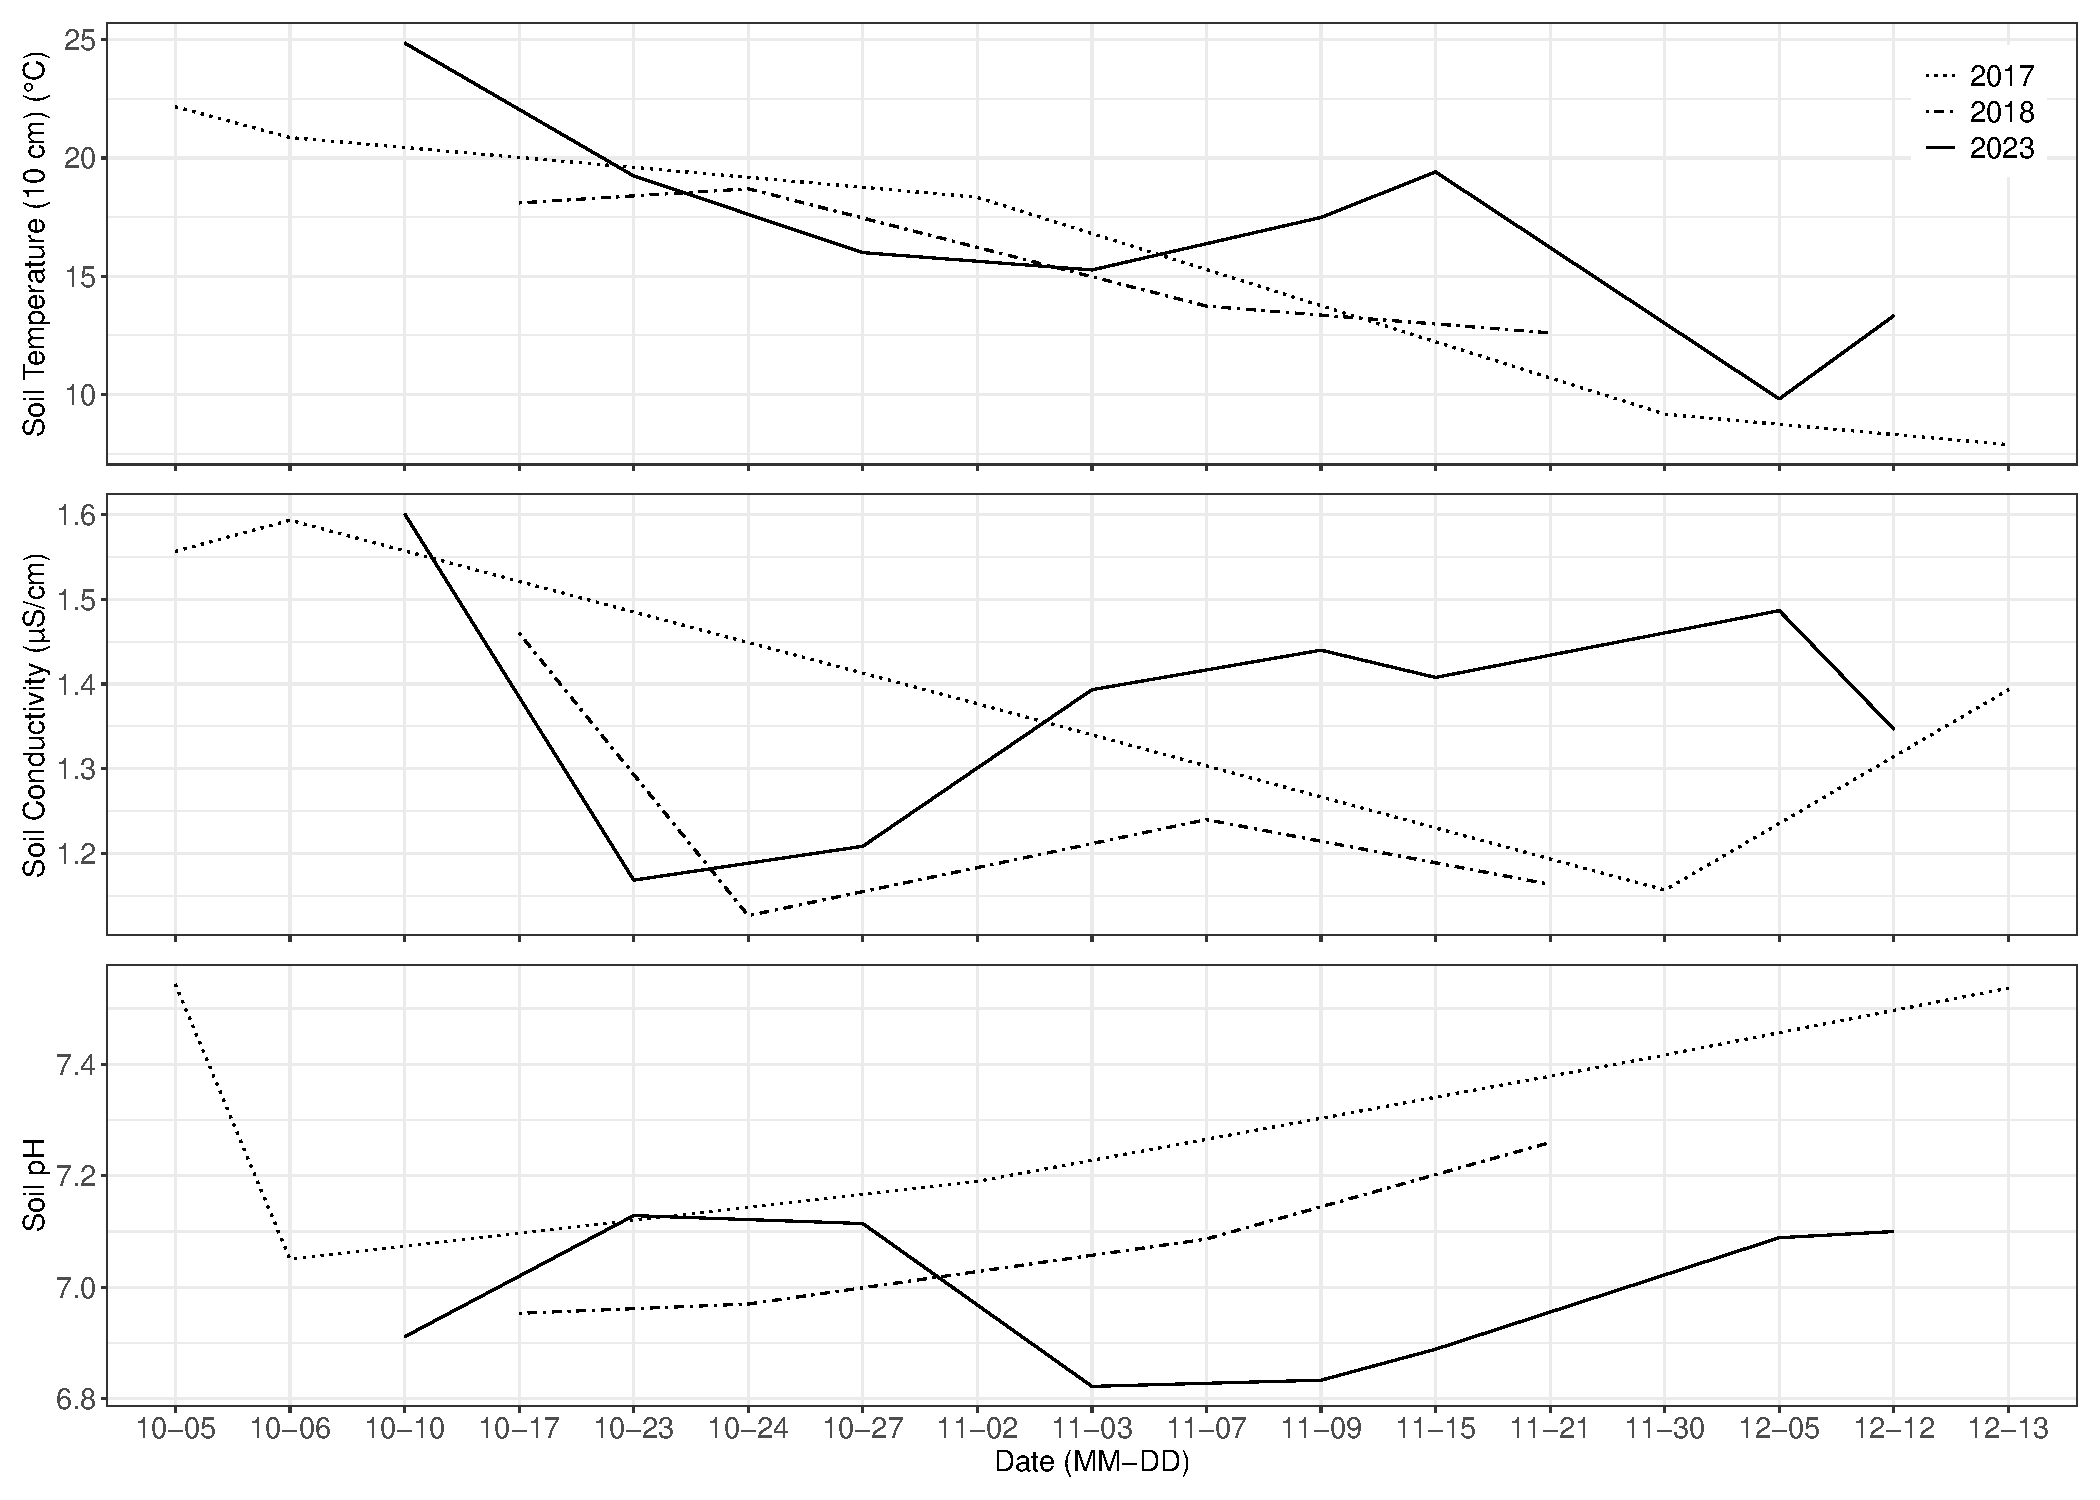
\includegraphics[scale=0.47, center]{Figures/Chapter_2/Meso_vs_Field_Plot.pdf}
	\captionof{figure}[lay]{Soil physicochemical parameters for 2017, 2018 and 2023 flooded fallow seasons. Soil temperature (\degree C) at 10 cm depth, conductivity (µS/cm) and pH. Fallow seasons 2017 and 2018 were assessed in field plots, whereas fallow season 2023 was conducted in mesocosm units. All measurements were done in plots within the IRTA Ebro Experimental Station facilities in Amposta, securing constant soil texture.}  
	\label{meso_field}
\end{figure}
%\vspace{0.5cm}

%\end{document}

% Restore normal figure and table numbering
\renewcommand{\thefigure}{\thechapter.\arabic{figure}}
\setcounter{figure}{0}

\renewcommand{\thetable}{\thechapter.\arabic{table}}
\setcounter{table}{0}
 
%\include{Chapters/Chapter3}
%\include{Chapters/Chapter4} 
%\include{Chapters/Chapter5} 

%----------------------------------------------------------------------------------------
%	THESIS CONTENT - APPENDICES
%----------------------------------------------------------------------------------------

%\appendix % Cue to tell LaTeX that the following "chapters" are Appendices - Seba: commented out

% Include the appendices of the thesis as separate files from the Appendices folder
% Uncomment the lines as you write the Appendices

%\include{Appendices/AppendixA} - Seba: commented out
%\include{Appendices/AppendixB}
%\include{Appendices/AppendixC}

%----------------------------------------------------------------------------------------
%	BIBLIOGRAPHY
%----------------------------------------------------------------------------------------

%\printbibliography[heading=bibintoc] Seba: made note

\bibliography{PhD_Thesis_bib}

%----------------------------------------------------------------------------------------

\end{document}  